\documentclass[defaultstyle,11pt]{thesis}

%%%%%%%%%%%%%%%%%%%%%%%%%%%%%%%%%%%%%%%%%%%%%%%%%%%%%%%%%%%%%%%%
%%%%%%%%%%%  see documentation for information about  %%%%%%%%%%
%%%%%%%%%%%  the options (11pt, defaultstyle, etc.)   %%%%%%%%%%
%%%%%%%  http://www.colorado.edu/its/docs/latex/thesis/  %%%%%%%
%%%%%%%%%%%%%%%%%%%%%%%%%%%%%%%%%%%%%%%%%%%%%%%%%%%%%%%%%%%%%%%%
%		\documentclass[typewriterstyle]{thesis}
% 		\documentclass[modernstyle]{thesis}
% 		\documentclass[modernstyle,11pt]{thesis}
%	 	\documentclass[modernstyle,12pt]{thesis}

%%%%%%%%%%%%%%%%%%%%%%%%%%%%%%%%%%%%%%%%%%%%%%%%%%%%%%%%%%%%%%%%
%%%%%%%%%%%    load any packages which are needed    %%%%%%%%%%%
%%%%%%%%%%%%%%%%%%%%%%%%%%%%%%%%%%%%%%%%%%%%%%%%%%%%%%%%%%%%%%%%
\usepackage{graphicx}		% to insert PostScript figures
\usepackage{rotating}		% for sideways tables/figures
\usepackage{subfigure}
\usepackage{fancyvrb}
\usepackage{multicol}
\usepackage{booktabs}
%\usepackage{hyperref}
\usepackage{amsmath, amsthm, amssymb}
\usepackage{latexsym}		% to get LASY symbols
\usepackage{rotating}		% for sideways tables/figures
\usepackage{multirow}		% support multiple/single rows simultaneously in table
\usepackage{float}
\usepackage{wrapfig}
\usepackage{subfigure}
\usepackage{fancyvrb}
\usepackage[usenames,dvipsnames]{color}
\usepackage{microtype}
\usepackage{times}
\usepackage{amssymb}
\usepackage{epstopdf}
\usepackage{moreverb}
\usepackage{url}
\usepackage{verbatim}
\usepackage{cite}
\usepackage{listings}
\usepackage{footmisc}
\usepackage{algorithm}
\usepackage{algorithmic}
\usepackage{hevea}
\usepackage{array}
\usepackage{layouts}
\usepackage{longtable}
\usepackage{threeparttable}

\newtheorem{con}{Conjecture}
\newtheorem{thm}{Theorem}
\newtheorem{lem}[thm]{Lemma}
\newtheorem{corollary}[thm]{Corollary}

\newcommand{\ra}[1]{\renewcommand{\arraystretch}{#1}}

\newcommand{\La}{\langle}
\newcommand{\Ra}{\rangle}
\newcommand{\Comment}[2]{{\color{red}\emph{[#2 --#1]}}}
\newcommand{\M}{\mathit}
\newcommand{\C}{\prec \succ}

\DefineShortVerb{\@}

\DefineVerbatimEnvironment%
  {Verb}{Verbatim}
  {framesep=2mm, rulecolor=\color{ForestGreen}}

\DefineVerbatimEnvironment%
  {VerbWithNumbers}{Verbatim}
  {fontsize=\small, framesep=2mm, rulecolor=\color{ForestGreen}, 
   numbers=left, numbersep=3pt, stepnumber=1}


%%%%%%%%%%%%%%%%%%%%%%%%%%%%%%%%%%%%%%%%%%%%%%%%%%%%%%%%%%%%%%%%
%%%%%%%%%%%%       all the preamble material:       %%%%%%%%%%%%
%%%%%%%%%%%%%%%%%%%%%%%%%%%%%%%%%%%%%%%%%%%%%%%%%%%%%%%%%%%%%%%%
\title{Dynamic Trace Analysis with Zero-Suppressed BDDs}

\author{Graham David}{Price}

\otherdegrees{B.S. University of Evansville, 2002\\
  M.S. University of Colorado at Boulder, 2006}

\degree{Doctor of Philosophy}		%  #1 {long descr.}
	{Ph.D., Electrical, Computer, and Energy Engineering}		%  #2 {short descr.}

\dept{Department of}			%  #1 {designation}
	{Electrical, Computer, and Energy Engineering}		%  #2 {name}

\advisor{Professor}				%  #1 {title}
	{Manish Vachharajani, Ph.D. (Chair)}			%  #2 {name}

\reader{Fabio Somenzi, Ph.D.}			%  #2 {name}
\readerThree{Bor-Yuh Evan Chang, Ph.D.}		%  2nd person to sign thesis
\readerFour{Jeremy G. Siek, Ph.D.}		%  3rd person to sign thesis
\readerFive{Tipp Moseley, Ph.D. (Outside Member)}	%  4rd person to sign thesis

\abstract{ \OnePageChapter % one page only ??  

Instruction level parallelism (ILP) limitations have forced processor
manufacturers to develop multi-core platforms with the expectation
that programs will be able to exploit thread level parallelism
(TLP). Multi-core programming shifts the burden of locating additional
performance away from computer hardware to the software developers,
who often attempt high-level redesigns focused on exposing thread
level parallelism, as well as explore aggressive optimizations for
sequential codes.

Precise dynamic analysis can provide useful guidance for program
optimization efforts, including efforts to find and extract
thread level parallelism.  Unfortunately, finding regions of code
amenable to further optimization efforts requires analyzing traces
that can quickly grow in size.  Analysis of large dynamic traces
(e.g. one billion instructions or more) is often impractical for
commodity hardware.

An ideal representation for dynamic trace data would provide
compression.  However, decompressing large software traces, even if
decompressed data is never permanently stored, would make many
analysis impractical.  A better solution would allow analysis of the
compressed data, without a costly decompression step. Prior works have
developed trace compressors that generate an analyzable
representation, but often limit the precision or scope of analyses.

Zero-suppressed binary decision diagram (ZDDs) exhibit many of the
desired properties of an ideal trace representation.  This thesis
shows: (1) dynamic trace data may be represented by zero-suppressed
binary decision diagrams (ZDDs); (2) ZDDs allow many analyses to
scale; (3) encoding traces as ZDDs can be performed in a reasonable
amount of time; and, (4) ZDD-based analyses, such as irrelevant
instruction detection and potential coarse-grained thread level
parallelism extraction, can reveal a number of performance
opportunities in sequential programs.
}

\dedication[Dedication]{	% NEVER use \OnePageChapter here.
%  To Lea
}

\acknowledgements{\OnePageChapter	% *MUST* BE ONLY ONE PAGE!

%  I would like to acknowledge that this thesis only exists in cyberspace.

}

\ToCisShort	% a 1-page Table of Contents ??

\LoFisShort	% a 1-page List of Figures ??
%	\emptyLoF	% no List of Figures at all ??

%\LoTisShort	% a 1-page List of Tables ??
\emptyLoT	% no List of Tables at all ??


%%%%%%%%%%%%%%%%%%%%%%%%%%%%%%%%%%%%%%%%%%%%%%%%%%%%%%%%%%%%%%%%%
%%%%%%%%%%%%%%%       BEGIN DOCUMENT...         %%%%%%%%%%%%%%%%%
%%%%%%%%%%%%%%%%%%%%%%%%%%%%%%%%%%%%%%%%%%%%%%%%%%%%%%%%%%%%%%%%%

%%%%  footnote style; default=\arabic  (numbered 1,2,3...)
%%%%  others:  \roman, \Roman, \alph, \Alph, \fnsymbol
%	"\fnsymbol" uses asterisk, dagger, double-dagger, etc.
%	\renewcommand{\thefootnote}{\fnsymbol{footnote}}
%	\setcounter{footnote}{0}

\begin{document}

%%%%%%%%%%%%%%%%%%%%%%%%%%%%%%%%%%%%%%%%%%%%%%%%%%%%%%%%%%%%%%%%%%%%%%%%%%%%%
\chapter{Introduction}
%%%%%%%%%%%%%%%%%%%%%%%%%%%%%%%%%%%%%%%%%%%%%%%%%%%%%%%%%%%%%%%%%%%%%%%%%%%%%

Instruction level parallelism (ILP) limitations have forced processor
manufacturers to develop multi-core platforms with the expectation
that programs will be able to exploit thread level parallelism
(TLP)~\cite{ali-reza:2007:ppopp, intel:2005:dual, intel:2005:dual2}.
This shift forces software engineers to try and improve the
performance of their applications with high-level redesigns focused on
exposing parallelism, as well as explore aggressive optimizations for
sequential codes~\cite{park:2001lr, herlihy:2006:oopsla}. Extracting
TLP by manual high-level software redesign is often
difficult~\cite{herlihy:2008:art}. Instruction level dynamic program
analysis can provide useful guidance for program optimization,
including efforts to find and extract thread level parallelism.
However, optimizations often exist within large dynamic
traces~\cite{iyer:05:epic}, and finding opportunities for performance
can require the analysis of gigabytes of trace data.  This thesis
shows that: (1) Zero-Suppressed Binary Decision Diagrams (ZDDs)
enables many analyses to scale; (2) ZDD creation is practical for
traces of a billion instructions for a variety of benchmarks; and, (3)
ZDD-based analysis, such as irrelevant instruction detection and
potential coarse-grained thread level parallelism extraction, can
reveal a number of performance opportunities that exist in sequential
programs.

\section{Dynamic Trace Compression}

Dynamic trace analysis has been used in prior work for performance
tuning and hardware debugging~\cite{wu:94:micro}. Unfortunately, trace
files can easily grow to terabytes in size depending on the
information collected and the duration of traced execution.  Large
dynamic trace sizes (e.g. 1 billion instructions or more) can make
analysis and visualization impractical.

Researchers have developed streaming compression algorithms (e.g.,
Burtscher \textit{et. al.}~\cite{burtscher:05:cgo}) that can compress
these traces by a factor of 10 or more.  Unfortunately, these
techniques do not speed trace analysis.  Compression techniques force
analyzers to stream a decompressed version of the trace through the
analysis engine.  Thus, analyses have complexity that depends on the
\textit{decompressed} trace size, even though the decompressed trace
is never stored on disk.  With large traces, this time-consuming
process prohibits certain global analyses and interactive tools.
Examples of prohibitively expensive operations include memory-data
liveness visualization, hot code visualization, trace
slicing~\cite{zhang:04:icse}, and interactive visualization of thread
level parallelism.

Ideally, a compressed trace format should allow analyses to operate
directly on the compressed representation with complexity that is a
function of \textit{compressed} trace size.  Then, if large portions
of compressed traces fit in memory, global analyses and interactive
visualization become possible.  Larus \textit{et. al.} propose such a
technique for \textit{whole program path}
analysis~\cite{larus:99:pldi}.  The technique uses the SEQUITUR
compression method and works well for finding sequence matches in
program execution.  However, \textit{whole program path} analysis does
not permit direct application of data-centric analyses (e.g., trace
slicing) that are of interest to system designers and programmers.
Recent work on stride compression techniques addresses this issue by
forming hierarchies based on accessed memory
regions~\cite{minjang:10:micro}, but is limited to analyses based on
loop-level dependence.

This thesis explores reduced, ordered, binary decision diagram
(ROBDDs)~\cite{bryant:86:ieeetc}, originally developed for hardware
verification, as a trace representation for dynamic program analysis.
BDDs can provide compression for large sets of data whose size would
otherwise make analysis intractable.  For example, BDDs in hardware
verification and validation allow equivalence checking of circuits
with many states in constant time~\cite{brayton:96:cav}.  In program
analysis, BDDs have been used to store program contexts for each
object in a program analysis lattice object~\cite{whaley:07:thesis}.
When BDDs are used for the analysis of large program
traces~\cite{price:06:cal,price:08:pact,zhang:04:icse}, the size of
dynamic program traces can be reduced by up to 60x when encoded as a
BDD~\cite{price:06:cal}.  Further, this compressed representation can
be analyzed without decompression, with algorithmic complexity that is
a function of the compressed size~\cite{price:06:cal}.  Thus,
trace-encoded BDDs provide a solution to the dynamic trace size issue
by representing trace information in a compressed, yet analyzable,
structure.

\section{Dynamic Trace Analysis at Scale}

Encoding large traces as BDDs can be time consuming, requiring hours
to days to complete~\cite{price:08:msthesis}.  This in turn makes
tools that use BDD-based representations less effective than otherwise
possible.  Prior applications of BDDs depend on three methods to
mitigate BDD creation time: (1) search for a variable order that
allows for fast BDD creation, (2) tune the tables and caching systems
used in many BDD packages, and (3) encode an abstraction of the
original data set.  This thesis discusses zero-suppressed BDDs (ZDDs)
as an alternative to BDDs in order to reduce creation time for large
traces.  Prior work has shown that ZDDs can reduce the final BDD size
for sparse data and context data used during static program
analysis~\cite{minato:01:STTT, lhotak:08:lcpc}, though this work has
not applied ZDDs to compressing dynamic trace data.  This thesis shows
that, without data loss, ZDD-based SPEC INT 2000 benchmark traces are
25\% smaller than BDD-based traces.

Traces from a variety of applications need be analyzed to demonstrate
the efficacy of ZDD-based dynamic trace analysis.  Reducing trace
creation time by 25\%, which intuitively should correspond to the 25\%
reduction in representation size, is beneficial, but simply not enough
to allow analysis of billions of instructions from a variety of
benchmarks.  Initial tests of ZDD creation time proved to be far
worse; the 25\% reduction in representation size did not translate to
25\% reduction in creation time.  ZDDs creation time was, for some
benchmarks, $3\times$ slower.  Further investigation revealed a
modification to the caching mechanism will remove this penalty in most
cases.  In fact, ZDD-based trace compression algorithms have a smaller
working set size making tuning possible for large traces, which
results in a creation time that can be $9\times$ faster than BDD
creation time for the same benchmark.  A detailed discussion of
ZDD-based trace compression can be found in Chapter~\ref{chap:scale}.

\section{Opportunities for Optimization}

Reducing ZDD creation time is crucial to explore opportunities for
optimization in a wide range of program
traces. Chapter~\ref{chap:tlpstudy} explores potential coarse-grained
thread level parallelism (TLP) that exists in sequential applications.
Chapter~\ref{chap:deadcode} demonstrates the use of ZDD-encoded traces
to locate irrelevant instruction chains.

\noindent\paragraph{Irrelevant Instruction Elimination}

Irrelevant component elimination has been used in prior work to
simplify abstractions for static analysis~\cite{corbett:icsc:2000}.
This thesis uses an irrelevant component elimination with ZDD-encoded
precise dynamic instruction dependencies.  This thesis will show that
ZDD-based irrelevant instruction dependency elimination can locate
instructions that fail to the following criteria: (1) the instruction
dependence chain should reach the end of the program trace; or, (2)
the dependence chain should produce an output through a Linux system
call.

ZDD-based irrelevant instruction dependency elimination is designed to
iterate irrelevant code calculation until convergence.  However,
irrelevant instruction dependency elimination can take days to
complete for traces with long dynamic dependency chains. Empirical
data presented in this thesis shows that, for all benchmarks in SPEC
2006 INT, the irrelevant instruction elimination algorithm reaches a
steady state.  In this state, the number of instruction dependencies
removed per slice iteration oscillates, but will not monotonically
decrease until the analysis converges.  Thus, it is possible to
approximate the number of instructions removed by iterating irrelevant
instruction elimination until oscillation is detected.

ZDD-based irrelevant instruction dependency elimination may also be
used to filter irrelevant points from program visualizations. However,
irrelevant instruction dependency elimination may also be used as a
technique for code optimization or compiler evaluation.
Chapter~\ref{chap:deadcode} contains a survey of irrelevant code
removal from the SPEC 2006 INT benchmarks using both \textit{-O0} and
\textit{-O2} optimization levels in the \textit{gcc} compiler.

\noindent\paragraph{Hot-Code Visualization}

In addition to the optimization analyzes presented in this thesis,
which include coarse-grained thread level parallel region location and
irrelevant instruction elimination, a hot-code visualization algorithm
was created to focus optimization efforts on the most frequently
executed regions of code.

Hot-code analysis captures static instruction execution frequency and
counts the frequency of execution.  The static hot code information is
combined with a mapping from $dynamic\ instruction \ \rightarrow
\ static\ instructions$ to create a new relation from each dynamic
instruction to hot-code value.  The resulting visualizations can be
found in Appendix~\ref{appdx:hotcode2000} and
Appendix~\ref{appdx:hotcode2006}.

\section{Contributions}

Traces from a variety of applications need be analyzed to demonstrate
the efficacy of DD-based dynamic trace analysis. The results in this
thesis show that ZDD-based trace compression results in 25\% smaller
representation compared to BDD-based traces.  Further, ZDDs have a
smaller working set, thus the ZDD creation package can tuned to cache
the working set of the trace-ZDD during creation.  This reduces the
number of garbage collection operations and removal of useful dead
nodes. This reduces DD creation by up to 9$\times$.

Hot code analysis can tell developers where to focus optimization and
parallelization efforts. In addition to the optimization analyzes
presented in this thesis, which include coarse-grained thread level
parallel region location and irrelevant instruction elimination, a
hot-code visualization algorithm was created to focus optimization
efforts on the most frequently executed regions of code.

The results from a survey of irrelevant instructions in the SPEC 2006
INT benchmark shows that over 50\% of instruction dependencies do not
produce a value and do not reach the end of the program trace.  It is
possible for an instruction to be relevant to program execution but
not meet the specified requirements.  Therefore, this thesis also
presents results comparing the irrelevant dependence counts from both
the \textit{-O0} and \textit{-O2} compiler settings. The irrelevant
dependency count from the \textit{-O0}, or non-optimized, compiler
setting provides a worst-case value to normalize further comparison
operations.  Furthermore, this technique can test the effectiveness of
static compiler optimizations, as well as locate potential irrelevant
instruction streams.

This thesis explores potential coarse grain TLP that may be
exploitable in conjunction with TLS and ILP techniques.  In
particular, the thesis examines the SPEC INT 2006 benchmark suite,
looking for parallelism with a granularity of thousands of dynamic
instructions, and is not restricted to loop-level TLP. The survey
presented in Chapter~\ref{chap:tlpstudy} found, on average, 7\% of
instructions may be extracted as course-grained parallelism, and for
the benchmark 445.gobmk, 44\% of instructions may be extracted as
coarse-grained TLP.

\noindent\paragraph{Potential Coarse-Grained Thread Level Parallelism}

An effective, popular, and widely studied mechanism for automatically
exploiting parallelism is to dynamically and speculatively thread
groups of
instructions~\cite{steffan:00:isca,prabhu:03:ppopp,wu:2008:cdp,chen:cc:2004,vachharajani:07:pact,dou:2007:trans,wang:2009:dps,marcuello:00:ipdps,bridges:2007:micro,thies:2007:micro,raman:2010:asplos}.
Recent advances in this thread level speculation~(TLS) can parallelize
execute over 90\% of some codes~\cite{marcuello:00:ipdps}.  However,
TLS predictor accuracy limits TLS to fine-grained or loop-level
TLP~\cite{marcuello:00:ipdps,warg:2001:pact,bridges:2007:micro,thies:2007:micro,raman:2010:asplos}.

This thesis explores potential coarse grain TLP that may be
exploitable in conjunction with TLS and ILP techniques.  In
particular, the thesis examines the SPEC INT 2006 benchmark suite,
looking for parallelism with a granularity of thousands of dynamic
instructions, and is not restricted to loop-level TLP.  Coarse-grained
TLP is located using the ParaMeter dynamic trace visualization
tool~\cite{price:08:pact}.  This technique, which is discussed in
Section~\ref{sec:parameter}, generates a visualization of program
execution, called a DINxRDY (dynamic instruction number by ready time)
plot.  This plot visually shows potential coarse grain TLP as lines
that overlap on the x-axis.

Potential parallel regions found within DINxRDY plots are further
analyzed to expose dependence relationships.  Inter-region dependence
conflicts, discussed in Section~\ref{sec:chop} are found by dynamic
dependence graph (DDG)
slicing~\cite{gallager:91:se,agrawal:90:pldi,agrawal:92:thesis,korel:88:ipl}.
Slicing DDGs that contain a large number of instructions
(e.g. billions) can take weeks~\cite{agrawal:90:pldi, zhang:03:icse}.
To efficiently, and precisely, explore the dependency relationships
between two regions of code this thesis extends the DDG \textit{chop}
to use the ZDD-compressed trace format.  The dynamic
chop~\cite{gupta:2005:ase, krinke:2004:sqc} is often faster than an
intersection of a forward and reverse slice and requires no loss of
precision.

The survey presented in Chapter~\ref{chap:tlpstudy} found, on average,
7\% of instructions may be extracted as course-grained parallelism,
and for the benchmark 445.gobmk, 44\% of instructions may be extracted
as coarse-grained TLP.

Finally, a summary of contributions, techniques, and results of this
thesis may be found in Chapter~\ref{chap:conclusion}.

Thus, this thesis presents the following contributions:

\begin{enumerate}
\item A ZDD-based trace compression algorithm with tuning for large
  traces, resulting in a 25\% reduction in BDD size and a $9\times$
  reduction in trace compression time.
\item A ZDD-based iterative analysis for locating irrelevant
  instruction dependencies
\item A method to quickly explore coarse-grained parallelism in serial
  applications.
\item A ZDD-based dependence graph chopping algorithm need for the
  aforementioned method.
\item A survey of coarse-grained thread level parallelism in the SPEC
  INT 2006 benchmarks that shows up to 44\% of instructions may be
  extractable as coarse grain TLP.
\end{enumerate}

\section{Hypothesis}

\emph{ZDD-based dynamic trace analysis can identify hot-code paths,
  irrelevant instructions, and potential coarse-grained thread level
  parallelism in sequential codes, and thus create opportunities for
  program optimization.}


%%%%%%%%%%%%%%%%%%%%%%%%%%%%%%%%%%%%%%%%%%%%%%%%%%%%%%%%%%%%%%%%%%%%%%%%%%%%%
\chapter{Parallel Computation Background}
\label{chap:parallelBackground}
%%%%%%%%%%%%%%%%%%%%%%%%%%%%%%%%%%%%%%%%%%%%%%%%%%%%%%%%%%%%%%%%%%%%%%%%%%%%%

Parallel computation is a source for performance for both software and
hardware in many modern computer
systems~\cite{ali-reza:2007:ppopp,intel:2005:dual, intel:2005:dual2}.
Correct manual thread level parallelization of software can be
difficult, may result in non-deterministic errors, and often the
resulting parallel application is often harder to debug than a
sequential
application~\cite{herlihy:2008:art,lamport:1978:tco,fridge:88:padd}. This
thesis explores software tools that help a developer find and extract
parallelism. Parallel computation and parallel programming would
require volumes to discuss
completely~\cite{lea:1996:cpij,herlihy:2008:art}.  This thesis
requires an understanding of three attributes of parallel tasks: (1)
location; (2) granularity; and, (3) conflicts.   Prior works have
researched both automatic and manual techniques for defining the
location, granularity, and conflicts in potential parallel tasks.
Following a discussion on these topics, this chapter will then explore
static and dynamic techniques that can locate parallel tasks and task
conflicts.

\section{Automatic Parallelization Techniques}

Automatic parallelization is a heavily research
field~\cite{hoeflinger:98:uiuccs, blume:1992:pds, Hall:2005wd}.
Parallel task location and granularity are defined by instructions
contained within a parallel task boundary~\cite{chen:1990:isca}.
Conflicts between parallel tasks often occur from read-after-write
hazards; if a task alters a value read by a different parallel task
can result in unexpected program execution.  This section looks at
static and dynamic techniques for automatically finding parallel task
locations, boundries, and conflicts.

\subsection{Automatic Parallelization by Static Analysis}

The location of parallelism can be determined a statically before
program execution by a
compiler~\cite{bringmann:95:uiuccs,dou:2007:trans}.  The example code
in Figure~\ref{fig:parallelpseudosrc} can help explain how to find
parallel tasks and task boundaries using only static program
information.  An illustration of the sequential execution of the
source in Figure~\ref{fig:parallelpseudosrc} can be seen in
Figure~\ref{fig:parallelpseudoseq}.  This code is in C/C++ style, and
contains many pointer operations to demonstrate the limitations of some
analysis methods.  In line 1, the variable \textit{a} is a integer
pointer variable, and the arrayB contains integers.  Thus, line 1 sets
the value of \textit{a} to a pointer to the fourth member of arrayB.

\begin{figure}
  \begin{lstlisting}
    
1:    a = &(arrayB[4])

2:    for (i = 0; i < arrayB.size(); ++i)
3:    {
4:      b = funcA()
5:      c = arrayB[i]
6:      arrayB[b + c] = i
7:    }
    
8:    print(*a)
9:    print(b)

  \end{lstlisting}
  \caption{Parallel Pseudo Code Example}
  \label{fig:parallelpseudosrc}
\end{figure}

The next point of heap obfuscation occurs inside the control flow test
in line 2. The function \textit{size} is a member of the array type
used in this pseudo code.  This function the determines the size of
the array, which can be difficult to determine at run-time.  Thus, a
static analysis would likely need to be \textit{context sensitive} and
\textit{interprocedural}.  Context sensitivity allows the analysis to
understand the difference, or similarities, between multiple
occurrences of the same static code~\cite{emami:94:pldi}.  An
interprocedural analysis allows the analysis to go into, and out from,
a function call during analysis~\cite{allen:76:cacm}.  A context
sensitive and interprocedural analysis would still need to determine
the size of the array \textit{arrayB} which was likely allocated using
heap memory.  In languages that allow heap allocation and references,
the size and value of heap memory is difficult to determine at
compile-time difficult~\cite{kong:91:test, muchnick:97:mkp,
  towle:76:uiuccs}.  

The size of the array may require an expensive points-to
analysis~\cite{steensgaard:96:popl}, or, if the size of the array
varies with a run-time input, than the size of the array could not be
found by static analysis. Interprocedural static analysis, such as
\textit{points-to}~\cite{steensgaard:96:popl} and
\textit{alias}~\cite{cooper:89:popl} can find conflicts between
instructions.

The final heap accesses in the pseudo code in
Figure~\ref{fig:parallelpseudosrc} occur in lines 5 and 6.  The heap
read in line \textit{c = arrayB[i]} would a points-to analysis to
disambiguate.  The next line, \textit{arrayB[b + c] = i}, is a write
to a heap memory location.  If a static analysis can find the exact
location of the memory write, then it is possible to perform
additional parallelization analyses.  However, the heap write access
location is the combination of a function return value and the value
in another heap memory location.  It is likely that a static analysis
would need to classify this memory write location as all possible heap
location values, or \textit{top} using a lattice that also represents
the empty set $\emptyset$ as \textit{bottom}~\cite{Tarski:1955kx,
  Davey:2002fj}.  Top is commonly written as $\top$, and bottom is
represented by $\bot$.  If line 6 in
Figure~\ref{fig:parallelpseudosrc} is found to be $\top$ by a static
analysis, it will cause line 6 to conflict with all other heap memory
writes, and add line 6 to the dependence chain of a heap memory read.
Thus, line 6 would become difficult to parallelize using static
auto-parallelization.

The example code also contains potential parallelism that is not
bounded by a programming construct.  For example, if the value of
\textit{b + c} in line 6, \textit{arrayB[b + c] = i}, is less than
four, than the instructions \textit{ a = \&(arrayB[4])} followed by
\textit{print(*a)}, and the loop \textit{For (i = 0; i <
  arrayB.size(); ++i)} may be able to execute in parallel.  This
program execution is shown in the illustration in
Figure~\ref{fig:parallelpseudocoarse}.

\begin{figure}
\begin{center}
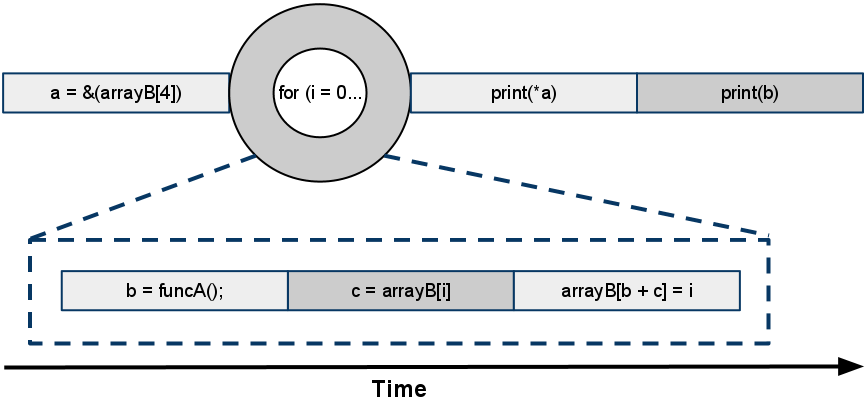
\includegraphics[width=6in]{images/ParallelTasksSequential}
\end{center}
\caption{Sequential Execution of Program in Figure~\ref{fig:parallelpseudosrc}}
\label{fig:parallelpseudoseq}
\end{figure}

Figure~\ref{fig:parallelpseudomedcntl} contains an illustractoin of
the execution of the pseudo-code in Figure~\ref{fig:parallelpseudosrc}
using medium-to-fine grained parallel tasks bounded by control flow
constructs.  This illustration assumes a static, likly points-to,
analysis finds that line 6 does not alter the heap locations read by
line 5.  Even if this is not the case, and line 5 depends on a value
written by line 6, it may still possible to create parallel software
pipelines~\cite{rangan:04:pact, giacomoni:08:ppopp}.

\begin{figure}
\begin{center}
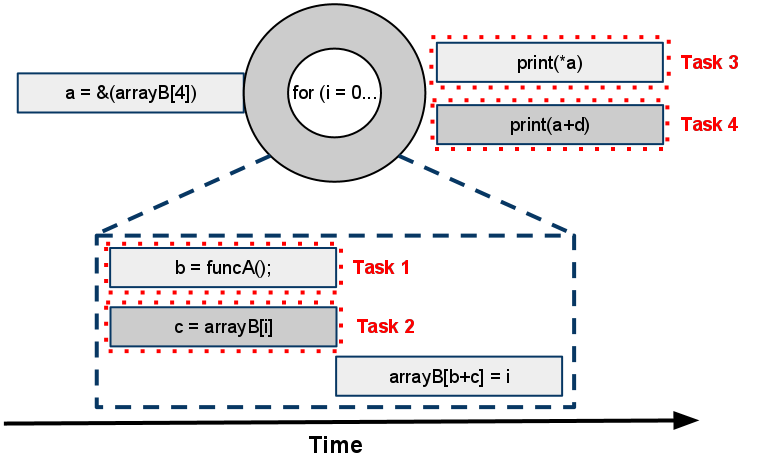
\includegraphics[width=5in]{images/ParallelTasksMedControl}
\end{center}
\caption{Static Fine-To-Medium Grained Parallel Tasks from Figure~\ref{fig:parallelpseudosrc}}
\label{fig:parallelpseudomedcntl}
\end{figure}

Figure~\ref{fig:parallelpseudosrc} demonstrates how the boundary of
parallel tasks located by static analysis can be limited by control
paths that are resolved at run-time~\cite{blume:1992:pds}.  Prior work
has found that even state-of-the-art automatic parallelizing compilers
are often unable to parallelize simple embarrassingly parallel loops
written in C/C++~\cite{minjang:10:micro}.

\subsection{Automatic Parallelization by Dynamic Analysis}

Dynamic auto-parallelization techniques examine the run-time execution
of a program, and thus can see how control flow dependencies are
resolved. This illustration in Figure~\ref{fig:parallelpseudocoarse}
show the pseudo-code in Figure~\ref{fig:parallelpseudosrc} could be
parallelized if a dynamic analysis were able to extract all potential
parallel instructions.  Note that the fine grained paralllel tasks
from Figure~\ref{fig:parallelpseudomedcntl} are still executed as
parallel tasks in Figure~\ref{fig:parallelpseudocoarse} spawned from
Task 2.

\begin{figure}
\begin{center}
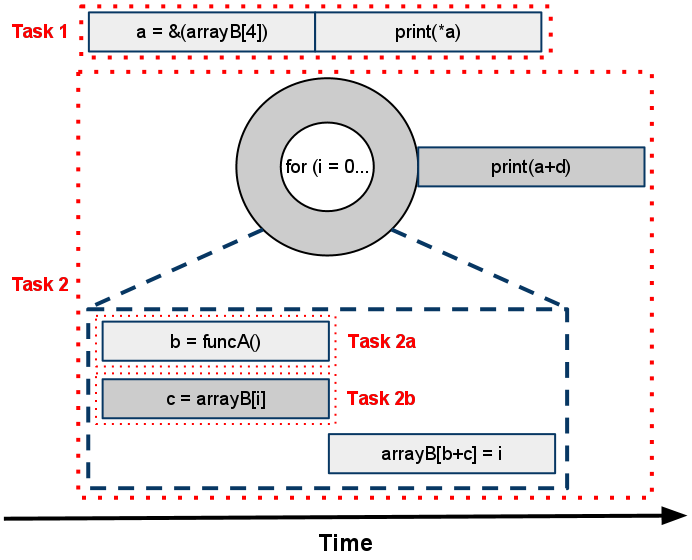
\includegraphics[width=5in]{images/ParallelTasksCoarse}
\end{center}
\caption{Static Fine-to-Coarse Grained Parallel Tasks from Figure~\ref{fig:parallelpseudosrc}}
\label{fig:parallelpseudocoarse}
\end{figure}

An illustraction of dynamic exection of the pseudo code in
Figure~\ref{fig:parallelpseudosrc} is shown in
Figure~\ref{fig:parallelpseudocoarsedyn}.  The \textit{for} loop from
the static code is shown partially unrolled in the the dynamic
exeuction illustration.

\begin{figure}
\begin{center}
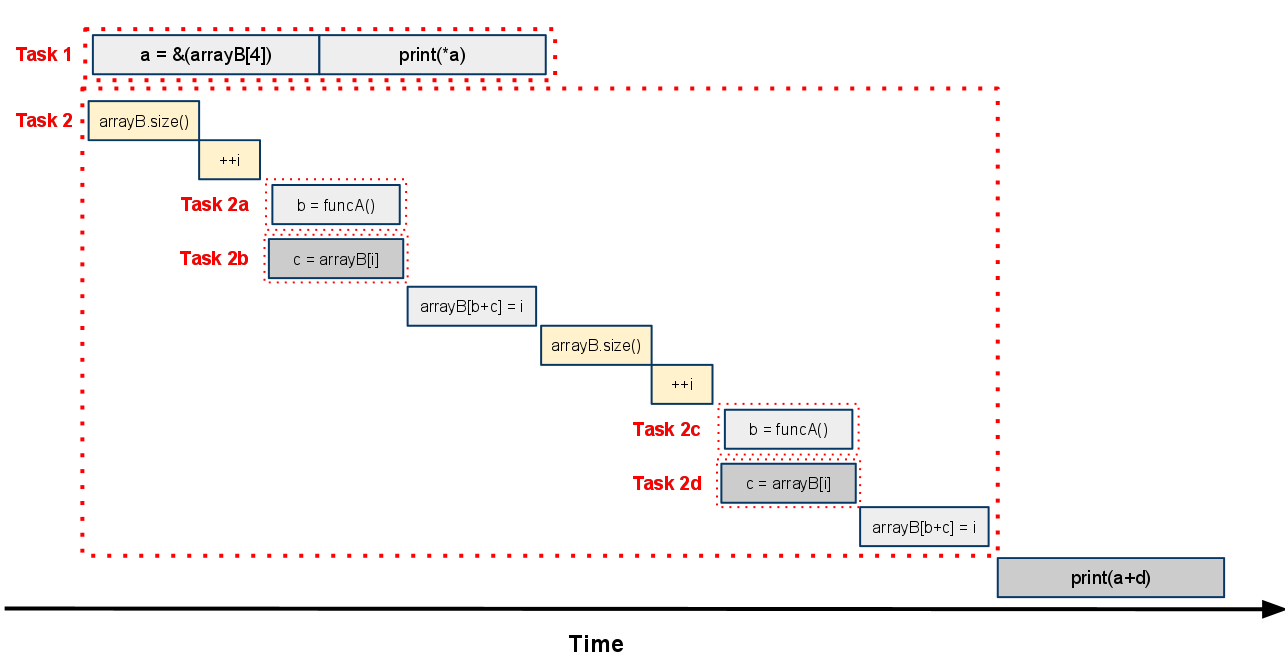
\includegraphics[width=5in]{images/ParallelTasksCoarseDyn}
\end{center}
\caption{Dynamic Coarse Grained Parallel Tasks from Figure~\ref{fig:parallelpseudosrc}}
\label{fig:parallelpseudocoarsedyn}
\end{figure}

Parallel tasks found by a dynamic analysis are only correct for the
program input, or the set of inputs, that have been analyzed.
Therefore, to ensure correct execution, thread-level parallelism found
and executed dynamically is often executed speculatively. There are
many works exploring thread-level speculative (TLS)
techniques~\cite{steffan:00:isca,vachharajani:07:pact,warg:2001:pact,wu:2008:cdp,chen:cc:2004,dou:2007:trans,wang:2009:dps,Rangan:2004kx,Ottoni:2005uq}.
This thesis does not require a detailed understanding of transactions
and speculation, but basic concepts are necessary.  If two tasks are
executed speculatively, then, for this work, it is assumed that the
program executed in such a way that the final program state is
identical to that of the sequentially executed code.

The illustration of the pseudo code in
Figure~\ref{fig:parallelpseudosrc} contains the dynamic code execution
with TLS from Figure~\ref{fig:parallelpseudocoarsedyn}.  The regions
of this illustration contained by \textit{Transaction 1} or
\textit{Transaction 2} may be rolled back by our hypothetical TLS
system.  Note that this illustration does not include nesting TLS;
this is also true for many research TLS
systems~\cite{prabhu:2005:ppopp}.

\begin{figure}
\begin{center}
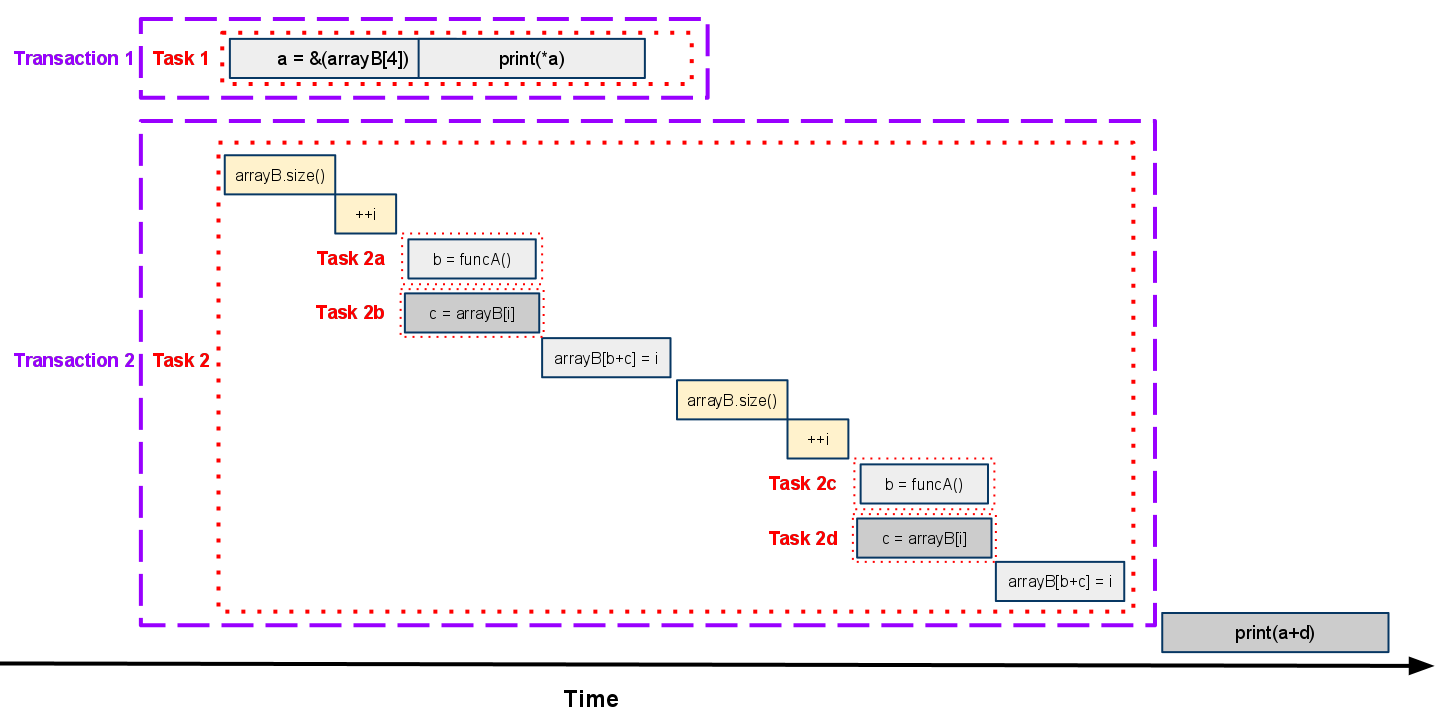
\includegraphics[width=5in]{images/ParallelTasksCoarseTLS}
\end{center}
\caption{Dynamic Coarse Grained Parallel Tasks from Figure~\ref{fig:parallelpseudosrc} with TLS}
\label{fig:parallelpseudocoarsetls}
\end{figure}

TLS often incorporate prediction to extract additional
parallelism~\cite{kejariwal:2007:tap}.  Prediction systems used by TLS
can speculate values, control directions, and data dependencies.
Figure~\ref{fig:parallelpseudocoarsepredtls} shows an illustration of
a TLS system using control prediction to execute each iteration of the
\textit{for} loop in parallel.  Value prediction in
Figure~\ref{fig:parallelpseudocoarsepredtls} also allows the value of
\textit{i}, which is read by instructions inside the \textit{for}
loop, to be predicted and propagated.

\begin{figure}
\begin{center}
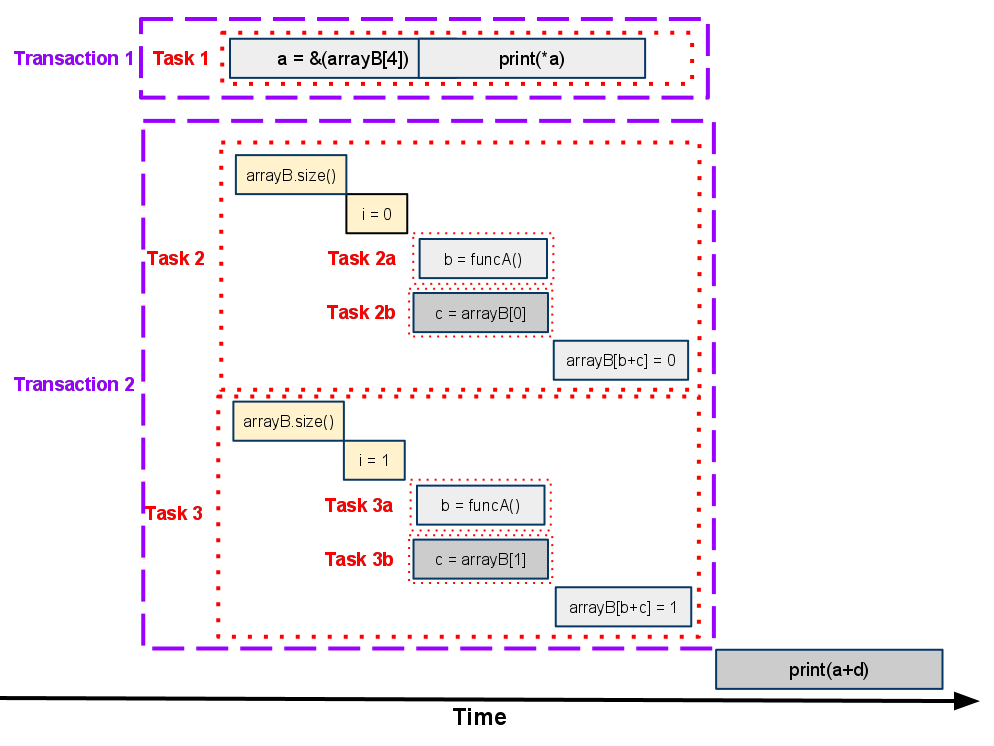
\includegraphics[width=5in]{images/ParallelTasksCoarsePredTLS}
\end{center}
\caption{Dynamic Coarse Grained Parallel Tasks from Figure~\ref{fig:parallelpseudosrc} with TLS and Prediction}
\label{fig:parallelpseudocoarsepredtls}
\end{figure}

The illustration in Figure~\ref{fig:parallelpseudocoarsetls} can help
explain why TLS is often most effective when extracting threads with
fewer than 1000 instructions~\cite{marcuello:00:ipdps}.  TLS will
often execute many iterations of If any instruction in \textit{Task 2}
conflict, then \textit{Transaction 2} will likely roll back the entire
transaction.  Complex tasks may increase the risk of misprediction by
including more predicted values, dependencies, and branch
directions~\cite{marcuello:00:ipdps}. Work by Ravi~\textit{et. al.}
looks at a technique based on transactional memory to expand TLS to
coarse-grained threads, but is limited to scientific codes with
regular access patterns~\cite{ramaseshan:08:nc}. TLS has been applied
to C and Java objects that contain thousands of instructions, but work
by Warg \textit{et. al.} found limited gains were realized from
objects with more than 100 instructions~\cite{warg:2001:pact}.

TLS can greatly improve program performace, regardless of the
granularity limitations. For example, TLS performance gains from a TLS
system that uses perform control, data dependence, and data value
speculation~\cite{kejariwal:2007:tap}, are shown in Figure
~\ref{fig:tlsperf}.

\begin{figure}
  \begin{centering}
    \begin{minipage}{\hsize}
      \begin{tabular}{ l c }
        Benchmark & TLS Perf \\
        \hline
        400.perlbench & 6.47 \\
        401.bzip2 & 12.31 \\
        403.gcc & 14.14 \\
        429.mcf & 17.7 \\
        445.gobmk & 12.78 \\
        456.hmmer & 0.1 \\
        458.sjeng & 16.1 \\
        462.libquantum & 0.1 \\
        464.h264avc & 3.34 \\
        471.ommnetpp & 15.5 \\
        473.astar & 40.67 \\
        483.xalancbmk & 9.1 \\
      \end{tabular}
    \end{minipage}
  \end{centering}
  \caption{Performance from TLS~\cite{kejariwal:2007:tap}}
  \label{fig:tlsperf}
\end{figure}

\section{Parallelization with Tools}
\label{sec:paralleltools}

Automatic parallelization is difficult, and most successes are limited
to highly numeric
applications~\cite{larus:1993:pads,ramaseshan:08:nc}.  This section
examines tools that can help a programmer find potential parallel
tasks and find potential task conflicts.  Static parallelization tools
have had some success~\cite{kennedy:91:pads}, but are ultimately
limited in the presence of pointers and dynamic memory
allocation~\cite{minjang:10:micro}. This section explores tools that
use run-time program information, much like TLS, for finding potential
parallel tasks and task conflicts.

Commerical applications that use dyanmic information to help find
potential parallelism generally keep the science behind these systems
a secret~\cite{cogswell:2010:eweek, vectorfabrics:11:ws}.  A limited
number of tools have recently emerged from the research community, and
are easier to explore for this section.

Alchemist is a dynamic profile based tool that deterimines potential
parallizable regions at runtime.  Dependence conflicts are also
located and presented to a user for manual
parallelization~\cite{zhang:09:cgo}.  The Alchemist tool restricts
parallel tasks to regions bounded by artifical constructs, like
if-than-else branches or loops.

Many tools that use dynamic program information to aid parallel
programming bound parallel tasks to artificial constructions that are
present in the static code during analysis~\cite{zhang:09:cgo,
  minjang:10:micro, jeon:2011:hotpar, garcia:2011:pldi}.  This
limitation is likely in place for the following reasons: 1), it is
unclear how to find task boundaries without constructs, 2) constructs
help trace compression, and 3) hot code blocks are often contained inside
loops.

Artifical constructs are an easy way to define a parallel task
boundries.  to First, it is unclear how to define the boundaries of
parallel tasks~\cite{jeon:2011:hotpar, garcia:2011:pldi} without
constructs.

prior works have found only limited benefit
when looking outside of constructs like \textit{for} loops or
\textit{if} statements~\cite{rinard:93:computer,rul:2008:sc}.Using
arti

The SD3~\cite{minjang:10:micro} tool performs inter-region dependence
analyses similar to those discussed in this work.  The regions located
by SD3 are defined stride-compression, and therefore are generally
limited to locating potential parallelizable regions in loops.  Many
recent advances in parallel task boundary locations are also limited to
parallelism bounded by explicit constructs~\cite{jeon:2011:hotpar,
  garcia:2011:pldi}.

This thesis presents a system for finding, analyzing, and extracting
potential parallel regions from serial codes.  The tool presented by
this thesis can be used to quickly develop dynamic traces analyses.
The trace compression developed for this thesis allows for off-line
analysis, thereby allowing new analysis to quickly be tested and
executed on a benchmark suite, without the additional step of
re-running each benchmark.  In fact, the ability to quickly develop new
analysis allows this system to be rapidly adapted to new tasks, such
as finding irrelevant code in dynamic traces.  For modern multicore
systems, the work in this thesis can find parallel tasks outside of
artificial constructs at a granularity of hundreds to millions of
instructions.

%%%%%%%%%%%%%%%%%%%%%%%%%%%%%%%%%%%%%%%%%%%%%%%%%%%%%%%%%%%%%%%%%%%%%%%%%%%%%
\chapter{Related Works}
\label{chap:background}
%%%%%%%%%%%%%%%%%%%%%%%%%%%%%%%%%%%%%%%%%%%%%%%%%%%%%%%%%%%%%%%%%%%%%%%%%%%%%

This chapter presents work relevant to this thesis.  Trace
compression, visualization, and analysis are examined in this chapter.
Decision diagram (DD) construction techniques are also discussed.

\section{Dynamic Trace Compression}

Managing large dynamic traces is the key problem when performing whole
program analyses. Consider that 1 billion 64bit values need $\approx$
7.5~GB of uncompressed storage and that traces usually contain
billions of instructions~(10-1000s of GB). Therefore, any trace
analysis tool must operate on compressed data. Further, analyzing this
data many need either sequential or random access mandating
different compression techniques. ParaMeter requires rapid random
access coupled with good compression.

Researchers have used three methods to reduce trace sizes: (1)
abstraction; (2) compression by predictor-based encoding; and, (3)
compression by program structure exposing methods, such as run-length
encoding or hierarchical grammars.  Stride-based compression
techniques have recently emerged as a viable option for some analyses,
such has hot-code and memory-conflict
location~\cite{minjang:10:micro}.

\subsection{Abstraction and Elimination}

Data abstraction creates an abstract representation for concrete data.
Abstract representations can be more compact and easier to analyze.
For example, some abstractions applied to concrete dynamic trace data
include, but are not limited to, a mapping from instructions to object
creation/destruction~\cite{sridharan:07:pldi}, or program
slices~\cite{zhang:04:icse}.

Data elimination removes information from a trace that is deemed
unnecessary by the original analysis designer.  For example, the whole
program path (WPP) trace representation~\cite{larus:99:pldi}
aggregates data from multiple occurrences of the same program
path.  However, information that is difficult to aggregate, like cache
misses or CPU temperatures, will be removed from the WPP
representation.

\subsection{Sequitur Compression}

The Sequitur compression algorithm is useful for compressing
instruction level dynamic traces into an analyzable
representation~\cite{manning:97:dcc}.  However, while Sequitur can
rapidly provide an analysis with information about the instruction
sequences in a trace, specific instruction information often requires
an expensive traversal of the grammar.  Do demonstrate grammar
creation, lets generate a grammar for the following sequence of
letters:
$$
abcdabcdabc
$$
We begin by creating a start rule:
$$
S \rightarrow abcdabcdabc
$$
Sequitur forms a grammar online, thus the algorithm would first detect the repetition of the variables $ab$.  The algorithm then creates a new rule $A \rightarrow ab$:
$$
\begin{array}{lcll}
S \rightarrow AcdAcdAc\\
A \rightarrow ab\\
\end{array}
$$
This processes is repeated for $Ac$, thereby forming a hierarchical grammar:
$$
\begin{array}{lcll}
S \rightarrow BdBdB\\
A \rightarrow ab\\
B \rightarrow Ac\\
\end{array}
$$
This processes is repeated for $Bd$:
$$
\begin{array}{lcll}
S \rightarrow CCB\\
A \rightarrow ab\\
B \rightarrow Ac\\
C \rightarrow Bd\\
\end{array}
$$

\subsection{Sequential Compressed Traces}

Burtscher \textit{et. al.}~\cite{burtscher:05:cgo} in 2005 described a predictor
based strategy requiring only mispredictions to be stored in the trace
file. The resulting compressed trace file is further compressed with a
standard stream compressor such as gzip or bzip2 achieving a 10 times
compression factor with rapid streaming decompression. Generating
interactive DINxRDY plots from such stream compressed data is
impractical as the data must be entirely decompressed for each frame,
$\approx 1$ minute on a 2.0~GHz Pentium 4 for each 800x600 pixel
plot in a trace containing only 100~million instructions.  Worse,
selecting and performing slice analysis on instructions requires two
additional passes through the complete data set adding another 2
minutes to the frame's render time.

Work by both Iyer \textit{et. al.}~\cite{iyer:05:epic} and Zhang et
al.~\cite{zhang:04:icse} addresses this problem by generating
intermediate representations. Iyer's work maintains a stream
compressed intermediate representation suitable for working on the
current frame, but leaves the navigation problem unsolved.  Zhang et
al.~\cite{zhang:04:icse} use a BDD to maintain the \textit{intermediate
  analysis} results in a compact form in RAM. However, the navigation
problem, as well as inquiries into the contents of a DINxRDY plot, is
still prohibitively expensive.

\section{Reduced Ordered Binary Decision Diagrams}
\label{sec:robdds}

Reduced, ordered, binary decision diagrams (BDD) were first described
by Akers~\cite{akers:78:itc} and further developed by
Bryant~\cite{bryant:86:ieeetc}.  BDDs have been used in many domains
including hardware verification~\cite{brayton:96:cav},
cryptography~\cite{krause:02:ec}, static program
analyses~\cite{whaley:05:pods,whaley:04:pldi}, and some use in dynamic
trace analysis~\cite{zhang:04:icse}.

\begin{figure}
  \centering
  \subfigure[Binary Decision Tree]{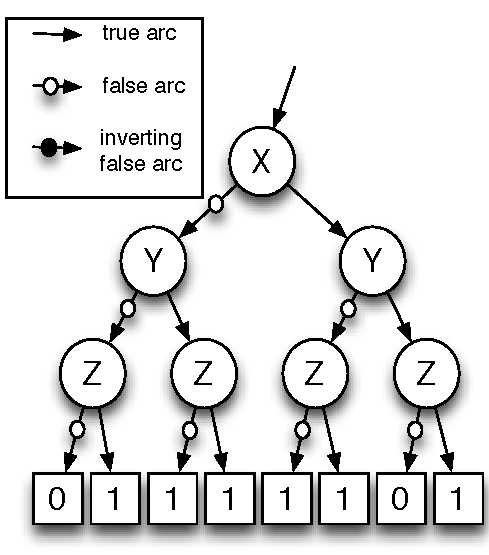
\includegraphics[height=2.50in]{figures/bdtree}}
  \hspace{5mm}
  \subfigure[Na\"ive Order]{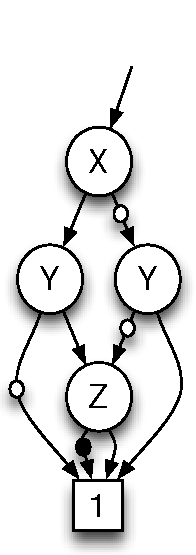
\includegraphics[height=2.50in]{figures/robdd}}
  \hspace{5mm}
  \subfigure[Better Order]{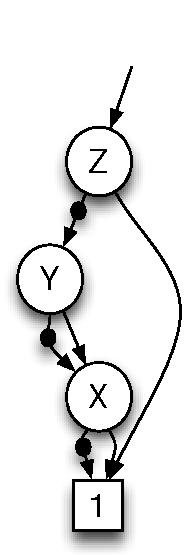
\includegraphics[height=2.50in]{figures/reorderbdd}}
  \hspace{5mm}
  \caption{A Three-variable Binary Decision Tree and BDDs} 
  \label{fig:bdtree}
  \label{fig:reorderbdd}
  \label{fig:robdd}
\end{figure}

BDDs can be viewed as compressed versions of binary decision trees.
Figure~\ref{fig:bdtree}(a) shows a binary tree for the three variable
function $f(x,y,z) = x'y + xy' + z$.  For example, traversing the left
edges of the graph we evaluate $f(0,0,0)$ as $0$.  BDDs are a graph
data structure in which each node corresponds to a Boolean function
(just as each node in a binary decision
tree)~\cite{bryant:86:ieeetc}. The following two reduction rules are
used to convert a decision tree to an BDd:

\begin{enumerate}

\item When two BDD nodes \textit{p} and \textit{q} are identical, edges
  leading to \textit{q} are changed to lead to \textit{p} and \textit{q} is
  removed

\item If both edges from a node \textit{p} go to 
  child node \textit {q}, then \textit{p} is eliminated and all nodes that
  go to \textit{p} are redirected to \textit{q}.

\end{enumerate}

The last reduction rule is commonly referred to as the
\emph{S-deletion}
rule~\cite{minato:01:STTT}. Figure~\ref{fig:robdd}(b) shows the BDD
for $f$ under the variable ordering~$(x,y,z)$ with additional
compression provided by inverting edges. To compute $f(0,0,0)$ with
the BDD, we traverse the $0$, or false, arc of the X node, the false
arc of the rightmost Y node and the inverting false arc of the Z node.
Because we reached the constant $1$ node through an odd number of
inverting arcs, we find $f(0,0,0)=0$ as before.

\section{Zero-Suppressed Binary Decision Diagrams}

For this research I propose using BDDs to represent sets of dynamic
program trace information.  The Boolean function that describes the
inclusion of a set in a Boolean function is called the
\textit{characteristic function}. BDDs can perform many set operations
efficiently~\cite{bryant:86:ieeetc}.  

However, Minato~\cite{minato:93:dac} found that BDDs were inconvenient
for sets of binary vectors.  The tuple based dynamic trace encoding
method used by this proposal employs a variation of this binary vector
encoding technique.  Specifically, a Minato creates sets of
combinations of objects represented by a binary vector,
$(x_{n}x_{n-1}x_{n-2}...x_{2}x_{1})$.  In this vector each bit
represents the inclusion of the object in the set.  Using BDDs, each
bit in the binary vector and a variable in the Boolean formula.  The
size of a BDD depends on the number of variables in the encoding, as
well as the variable order.  Therefore, it is useful to know the
smallest number of relevant bits in a bit vector before performing BDD
encoding.  Unfortunately, it is not always possible to know the
smallest number of relevant bits for a bit vector.

The following example better illustrates this problem: The vector
${0101}$ has four bits.  If the rightmost bit is the least significant
bit, then, in this case, let us assume only the rightmost three bits
are actually useful.  It is possible to encode this vector in a BDD
with three variables, representing the vector ${101}$.  However,
imagine this operation ${101} \wedge {1101}$. The BDD must not contain
four variables, but Boolean algebra states the vector ${101}$
contains a \textit{don't care} value for the fourth bit, which is not
correct.  Thus, the BDD should be built with a variable for each
potential bit in the bit vector.

Minato~\cite{minato:93:dac} proposed a variation on BDDs, called ZDDS,
to address this issue, and to reduce the size of BDDs for sparse data
sets.  ZDDs are a variant of BDDs where the \textit{S-deletion}
compression rule is replaced by the use of the \emph{pD-deletion}
compression rule.  In this section we see that ZDDs provide better
compression than BDDs for trace data, and over $9\times$ faster
creation times.

Zero-suppressed BDDs, or ZDDs, replace the \textit{S-deletion} rule with
the \textit{pD-deletion} rule.  This rule states the following:
\begin{itemize}

\item If the \textit{1} edge from a node \textit{p} leads to a zero
  terminal node and whose \textit{0} edge a child node \textit {q}, then
  \textit{p} is eliminated and all nodes that lead to \textit{p} are
  redirected to \textit{q}.

\end{itemize}

Furthermore, ZDDs do not typically implement the inverting arcs
optimization, i.e., ZDDs have no inverting arcs, only plain $then$ and
$else$ arcs.  To see how this rule change results in a different
decision diagram, consider, once again, the function $f(x,y,z)$ whose
binary decision tree was shown in Figure~\ref{fig:bdtree}a.
Figure~\ref{fig:rozdd} shows the ZDD for this function.
\begin{figure}
  \centering
  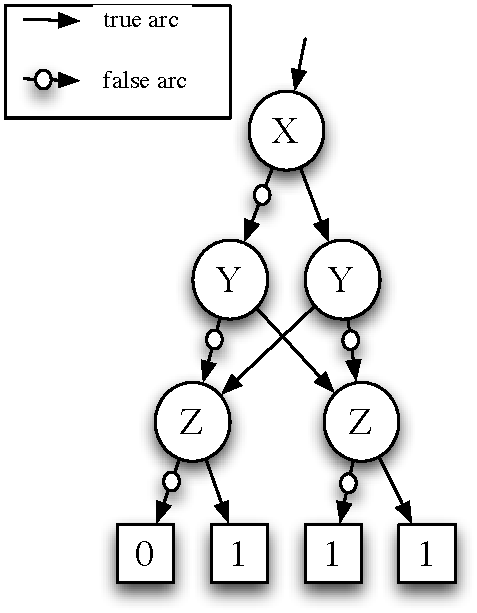
\includegraphics[height=2.5in]{figures/rozdd}
  \caption{A ZDD for $f(x,y,z)$}
  \label{fig:rozdd}
\end{figure}
For this function, ZDDs perform worse than BDDs, as most of the values
for $(x,y,z)$ cause the function to evaluate to 1.  However, for
sparse functions (i.e., those with few 1's in the range), such as
trace data, ZDDs provide superior compression.

\section{Hot Code Analysis}

Ammons \textit{et. al.} found that hot code regions often occupy less than 28\%
of the overall program code, resulting in up to 98\% of level one cache
misses~\cite{ammons:97:sigplan}.  Therefore, hot code information can
tell programmers where to focus parallelization efforts.  Using
Sequitur-based trace representations, hot path information can be
generated by recursively summing the number of occurrences of
sub-rules in a grammar~\cite{larus:99:pldi}.


\section{Dynamic Trace Analysis}
\label{sec:dynanalysis}

Dynamic traces information consists of information collected from a
program at run-time.  Software developers can use instruction level
dynamic trace analyses to create a picture of their software's
run-time behavior, as well as software
debugging~\cite{zhang:04:micro}.  However, dynamic traces can grow
quickly in size (gigabytes to terabytes) for seconds of program
execution. Analysis of large quantities of data can be impractical
using commodity hardware~\cite{reiss:01:icse}.

\section{DINxRDY Visualizations}
\label{sec:dinrdyplots}

Though parallelism found in prior studies~\cite{lam:92:isca,
  wall:93:decwrl, austin:92:isca} is not accessible to ILP
techniques~\cite{wall:93:decwrl}, it may yield to thread level
parallel (TLP) techniques.  The Dynamic Instruction Number
vs. Ready-time~(DINxRDY) plot (originally introduced by Postiff et
al.~\cite{postiff:98:um}) can be useful in identifying the potential
TLP inherent in many sequential applications.

\begin{figure}
  \begin{center}
  	\subfigure[As Captured]{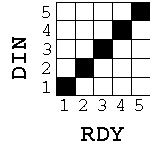
\includegraphics[width=1.5in]{figures/ex_dinxrdy_1}}
	\hspace{.9in}
  	\subfigure[Ideal Schedule]{\hspace{.1in}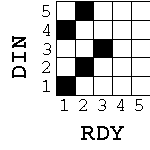
\includegraphics[width=1.5in]{figures/ex_dinxrdy_2}\hspace{.1in}}
  \end{center}
  \caption{Basic DINxRDY Plot with 5 instructions.}
  \label{fig:ex_dinxrdy}
\end{figure}

DINxRDY plots graphically represent parallel structures and
expose potential threads for TLP~\cite{iyer:05:epic}.  Consider the
hypothetical 5 instruction trace shown in
Figure~\ref{fig:ex_dinxrdy}(a).  The vertical axis represents the
Dynamic Instruction Number~(DIN) and the horizontal axis represents
the earliest time at which an instruction can be
scheduled~(ready-time, RDY).  For example,
Figure~\ref{fig:ex_dinxrdy}(a) shows that the 3rd instruction in the
trace (dynamic instruction 3, or DIN 3) was issued in cycle 3.
Figure~\ref{fig:ex_dinxrdy}(b) shows the same trace under an ideal
schedule (i.e., one cycle per instruction, perfect branch
prediction, infinite hardware resources, etc.) that respects all data
dependencies.  This plot shows that DIN~3 is dependent on DIN~2 which
in turn is dependent on DIN~1.  Further, the plot shows that DIN~4
is not dependent on DINs 1, 2, or 3 because it is scheduled in the
first cycle.  Dependency analysis is needed to decide whether DIN~5 is
dependent on DIN~1 or 4.

Iyer \textit{et. al.} observed that lines running from lower left to
upper right in DINxRDY plots form dependency chains of relatively
nearby instructions in a program~\cite{iyer:05:epic}.  Further,
diagonal lines that have overlapping x-extents suggest regions of code
that might be convertible to TLP. Figure~\ref{fig:sampledinvrdy} shows
a DINxRDY plot for 254.gap with groups of divergent dependency
chains~(DDCs) (circled in the figure) suitable for TLP extraction
analysis. From Iyer's work~\cite{iyer:05:epic}, we know that these
suggest the presence of either data parallelism or pipeline
parallelism.

%% \begin{figure}
%% \begin{center}
%% \begin{picture}(0,0)
%% 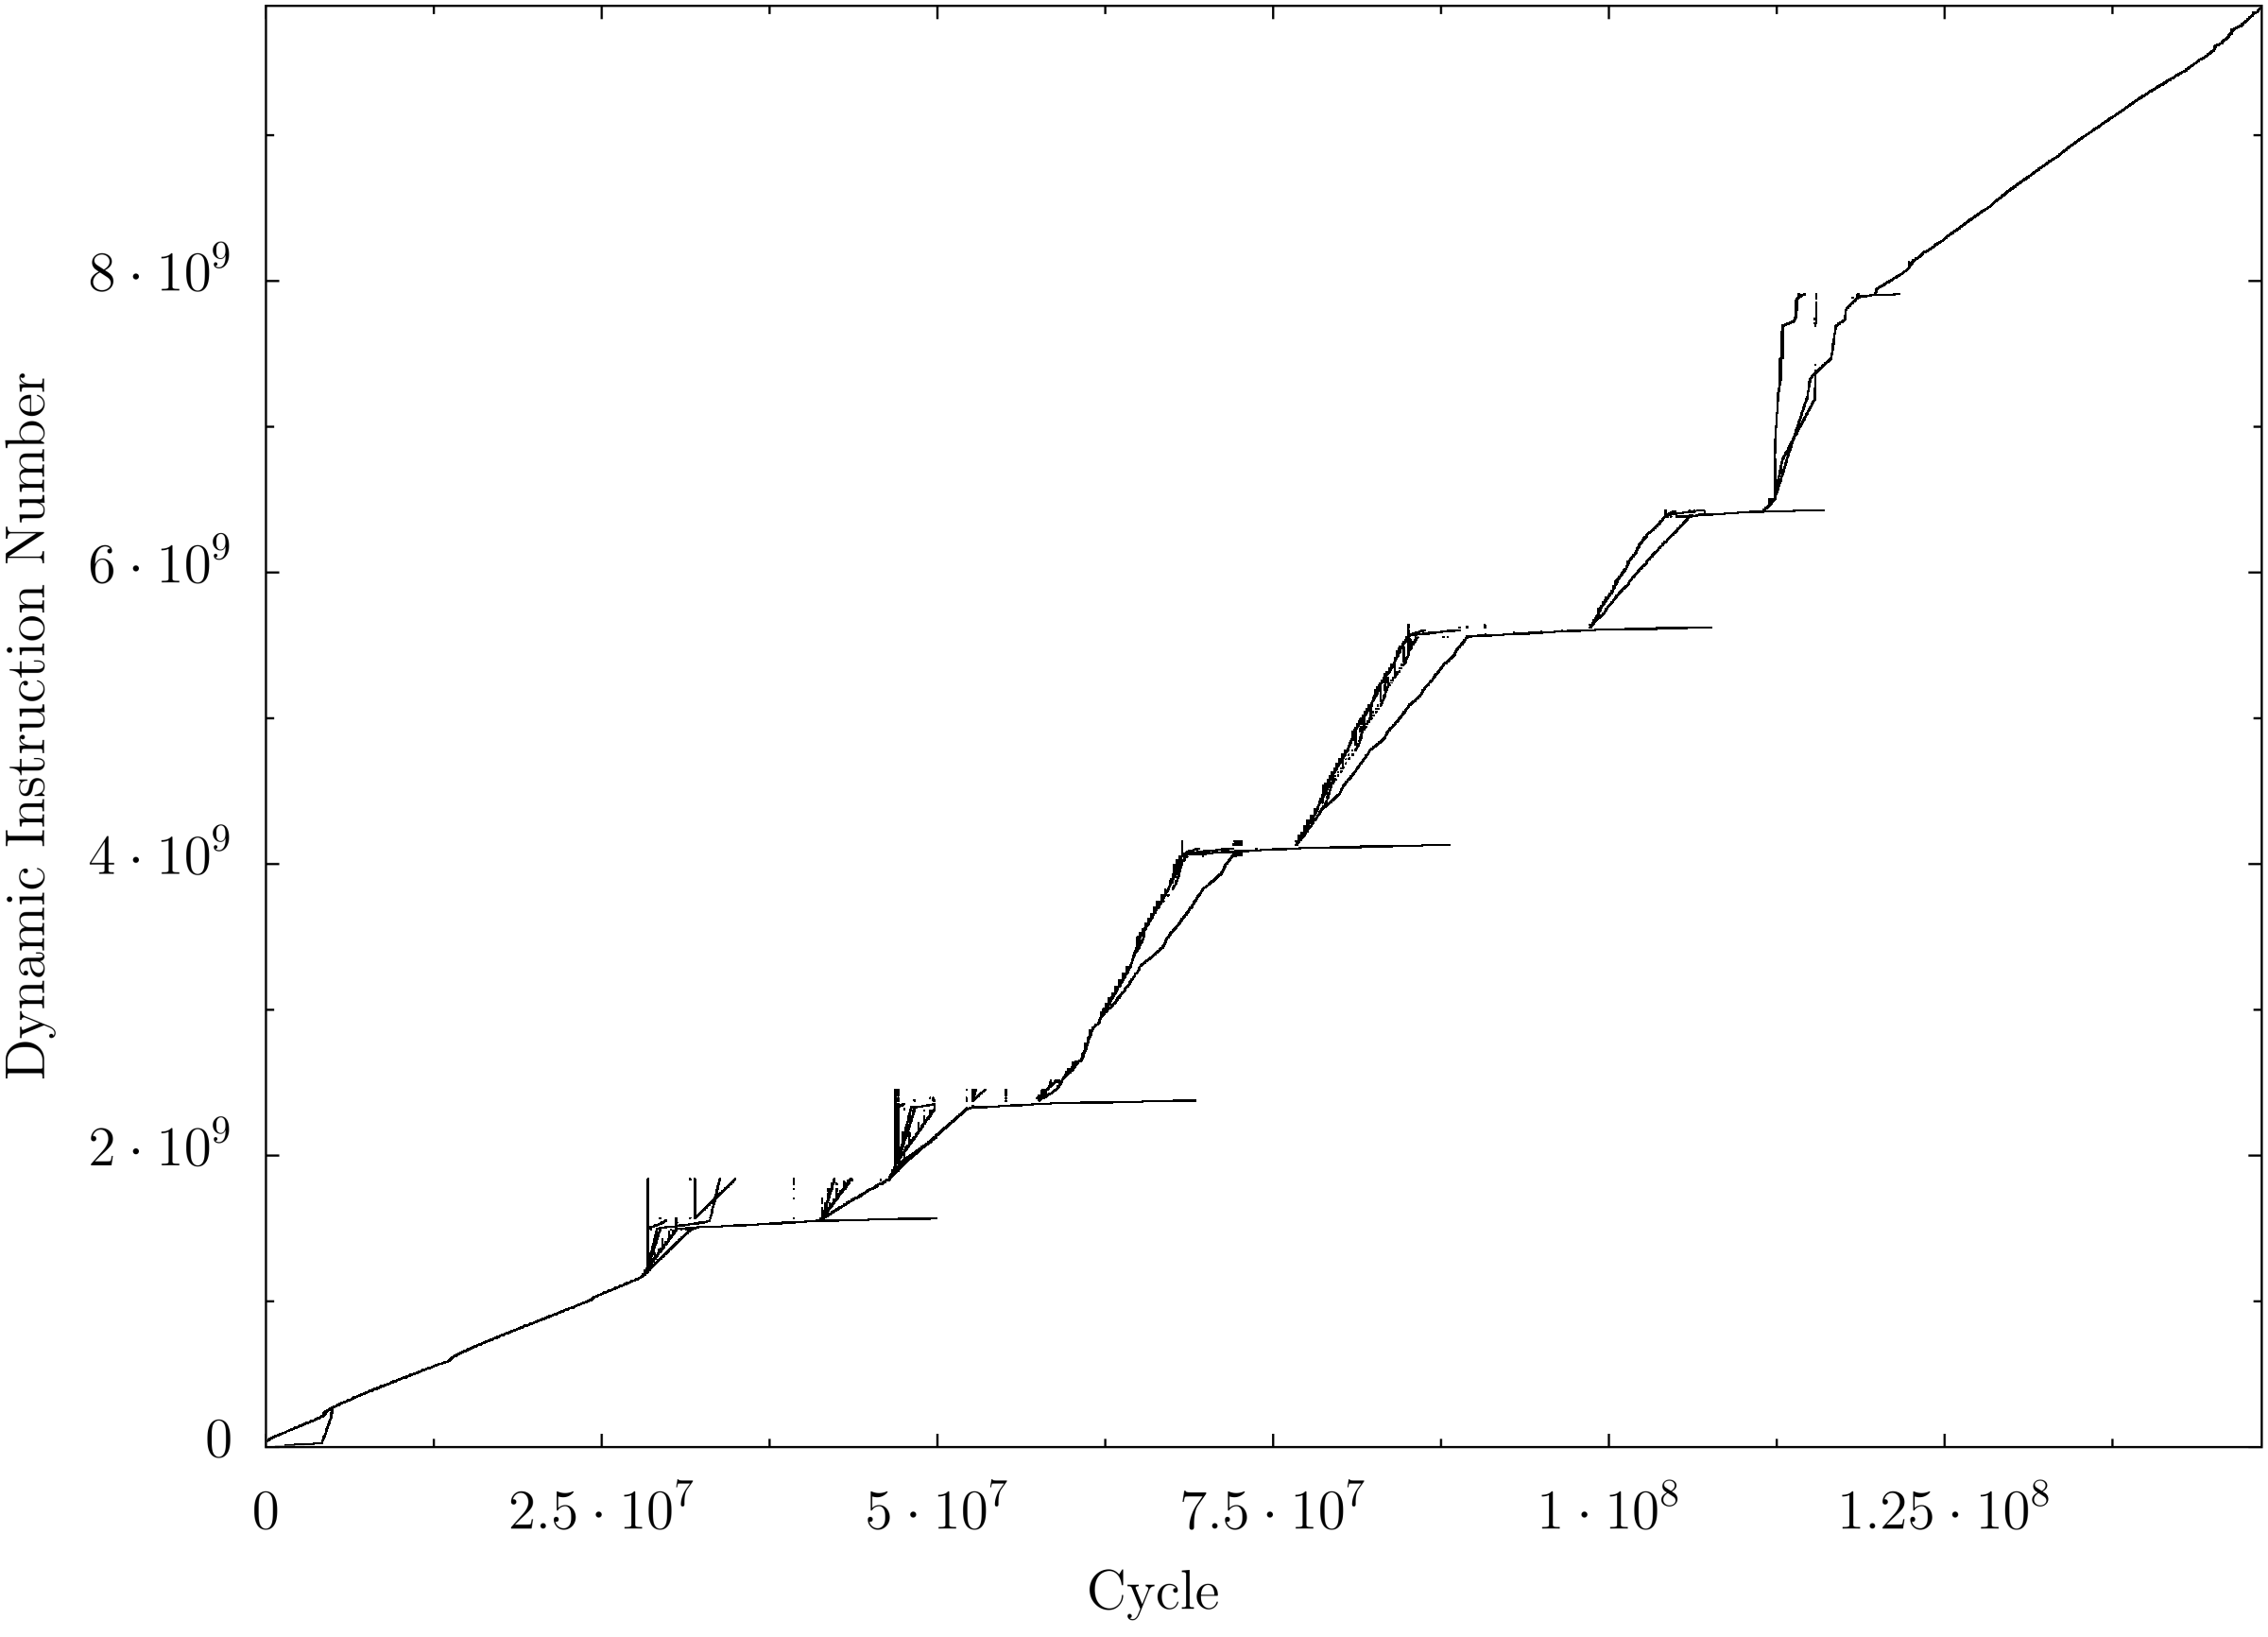
\includegraphics[width=3in]{figures/ia64_254_gap_gcc_inf_bw_din_crop2}
%% \end{picture}
%% \begin{picture}(225,155)
%% \put(85,49){\circle{20}}
%% \put(129,87){\circle{30}}
%% \put(160,42){\vector(-2,3){20}}
%% \put(160,42){\vector(-1,0){64}}
%% \put(140,35){\makebox(48,3){\tiny{Dependency chains (potential threads)}}}
%% \end{picture}
%% \end{center}
%% \caption{Dynamic instruction number vs. ready-time plot of SPEC INT 2000 benchmark 254.gap.  Circled areas represent potential threads}
%% \label{fig:sampledinvrdy}
%% \end{figure}

\begin{figure}
\begin{center}
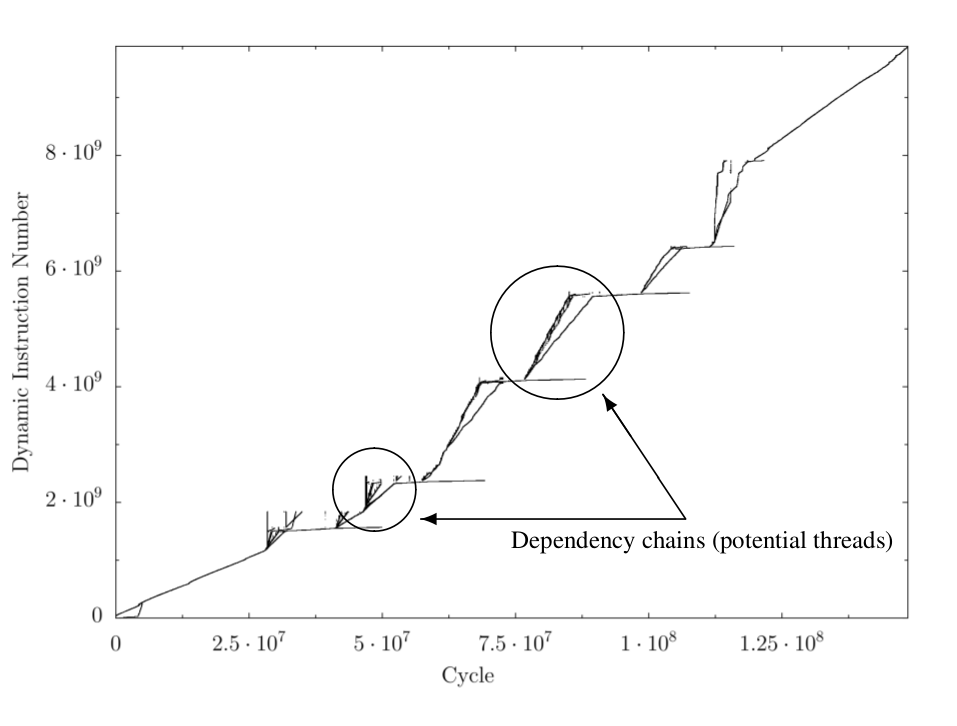
\includegraphics[width=4.5in]{images/dinrdyexample}
\caption{Dynamic instruction number vs. ready-time plot of SPEC INT 2000 benchmark 254.gap.  Circled areas represent potential threads}
\end{center}
\label{fig:sampledinvrdy}
\end{figure}

The Dynamic Instruction Number vs. Ready-time~(DINxRDY) plot
(originally introduced by Postiff \textit{et. al.} in 1998~\cite{postiff:98:um})
can be a useful in identifying the potential TLP inherent in many
sequential applications.  The dynamic instruction number (DIN) is a
unique number assigned to each instruction when the instruction
executes at run-time.  A single static instruction can execute many
times during program execution and each occurrence of that static
instruction would generate a new DIN.  The relation from $SIN
\rightarrow DIN$ is also stored.

This thesis uses sets $\{DIN_{i}, \{DIN_{d}\}\}$ for program analysis.
The $DIN_{i} \rightarrow \{DIN_{d}\}$ relation, also referred to as
{DINxDIN} in this thesis, maps an instruction $DIN_i$ to a set of
instructions $DIN_{d}$.  The members of the set $DIN_{d}$ have a
dependency that is resolved by dynamic instruction $DIN_i$.  Thus, it
is possible to use the $DIN_{i} \rightarrow DIN_{d}$ to identify
dependency relationships and perform dependence slicing. A full list
of ZDD trace tuple types can be found in
Appendix~\ref{appdx:tracetypes}.

\subsection{Dynamic Program Slicing}

Numerous works have used dynamic program trace slicing, introduced by
Korel \textit{et. al.}~\cite{korel:88:ipl}, to explore program
behavior at run-time.  Dynamic slices have been developed for locating
the source of observed program bugs~\cite{tip:94:cwi,agrawal:90:pldi},
program testing~\cite{gallager:91:se} and software
maintenance~\cite{kamkar:93:sm}. Dynamic traces can quickly grow in
size beyond what can be stored and analyzed on commodity
hardware~\cite{agrawal:90:pldi, zhang:04:micro, price:06:cal}.
Generating slices from large dynamic traces can require days of
computation time~\cite{agrawal:90:pldi}.  To reduce slice times, this
thesis extends the prior use of dependence
chopping~\cite{gupta:2005:ase,krinke:2004:sqc}.

Zhang \textit{et. al.} first explored slicing with
BDDs~\cite{zhang:04:icse}. In the work by Zhang, program slice
information for each instruction is generated from the dynamic trace
information. A variation of technique used to create program slices is
also used for the work in this thesis.

\subsection{Hot Code Analysis}

Hot code analysis can tell developers where to focus optimization and
parallelization efforts.  Ammons \textit{et. al.} found that hot code
regions often occupy less than 28\% of the overall program code,
resulting in up to 98\% of level one cache
misses~\cite{ammons:97:sigplan}.  Therefore, hot code information can
tell programmers where to focus parallelization efforts.  Using
Sequitur-based trace representations, hot path information can be
generated by recursively summing the number of occurrences of
sub-rules in a grammar. Using BDD-encoded traces, hot code information
is generated directly from the program execution by maintaining a
count of each static instruction's occurrence in the dynamic trace.

\section{Parallelism in Computing}
\label{sec:parallelism}

Until recently, software engineers could gain performance by waiting
for processor core performance to improve.  However, manufacturers
have been unable to extract performance from uni-processor designs,
forcing a trend towards multi-core systems~\cite{sutter:05:ddj}.
Tasks can be parallelized using a variety of scopes:

\begin{itemize}
\item System Parallelism
\item Application Parallelism
\item Thread Level Parallelism
\item Instruction Level Parallelism
\end{itemize}

With the advent of compute cloud infrastructures, tasks that may be
parallelized among systems can be expanded (or reduced) depending on
demand~\cite{nurmi:09:ccgrid}.  Application parallelism exists if
there is a need, or desire, to run multiple applications at the same
time on the same operating system.  Thread level parallel distributes
work between regions of the same program, with no programmer stated
total order between regions.  Programmers can state an explicit order
using synchronization methods such as locks, mutexes or
transactions~\cite{larus:tmbook:mcp:2006, gottschlich:10:cgo}.

Limit studies during the 1990s showed that sequential applications
have considerable potential parallelism~\cite{lam:92:isca,
  wall:93:decwrl, austin:92:isca, postiff:98:um} that is amenable to
thread level parallelism~(TLP)~\cite{iyer:05:epic} but is not
accessible via hardware instruction level parallel
techniques~(ILP)~\cite{wall:93:decwrl}. Therefore, the proposed
research will focus on software optimization through extraction of
thread level parallelism from existing sequential applications.



%%%%%%%%%%%%%%%%%%%%%%%%%%%%%%%%%%%%%%%%%%%%%%%%%%%%%%%%%%%%%%%%%%%%%%%%%%%%%
\chapter{Dynamic Trace Analysis at Scale}
\label{chap:scale}
%%%%%%%%%%%%%%%%%%%%%%%%%%%%%%%%%%%%%%%%%%%%%%%%%%%%%%%%%%%%%%%%%%%%%%%%%%%%%

\section{BDD Compression Time}
\label{sec:bddwork}

To understand why BDD-based compression is time consuming, this
section begins by first describing BDD-based trace
representation\cite{price:06:cal}. This section then analyzes the
BDD-trace creation algorithm and shows that inefficient trace BDD
compression is primarily caused by:

\begin{itemize}
\item Frequent garbage collection of dead BDD nodes
\item The deallocation of potentially reusable dead BDD nodes and
  corresponding BDD system cache entries
\end{itemize}

\subsection{Traces as Boolean Functions}

BDDs represent boolean functions, and thus, to represent traces as
BDDs, let us review how to represent trace data as a boolean
function~\cite{price:06:cal}.

Observe that boolean functions can encode arbitrary binary data.  For
example, if the represented universe, $\Omega$, consists of 4 elements
$\Omega = \{a,b,c,d\}$, then a 2-bit encoding can be used to represent
each element, $\{a \mapsto 00, b \mapsto 01, c \mapsto 10, d \mapsto
11\}$~\cite{price:06:cal}.  It is possible to create a boolean
indicator function (i.e., characteristic function) that evaluates to
true for any subset of the $\Omega$ with this encoding.  For example,
the indicator function for the set $\{a,b\}$ is $I_{\{a,b\}} = x'$
where $x$ is the variable for the most-significant bit (MSb) of the
set encoding and $x'$ is read as not $x$.

\newcommand{\DIN}{\ensuremath{\mathrm{DIN}}}
\newcommand{\PC}{\ensuremath{\mathrm{PC}}}

It is possible to extend this simple notion to encode different data
sets necessary for representing and analyzing the trace.  All trace
data is encoded by a set of tuples $(DIN,data)$ where the DIN is the
dynamic instruction number (i.e., the position in the trace, the first
instruction has DIN 0, the second DIN 1, and so on).  Therefore, a
simple instruction trace is encoded as $(DIN,PC)$, where the PC is the
program counter value. Similarly, more complex data relationships can
be encoded by simply joining the binary representations of arbitrary
tuples into a single equation.

This chapter uses three types of data tuples.  The first is
$(DIN,SIN)$, where the $SIN$ is the static instruction number or $PC$
(Note that this thesis will use $PC$ and $SIN$ interchangeably).  The
second tuple type is $(DIN,DIN)$, which is used to represent edges of
the trace's dynamic data dependence graph.  If a decision diagram (DD)
encodes an edge set $E$, if $(10,24)$ is in the edge set then the 24th
instruction in the trace depends on the 10th instruction in the trace.
If we wish to know the $PC$ of either of these instructions, we can
refer to the $(DIN,SIN)$ tuple set.  Finally, this thesis evaluates
$(DIN,RDY)$ tuple sets, which encode the ideal schedule for the trace,
i.e., for each $DIN$, $RDY$ is the earliest time a scheduler could
execute that $DIN$ given an ideal machine~\cite{price:08:pact}.  A
description of all tuple members and relation types can be found in
Appendix~\ref{appdx:tracetypes}.

\subsection{Boolean Functions as BDDs}

BDDs can be viewed as compressed versions of binary decision trees.
Figure~\ref{fig:bdtree}(a) shows a binary tree for the three variable
function $f(x,y,z) = x'y + xy' + z$.  For example, traversing the left
edges of the graph we evaluate $f(0,0,0)$ as $0$.  BDDs are a graph
data structure in which each node corresponds to a boolean function
(just as each node in a binary decision tree
does)~\cite{bryant:86:ieeetc}. A full discussion of BDD creation can
be found in Chapter~\ref{chap:background}, but for clarity the two
reduction rules for converting a decision tree to an BDD are:

\begin{enumerate}

\item When two BDD nodes \textit{p} and \textit{q} are identical, edges
  leading to \textit{q} are changed to lead to \textit{p} and \textit{q} is
  removed

\item If both edges from a node \textit{p} go to 
  child node \textit {q}, then \textit{p} is eliminated and all nodes that
  go to \textit{p} are redirected to \textit{q}.

\end{enumerate}

The last reduction rule is commonly referred to as the
\textit{S-deletion}
rule~\cite{minato:01:STTT}. Figure~\ref{fig:robdd}(b) shows the BDD
for $f$ under the variable ordering~$(x,y,z)$ with additional
compression provided by inverting edges. To compute $f(0,0,0)$ with
the BDD, we traverse the $0$, or false, arc of the X node, the false
arc of the rightmost Y node and the inverting false arc of the Z node.
Because we reached the constant $1$ node through an odd number of
inverting arcs, we find $f(0,0,0)=0$ as before. BDD creation is
covered in more detail in the
literature~\cite{somenzi:09:cu,bryant:86:ieeetc,price:06:cal}.

\subsection{BDD Unique Tables}

Prior work shows how to encode trace data as BDDs.  However, the
encoding processes can take an unreasonable amount of time.
Inefficient encoding is primarily caused by the interaction of garbage
collection and BDD system caches, specifically the unique table and
the operation cache.

The \textit{S-deletion} rule used to reduce a binary tree into a BDD is
realized through the \textit{unique table}.  The unique table enforces
strong canonicity because each new node has a unique location in the
table.  If a node is a duplicate of an existing table node (i.e., it
represents the same boolean function), the node is reused from the
unique table~\cite{bryant:86:ieeetc}. The unique table also increases
the efficiency of BDD creation.  If a BDD node already exists the BDD
management system, such as CUDD~\cite{somenzi:09:cu} (a state of the
art, high-performance, BDD package), saves time by reusing the
existing node and avoiding re-computation for the remainder of the
nodes below the cached one.

The unique table can be used to tune the overall creation time of the
BDD by altering its size.  The size of the unique table must at least
be large enough to contain all of the live BDD nodes.  With CUDD,
however, nodes contained in the subtable can also be dead. Upon
garbage collection, these dead nodes are added to \textit{death row},
which is an additional cache used to hold recently invalidated nodes.
The nodes on death row can also be resurrected and reused.

In addition to a simple node cache, BDD packages, including CUDD, also
have an operation cache that caches the results of BDD operations.
For example, if one requests a computation of $B \land C$ and the
result is $A$, then CUDD will cache that $A = B \land C$.  If $B \land
C$ is requested again, it will immediately return BDD $A$ from this
cache, and perform the potentially exponential recursion required to
recompute $A$.  This cache gives BDDs their polynomial time
complexity~\cite{bryant:86:ieeetc}.

Unfortunately, garbage collection frees the nodes on death row in
order to free memory, which, in turn, evicts corresponding results
from the operation cache.  As we will see, the eviction of useful
results caused by accumulation of real garbage ultimately hinders BDD
creation efficiency.

\subsection{Garbage Collection and Compression Time}

Garbage collection allows BDD packages to control memory consumption
and free the dead nodes on death row.  The CUDD package uses a
saturating reference counter to keep track of the amount of node use,
and to determine if a node is safe to delete.  A reference counting
system also aids other BDD functions related to automatic variable
ordering.  

CUDD uses plain pointers to \texttt{DdNode}s as a handle to an entire
BDDs.  If $A$, $B$, and $C$ have different pointer values they will
represent different BDDs.  In the pseudo code presented above, the $B$
and $C$ BDDs have their reference counts increased to prevent them
from being garbage collected.  $B$ and $C$ are then combined using a
boolean $\land$ operator to create the new BDD $A$.  $A$ then also has
its reference count increased to prevent garbage collection, but the
code now decreases the reference count of $B$ and $C$.  If $B$ and $C$
now have reference counts equal to zero they are considered
\textit{dead}, and could be removed by garbage collection.

To explain how BDD trace creation produces garbage, we first must
consider the BDD creation algorithm.  The algorithm is simple.  For
each tuple, a BDD is created to represent the single element tuple
(see the work~\cite{price:06:cal} for details), call it $E$, and this
BDD is OR'ed into the set of all tuples, call it $\Omega$.  The
pseudo-code for the algorithm using CUDD calls is shown in
Figure~\ref{fig:bddbuildset}.

\begin{figure}
  \begin{lstlisting}
    DdNode * buildSet()
    {
      DdNode *Omega = getEmptySetBdd()
      while(!done) {
        DdNode *OmegaOld = Omega;
        DdNode *E = getNextTupleBdd(); 
        Cudd_Ref(E);
        Omega = Cudd_or(OmegaOld, E);
        Cudd_Ref(Omega);
        Cudd_RecursiveDeref(E);
        Cudd_RecursiveDeref(OmegaOld);
      }
      return Omega;
    }
\end{lstlisting}
\caption{BDD Build Set}
\label{fig:bddbuildset}
\end{figure}

Notice that at the end of each loop iteration the only live nodes are
those that are part of the BDD for the current $\Omega$; all other
nodes are marked as dead.

Now, let us examine how this algorithm interacts with the BDD package
and its data structures.  Let us set $E =
\bar{X}\land\bar{Y}\land\bar{Z}$ which is exactly the shape of a tuple
BDD, assuming that we only had 8 possible tuples and thus 3 boolean
variables (in practice there are typically 64-128 variables per
tuple). In Figure~\ref{fig:bddtrace01} we can see the BDD
representation of the boolean function for $E =
\bar{X}\land\bar{Y}\land\bar{Z}$.

\begin{figure}
  \centering
  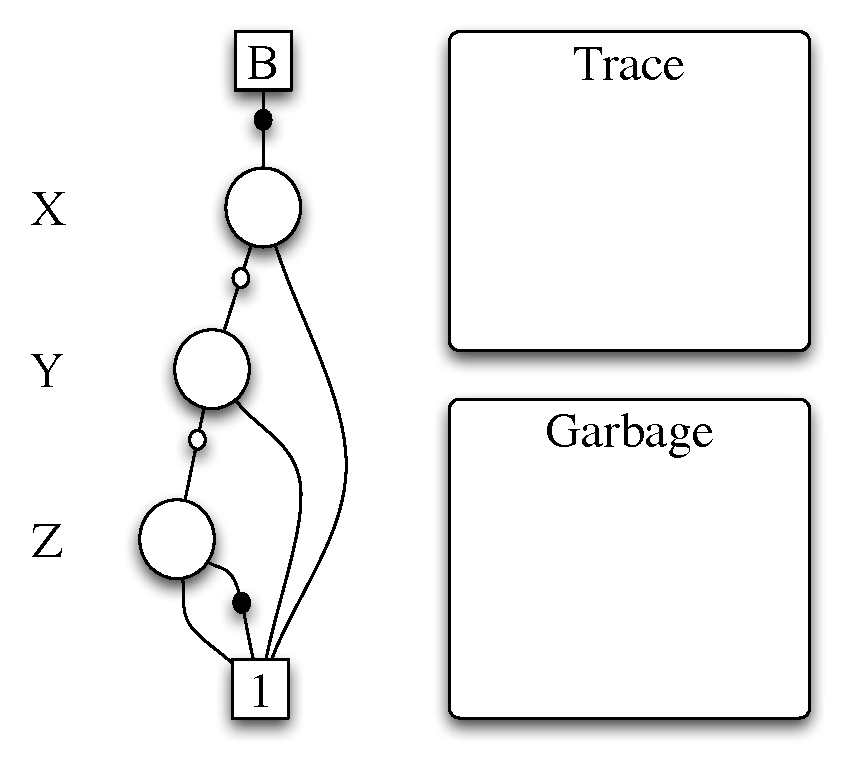
\includegraphics[height=2.5in]{figures/bddtrace01}
  \caption{A BDD for $\bar{X}\land\bar{Y}\land\bar{Z}$}
  \label{fig:bddtrace01}
\end{figure}

As shown in the Figure~\ref{fig:bddbuildset}, the start of the
algorithm initializes the trace BDD as empty.  After the BDD is
created for $E$, $E$ is added to the trace BDD by computing $\Omega =
E \lor 0$, as shown in the pseudo-code in
Figure~\ref{fig:bddbuildset}.

\begin{figure}
  \centering
  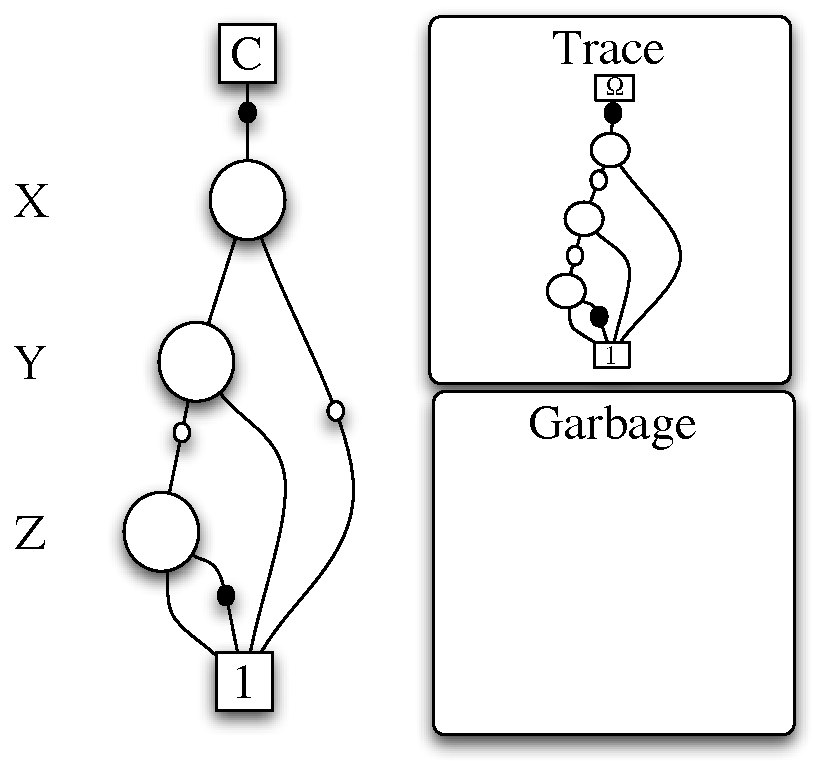
\includegraphics[height=2.5in]{figures/bddtrace02}
  \caption{A BDD for $(X\land\bar{Y}\land\bar{Z})$}
  \label{fig:bddtrace02}
\end{figure}

Now we need to add our second tuple to the set, call it $E'$.  The BDD
for $E'$ is shown in Figure~\ref{fig:bddtrace02} along with the BDD
for $\Omega$ and the garbage created so far. 

Figure~\ref{fig:bddtrace03} shows the trace BDD $\Omega$ after adding
$E'$.  In this new BDD, the $X$ term is now a \textit{don't - care}
value because the result of the function no longer depends on the
value of $X$.  The \textit{S-deletion} rule removes \textit{don't
  care} values from the BDD structure.  Figure~\ref{fig:bddtrace03}
shows the BDD for the function
$(\bar{X}\land\bar{Y}\land\bar{Z})\lor(X\land\bar{Y}\land\bar{Z})$
with the $X$ node removed.

\begin{figure}
  \centering
  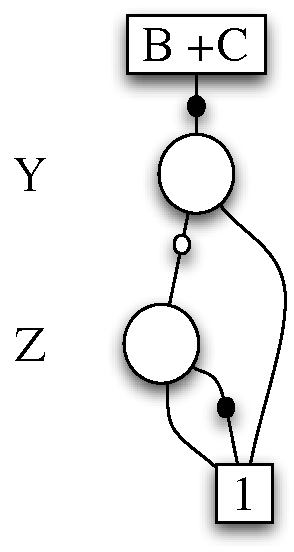
\includegraphics[height=2.5in]{figures/bddtrace03}
  \caption{A BDD for $(\bar{X}\land\bar{Y}\land\bar{Z})\lor(X\land\bar{Y}\land\bar{Z})$}
  \label{fig:bddtrace03}
\end{figure}

In Figure~\ref{fig:bddtrace04} we show yet another tuple $E'' =
\bar{X}\land\bar{Y}\land\bar{Z}$, which will be added to $\Omega$
along with the current trace BDD and the dead BDD nodes.  At this
point, notice that the entire BDD for both $E$ and $E'$ is dead and
will be garbage collected.

Now, notice that $E''$ is exactly the same as $E$.  However, the BDD
for $E$ is garbage and is on death row.  If no garbage collection
operation has taken place between the creation of $E$ and the creation
of $E''$, the BDD package can quickly resurrect $E''$.  If death row
has been cleared by garbage collection, then the BDD for function
$\bar{X}\land\bar{Y}\land\bar{Z}$ must be recreated.
\begin{figure}
  \centering
  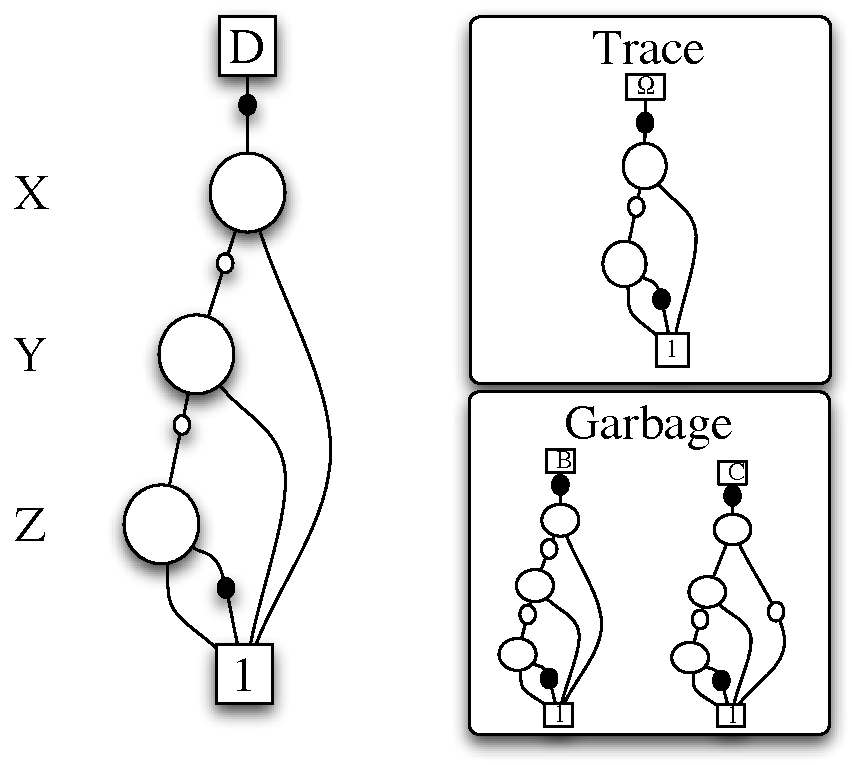
\includegraphics[height=2.5in]{figures/bddtrace04}
  \caption{A BDD for $D$}
  \label{fig:bddtrace04}
\end{figure}

Furthermore, though not shown in this simple example, a similar effect
may occur even without repeated tuples.  If $\Omega$ from prior
iterations of the trace creation loop contained sub-BDDs that would be
useful for future $\Omega's$, they too may be garbage collected and
thus have to be recreated.

The garbage collection process is triggered when system memory is
running low, or when the amount of garbage reaches a threshold set by
the BDD package.  This threshold is generally tuned to balance garbage
collection time and frequency.  If the working set of trace-BDD
creation is less than the threshold for garbage collection, then the
results of many BDD operations will be cached in death row and in the
operation cache.  However, if the working set size of BDD creation is
larger than this threshold, the BDD will free the nodes on death
row. Furthermore, if the working set size of the BDD continues to grow
throughout trace-BDD creation, then garbage collection will occur more
often exacerbating the problem and increasing runtime.

To get an idea of the working set size, we can look at the amount of
garbage produced during trace-BDD construction.
Figure~\ref{fig:164gzipBDDline} shows the number of live BDD nodes and
the total number of BDD nodes present at each sample point in a trace
compression run with automatic garbage collection enabled (a run
without garbage collection quickly exhausts all system memory) vs. the
number of instructions processed in for the $(DIN,DIN)$ BDD for
164.gzip.

\begin{figure}
  \centering
    \includegraphics[width=4.0in]{figures/164gzip_dinvsdin_bdds_linechart}
\caption{BDD Total and Live Nodes}
\label{fig:164gzipBDDline}
\end{figure}

Graphs for trace creation in other SPEC INT benchmarks look similar to
164.gzip.  From the graph we can see that while the number of live
nodes is small, the working set size grows quickly (the spikes in the
graph) until automatic garbage collection reclaims the nodes.  Because
the BDD package must manage this garbage, the package (1) spends most
of its time in garbage collection (see
Figure~\ref{fig:specintbreakdown} for a breakdown of garbage
collection time vs. total trace creation time), and (2) removes the
fraction of nodes that could accelerate BDD creation during garbage
collection.

\begin{figure}
 \subfigure[DIN vs DIN]{
  \includegraphics[width=3.0in]{figures/dindinGCTime}}
  \subfigure[DIN vs SIN]{
  \includegraphics[width=3.0in]{figures/dinsinGCTime}}
  \subfigure[DIN vs RDY]{
  \includegraphics[width=3.0in]{figures/dinrdyGCTime}}
\caption{Break-down of Trace Compression time and Garbage Collection time for select SPEC INT benchmarks.}
\label{fig:specintbreakdown}
\end{figure}

\section{ZDD Compressed Traces}
\label{sec:zddwork}

ZDDs are a variant of BDDs where the \textit{S-deletion} compression
rule is replaced by the use of the \textit{pD-deletion} compression
rule.  In this section we see that ZDDs provide better compression
than BDDs for trace data, and over $9\times$ faster creation times.

\subsection{BDDs vs. ZDDs}

Zero-suppressed BDDs, or ZDDs, replace the \textit{S-deletion} rule with
a the \textit{pD-deletion} rule.  This rule states the following:
\begin{itemize}

\item If the \textit{1} edge from a node \textit{p} leads to a zero
  terminal node and whose \textit{0} edge a child node \textit {q}, then
  \textit{p} is eliminated and all nodes that lead to \textit{p} are
  redirected to \textit{q}.

\end{itemize}

Furthermore, ZDDs do not typically implement the inverting arcs
optimization, i.e., ZDDs have no inverting arcs, only plain $then$ and
$else$ arcs.  To see how this rule change results in a different
decision diagram, consider, once again, the function $f(x,y,z)$ whose
binary decision tree was shown in Figure~\ref{fig:bdtree}a.
Figure~\ref{fig:rozdd} shows the ZDD for this function.

Note, for this function, ZDDs are bad, as most of the values for
$(x,y,z)$ cause the function to evaluate to 1.  However, for sparse
functions (i.e., those with few 1's in the range), such as trace data,
ZDDs are far better.

\subsection{Traces as ZDDs}

To see the advantage of ZDDs for trace creation, let us revisit the
equation $E = \bar{X}\land\bar{Y}\land\bar{Z}$ from
Section~\ref{sec:bddwork}.  The ZDD, with trace-ZDD and garbage, is
shown in Figure~\ref{fig:zddtrace01}.

\begin{figure}
  \centering
  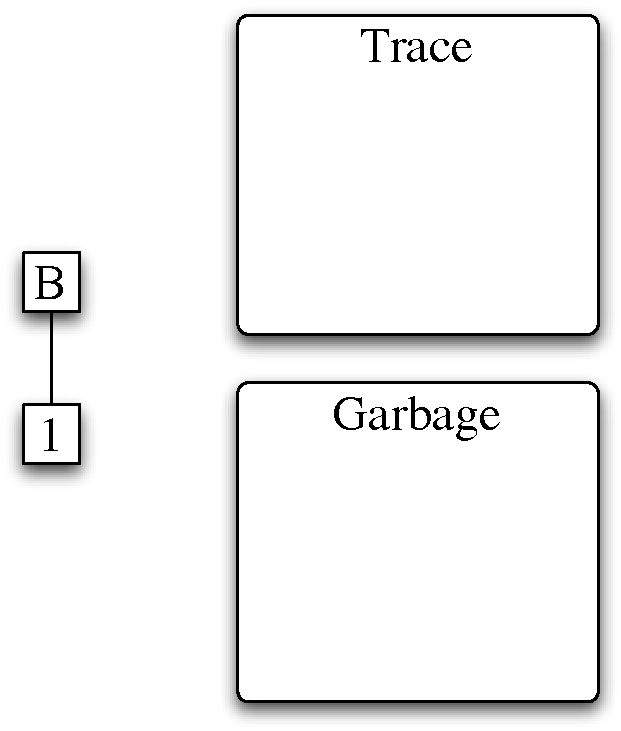
\includegraphics[height=2.5in]{figures/zddtrace01}
  \caption{A ZDD for $\bar{X}\land\bar{Y}\land\bar{Z}$}
  \label{fig:zddtrace01}
\end{figure}

ZDD construction does not apply the \textit{S-deletion} rule, therefore
the resulting graph does contain Boolean \textit{don't - care} values.
However, if a node's $then$ arc terminates at the Boolean false value,
that node is removed.  In the equation $B =
\bar{X}\land\bar{Y}\land\bar{Z}$ all $then$ arcs terminate at 0,
therefore the $X$, $Y$ and $Z$ nodes are removed, leaving a very small
ZDD. We can now construct the trace ZDD for the equation $E' =
X\land\bar{Y}\land\bar{Z}$, as shown in Figure~\ref{fig:zddtrace02}.

\begin{figure}
  \centering
  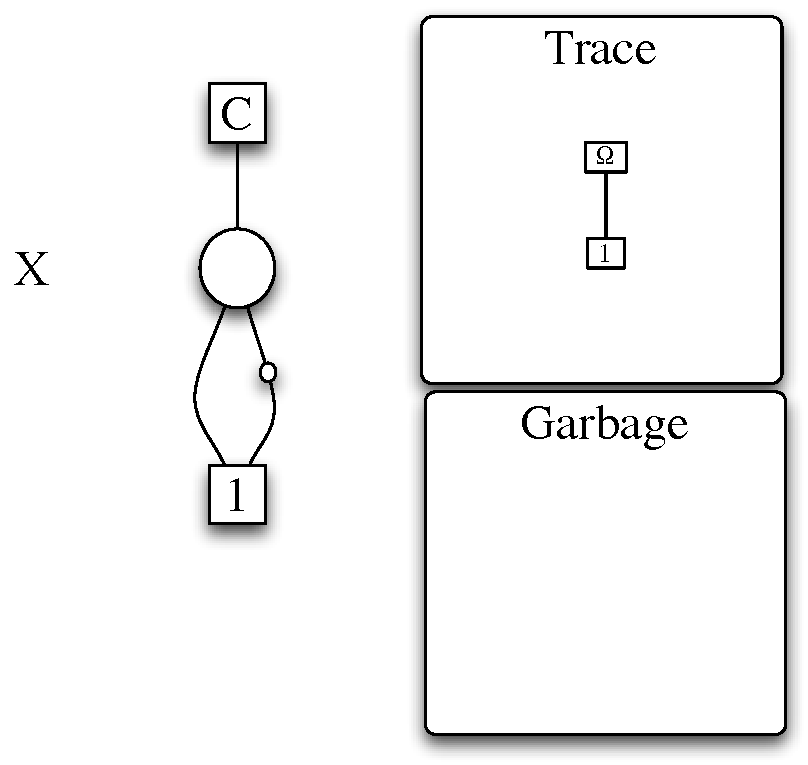
\includegraphics[height=2.5in]{figures/zddtrace02}
  \caption{A ZDD for $X\land\bar{Y}\land\bar{Z}$}
  \label{fig:zddtrace02}
\end{figure}

The ZDD for $E' = X\land\bar{Y}\land\bar{Z}$ now contains a node for
$X$.  Notice $X$ is a boolean \textit{don't-care}, but the BDD
\textit{don't-care} reduction rule has been replaced by the ZDD's
\textit{zero-suppression} rule.  Therefore $X$ is not removed and the $then$
and $else$ arcs point to the same node.

\begin{figure}
  \centering
  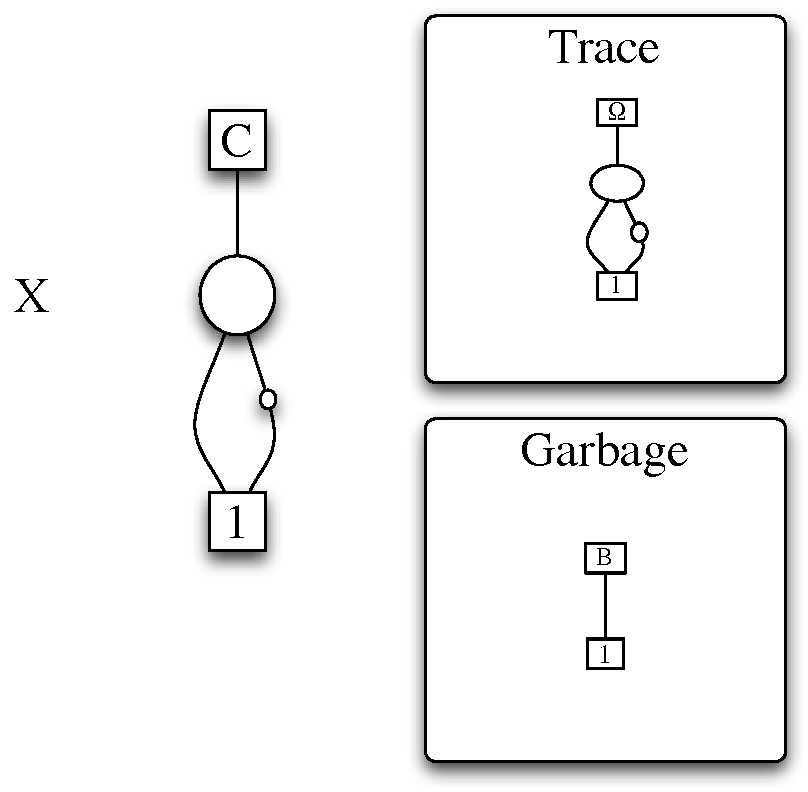
\includegraphics[height=2.5in]{figures/zddtrace03}
  \caption{A ZDD for $B \land C$}
  \label{fig:zddtrace03}
\end{figure}

Figure~\ref{fig:zddtrace03} shows the state of the trace ZDD after the
addition of $E'$.  Notice how little garbage is produced after this
addition.  Now, like the example from Section~\ref{sec:bddwork}, we can
add the function $E''=\bar{X}\land\bar{Y}\land\bar{Z}$, where $E''$ is
equal to $E$.  Like trace-BDD creation, the efficiency of this final
step will depend if garbage collection has occurred between the
creation of $E$, $E'$, and the trace BDD.  However, the ZDD creation
of this trace ZDD produced less garbage than the BDD, therefore it is
less likely to invoke garbage collection.

\begin{figure}
  \centering 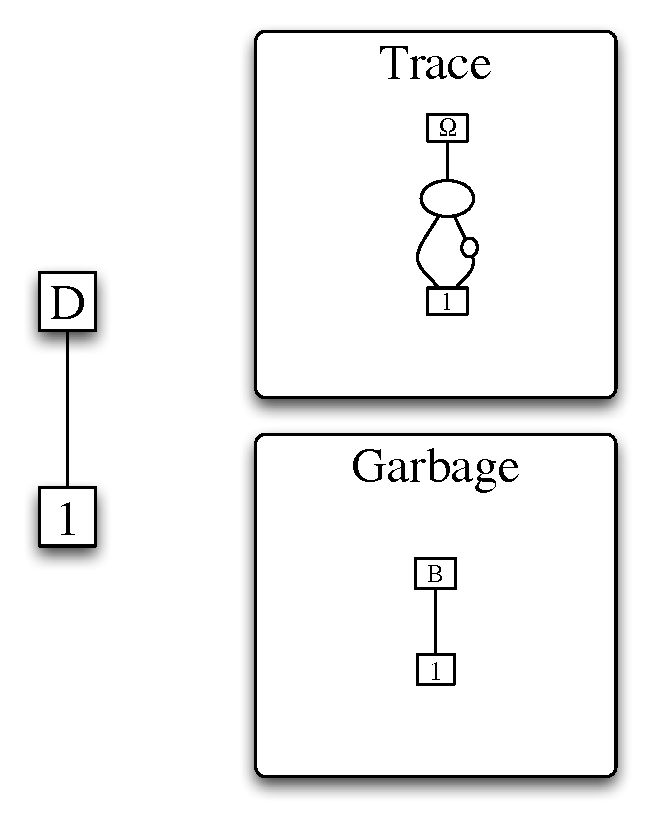
\includegraphics[height=2.5in]{figures/zddtrace04}
  \caption{A ZDD for $B \land C \land D$}
  \label{fig:zddtrace04}
\end{figure}

In both functions $(\bar{X}\land\bar{Y}\land\bar{Z})$ and
$(X\land\bar{Y}\land\bar{Z})$ most $then$ arcs terminate at the false,
or constant zero node. Note that the trace representation method
described in Section~\ref{sec:bddwork} uses nodes that with zero
terminating arcs to represent the binary $0$ in a trace.  Therefore, as
long as the binary representation of such trace data contains many
zeros, and is therefore sparse, ZDDs can achieve good compression.
In fact, ZDDs have been found achieve better compression
levels than BDDs for sets of combinations, as long as the data remains
sparse~\cite{minato:01:STTT}.

Figure~\ref{fig:zddbddSize}, as well as Table~\ref{tab:bddzddsize},
shows that for same set of traces studied in the work in
\cite{price:08:pact} ZDDs achieve approximately 25\% better
compression.  Figure~\ref{fig:zddbddSize} shows the number of nodes
required to represent the BDDs required for various trace analyses and
visualizations.  The data is for 250 million instruction traces from
the SPEC INT 2000 benchmark suite.

\begin{figure}  
  \centering
  \subfigure[DIN vs DIN Node Count]{
  \includegraphics[width=3.2in]{figures/dindinSize}}
  \subfigure[DIN vs SIN Node Count]{
  \includegraphics[width=3.2in]{figures/dinsinSize}}
  \subfigure[DIN vs RDY Node Count]{
  \includegraphics[width=3.2in]{figures/dinrdySize}}
  \caption{DD Node Count}
  \label{fig:zddbddSize}
\end{figure}

\begin{table}
  \small
  \begin{center}
    \subtable[DIN vs RDY]{
    \begin{minipage}{\hsize}
      \renewcommand{\thempfootnote}{\fnsymbol{footnote}}
      \begin{center}
        \begin{tabular}{|r||r|r|r|}
          \hline
          Benchmark & ZDD & BDD\\
          \hline
          164.gzip&14776031&20191795\\
          175.vpr&26758473&39488720\\
          176.gcc&47191021&65452369\\
          181.mcf&13371337&18857151\\
          186.crafty\mpfootnotemark[2]&1426447&1989019\\
          197.parser&20298664&28928181\\
          252.eon&13438978&19243812\\
          253.perlbmk&15447265&22507110\\
          254.gap&18167754&24067457\\
          255.vortex\mpfootnotemark[2]&193184&260701\\
          256.bzip2\mpfootnotemark[2]&101730&138353\\
          300.twolf&26470707&36674682\\
          \hline
        \end{tabular}
      \end{center}
    \end{minipage}
    }
    \subtable[DIN vs SIN]{
    \begin{minipage}{\hsize}
      \renewcommand{\thempfootnote}{\fnsymbol{footnote}}
      \begin{center}
        \begin{tabular}{|r||r|r|r|}
          \hline
          Benchmark & ZDD & BDD\\
          \hline
          164.gzip&2395329&2954172\\
          175.vpr&6220387&8094630\\
          176.gcc&16477762&22851246\\
          181.mcf&4166872&5302426\\
          186.crafty\mpfootnotemark[2]&664726&944032\\
          197.parser&4346929&5561810\\
          252.eon&5758390&8175031\\
          253.perlbmk&2728992&3490785\\
          254.gap&3563179&4998176\\
          255.vortex\mpfootnotemark[2]&140930&212049\\
          256.bzip2\mpfootnotemark[2]&61088&89025\\
          300.twolf&5912991&7515602\\
          \hline
        \end{tabular}
      \end{center}
    \end{minipage}
    }
    \subtable[DIN vs DIN]{
    \begin{minipage}{\hsize}
      \renewcommand{\thempfootnote}{\fnsymbol{footnote}}
      \begin{center}
        \begin{tabular}{|r||r|r|r|}
          \hline
          Benchmark & ZDD & BDD\\
          \hline
          164.gzip&22014614&28903561\\
          175.vpr&27382836&41901557\\
          176.gcc&51666471&76472039\\
          181.mcf&5669206&8109996\\
          186.crafty\mpfootnotemark[2]&1438765&2081447\\
          197.parser&25075154&35929906\\
          252.eon&7925540&12075596\\
          253.perlbmk&10525806&15667727\\
          254.gap&13014623&17960509\\
          255.vortex\mpfootnotemark[2]&226433&312175\\
          256.bzip2\mpfootnotemark[2]&113627&157461\\
          300.twolf&21568405&34202383\\
          \hline
        \end{tabular}
      \end{center}
    \footnotetext[1]{Full benchmark trace, benchmark ran to completion.}
    \end{minipage}
    }
    \caption{BDD vs ZDD Node Count}
    \label{tab:bddzddsize}
  \end{center}
\end{table}

\subsection{ZDD Variable Order, Visualization, and Analysis}

It is important to note that ZDD and BDD size can vary significantly
depending on the choice variable order.  Furthermore, the choice of
the best variable order for a ZDD may not be the same as the best
order for the equivalent BDD.  This can be problematic, as discussed
in Section~\ref{sec:visual}, as certain visualization algorithms
depend on the variable order in the ZDD.  Fortunately, Lhot\'{a}k
\textit{et. al.} found that in many cases the best BDD variable order
is also the best ZDD variable order~\cite{lhotak:08:lcpc}.  Lhot\'{a}k
\textit{et. al.} also show that it is trivial to convert any BDD-based
program analysis into a ZDD-based analysis.  Applying Lhot\'{a}k
\textit{et. al.}'s insight and the concept of BDD-encoded dynamic
traces~\cite{price:06:cal}, all the standard analyses can also be
applied to ZDD compressed traces.  The one non-trivial algorithm is
the trace visualization algorithm used by the ParaMeter
tool~\cite{price:08:pact}.  However, Section~\ref{sec:visual} shows
how to adapt this algorithm used for ZDDs.

\subsection{ZDD Compression Time}

BDD compression time may increase as node count
decreases~\cite{price:08:msthesis}. However, the ZDD unique
table growth in Figure~\ref{fig:164gzipZDDline} (compared to
Figure~\ref{fig:164gzipBDDline}) shows that far less garbage is
produced during trace-ZDD creation.
\begin{figure}
  \centering
    \includegraphics[width=4.5in]{figures/164gzip_dinvsdin_zdds_linechart}
\caption{ZDD Total and Live Nodes}
\label{fig:164gzipZDDline}
\end{figure}
Because there is far less garbage produced, the ZDD-based trace
compressor spends far less time collecting garbage.
Figure~\ref{fig:zddbddGC} compares the amount of time required for
garbage collection for ZDD and BDD encoded traces for the set of trace
data used by ParaMeter~\cite{price:08:pact}. These figures are also
presented in Table~\ref{tab:bddzddgctime}. Notice that the ZDD-based
code spends far less time collecting garbage.

\begin{figure}
  \centering
  \subfigure[DIN vs DIN Garbage Collection Time]{
  \includegraphics[width=4.0in]{figures/dindinGC}}
  \subfigure[DIN vs SIN Garbage Collection Time]{
  \includegraphics[width=4.0in]{figures/dinsinGC}}
  \subfigure[DIN vs RDY Garbage Collection Time]{
  \includegraphics[width=4.0in]{figures/dinrdyGC}}
  \caption{DD Garbage Collection Time}
  \label{fig:zddbddGC}
\end{figure}

\begin{table}
  \small
  \begin{center}
    \subtable[DIN vs RDY]{
    \begin{minipage}{\hsize}
      \renewcommand{\thempfootnote}{\fnsymbol{footnote}}
      \begin{center}
        \begin{tabular}{|r||r|r|r|}
          \hline
          Benchmark & ZDD & BDD\\
          \hline
          164.gzip&6149&34744\\
          175.vpr&9395&60352\\
          176.gcc&18260&86119\\
          181.mcf&4970&33083\\
          186.crafty\mpfootnotemark[2]&69&505\\
          197.parser&7881&51172\\
          252.eon&6478&46865\\
          253.perlbmk&6417&41291\\
          254.gap&5232&34420\\
          255.vortex\mpfootnotemark[2]&1&10\\
          256.bzip2\mpfootnotemark[2]&14&97\\
          300.twolf&8511&51914\\
          \hline
        \end{tabular}
      \end{center}
    \end{minipage}
    }
    \subtable[DIN vs SIN]{
    \begin{minipage}{\hsize}
      \renewcommand{\thempfootnote}{\fnsymbol{footnote}}
      \begin{center}
        \begin{tabular}{|r||r|r|r|}
          \hline
          Benchmark & ZDD & BDD\\
          \hline
          164.gzip&20522&92132\\
          175.vpr&18718&114093\\
          176.gcc&47518&201188\\
          181.mcf&7704&63987\\
          186.crafty\mpfootnotemark[2]&143&1196\\
          197.parser&20720&114329\\
          252.eon&10218&82897\\
          253.perlbmk&9549&68938\\
          254.gap&11944&75353\\
          255.vortex\mpfootnotemark[2]&3&19\\
          256.bzip2\mpfootnotemark[2]&38&216\\
          300.twolf&13663&100911\\
          \hline
        \end{tabular}
      \end{center}
    \end{minipage}
    }
    \subtable[DIN vs DIN]{
    \begin{minipage}{\hsize}
      \renewcommand{\thempfootnote}{\fnsymbol{footnote}}
      \begin{center}
        \begin{tabular}{|r||r|r|r|}
          \hline
          Benchmark & ZDD & BDD\\
          \hline
          164.gzip&1964&12410\\
          175.vpr&3879&30428\\
          176.gcc&7184&44513\\
          181.mcf&3447&26368\\
          186.crafty\mpfootnotemark[2]&69&262\\
          197.parser&3042&28573\\
          252.eon&4001&32793\\
          253.perlbmk&2298&21147\\
          254.gap&2547&24172\\
          255.vortex\mpfootnotemark[2]&2&9\\
          256.bzip2\mpfootnotemark[2]&18&90\\
          300.twolf&3315&31596\\
          \hline
        \end{tabular}
      \end{center}
    \footnotetext[1]{Full benchmark trace, benchmark ran to completion.}
    \end{minipage}
    }
    \caption{BDD vs ZDD Garbage Collection Time (Seconds)}
    \label{tab:bddzddgctime}
  \end{center}
\end{table}

Now that we know that ZDDs have a small working set size and that the
amount of garbage produced stays almost flat during trace-ZDD
creation, it is possible to further accelerate ZDD trace creation by
adjusting the size of the unique table so that it will contain the
working set of the trace-ZDD.  

In Figure ~\ref{fig:zddbddtime}, and Table
~\ref{tab:bddzddcreationtime}, we can see the time, in seconds,
required to encode 250 million trace instructions into a ZDD compared
to the time required by BDDs.  In this figure, the size of the unique
table was manually increased to be initially 100x the normal size for
both BDD and ZDD based creation. Note that because BDDs generate so
much garbage, their working set size is much larger than available
RAM, meaning that they gain little benefit from the 100x increase in
table size.  ZDDs on the other hand are much faster because the larger
unique table can fit almost the entire working set of useful BDD
nodes, and garbage does not cause these nodes to be reaped from death
row and the operation cache.

\begin{figure}
  \centering
  \subfigure[DIN vs DIN Creation Time]{
  \includegraphics[width=4.0in]{figures/dindinTime}}
  \subfigure[DIN vs SIN Creation Time]{
  \includegraphics[width=4.0in]{figures/dinsinTime}}
  \subfigure[DIN vs RDY Creation Time]{
  \includegraphics[width=4.0in]{figures/dinrdyTime}}
  \caption{DD Creation Time}
  \label{fig:zddbddtime}
\end{figure}

\begin{table}
  \small
  \begin{center}
    \subtable[DIN vs RDY]{
    \begin{minipage}{\hsize}
      \renewcommand{\thempfootnote}{\fnsymbol{footnote}}
      \begin{center}
        \begin{tabular}{|r||r|r|r|}
          \hline
          Benchmark & ZDD & BDD\\
          \hline
          164.gzip&11487&61046\\
          175.vpr&15699&87107\\
          176.gcc&24612&116137\\
          181.mcf&9995&57038\\
          186.crafty\mpfootnotemark[2]&219&1495\\
          197.parser&13392&79809\\
          252.eon&11817&73301\\
          253.perlbmk&11773&64993\\
          254.gap&10145&59557\\
          255.vortex\mpfootnotemark[2]&5&25\\
          256.bzip2\mpfootnotemark[2]&50&469\\
          300.twolf&14125&77106\\
          \hline
        \end{tabular}
      \end{center}
    \end{minipage}
    }
    \subtable[DIN vs SIN]{
    \begin{minipage}{\hsize}
      \renewcommand{\thempfootnote}{\fnsymbol{footnote}}
      \begin{center}
        \begin{tabular}{|r||r|r|r|}
          \hline
          Benchmark & ZDD & BDD\\
          \hline
          164.gzip&6100&37454\\
          175.vpr&10532&55314\\
          176.gcc&14015&76713\\
          181.mcf&8974&48328\\
          186.crafty\mpfootnotemark[2]&268&1385\\
          197.parser&9214&52987\\
          252.eon&10503&56826\\
          253.perlbmk&7779&44185\\
          254.gap&8013&48764\\
          255.vortex\mpfootnotemark[2]&7&25\\
          256.bzip2\mpfootnotemark[2]&71&526\\
          300.twolf&9558&56593\\
          \hline
        \end{tabular}
      \end{center}
    \end{minipage}
    }
    \subtable[DIN vs DIN]{
    \begin{minipage}{\hsize}
      \renewcommand{\thempfootnote}{\fnsymbol{footnote}}
      \begin{center}
        \begin{tabular}{|r||r|r|r|}
          \hline
          Benchmark & ZDD & BDD\\
          \hline
          164.gzip&33581&156663\\
          175.vpr&34234&178788\\
          176.gcc&64607&276295\\
          181.mcf&21517&121063\\
          186.crafty\mpfootnotemark[2]&521&3711\\
          197.parser&35717&178564\\
          252.eon&24280&147433\\
          253.perlbmk&21072&125391\\
          254.gap&25234&143287\\
          255.vortex\mpfootnotemark[2]&10&61\\
          256.bzip2\mpfootnotemark[2]&132&1099\\
          300.twolf&27167&162679\\
          \hline
        \end{tabular}
      \end{center}
    \footnotetext[1]{Full benchmark trace, benchmark ran to completion.}
    \end{minipage}
    }
    \caption{BDD vs ZDD Creation Time (Seconds)}
    \label{tab:bddzddcreationtime}
  \end{center}
\end{table}
\section{ZDD Dependence Visualization}
\label{sec:visual}

Section~\ref{sec:zddwork} described how to trivially extend BDD-based
trace analysis to ZDDs by leveraging prior work.  The visualization
scheme used by ParaMeter allows interactive identification, analysis,
and extraction of parallelism based on BDD-compressed
traces~\cite{price:08:pact}.  However, this visualization algorithm is
specific to BDDs.  Given the promise of this approach, we show that it
is possible to apply the same with techniques on ZDDs with only slight
modifications.

\subsection{DINxRDY Visualization}

The ParaMeter tool, used throughout this thesis, creates a
visualization based on the DINxRDY plot, originally introduced by
Postiff \textit{et. al.}~\cite{postiff:98:um}.  An example DINxRDY plot is shown
in Figure \ref{fig:sampledinvrdy}.

DINxRDY plots can show potential regions of parallelism as follows (as
first described by Iyer \textit{et. al.}~\cite{iyer:05:epic}).  Lines
in a DINxRDY plot that run from the lower-left to upper right form
dependence chains of relatively nearby
instructions~\cite{iyer:05:epic}.  Iyer \textit{et. al.} found that
diagonal lines with overlapping x-extents could potentially represent
regions of code that have the potential to be parallelized (circled in
the Figure~\ref{fig:sampledinvrdy}).  DINxRDY plots can be used to
find and extract parallelism by locating a region in a DINxRDY plot
with overlapping x-extents in the 175.vpr
benchmark~\cite{price:08:pact}.  Using classic program analyses
applied to traces, this example extracted both data and pipeline
parallelism from the benchmark.

\subsection{Extended Visualization Algorithm}

It is possible to generate visualizations from trace-BDDs in
milliseconds by treating the BDD structure like a
quad-tree~\cite{price:08:pact}.  To understand this algorithm,
consider Figures~\ref{fig:quadtree} and \ref{fig:samplequadtreeds}.

In graphics, a quad-tree decomposes two-dimensional image data into
hierarchical regions. Figure~\ref{fig:samplequadtreeds} shows a quad
tree for the DINxRDY graph shown in Figure~\ref{fig:quadtree}.  The
region outlined on Figure~\ref{fig:quadtree} represents its
decomposition, where node N$i$ corresponds to the region $i$ in the
figure.

\begin{figure}
\begin{center}
\tiny
\begin{picture}(0,0)
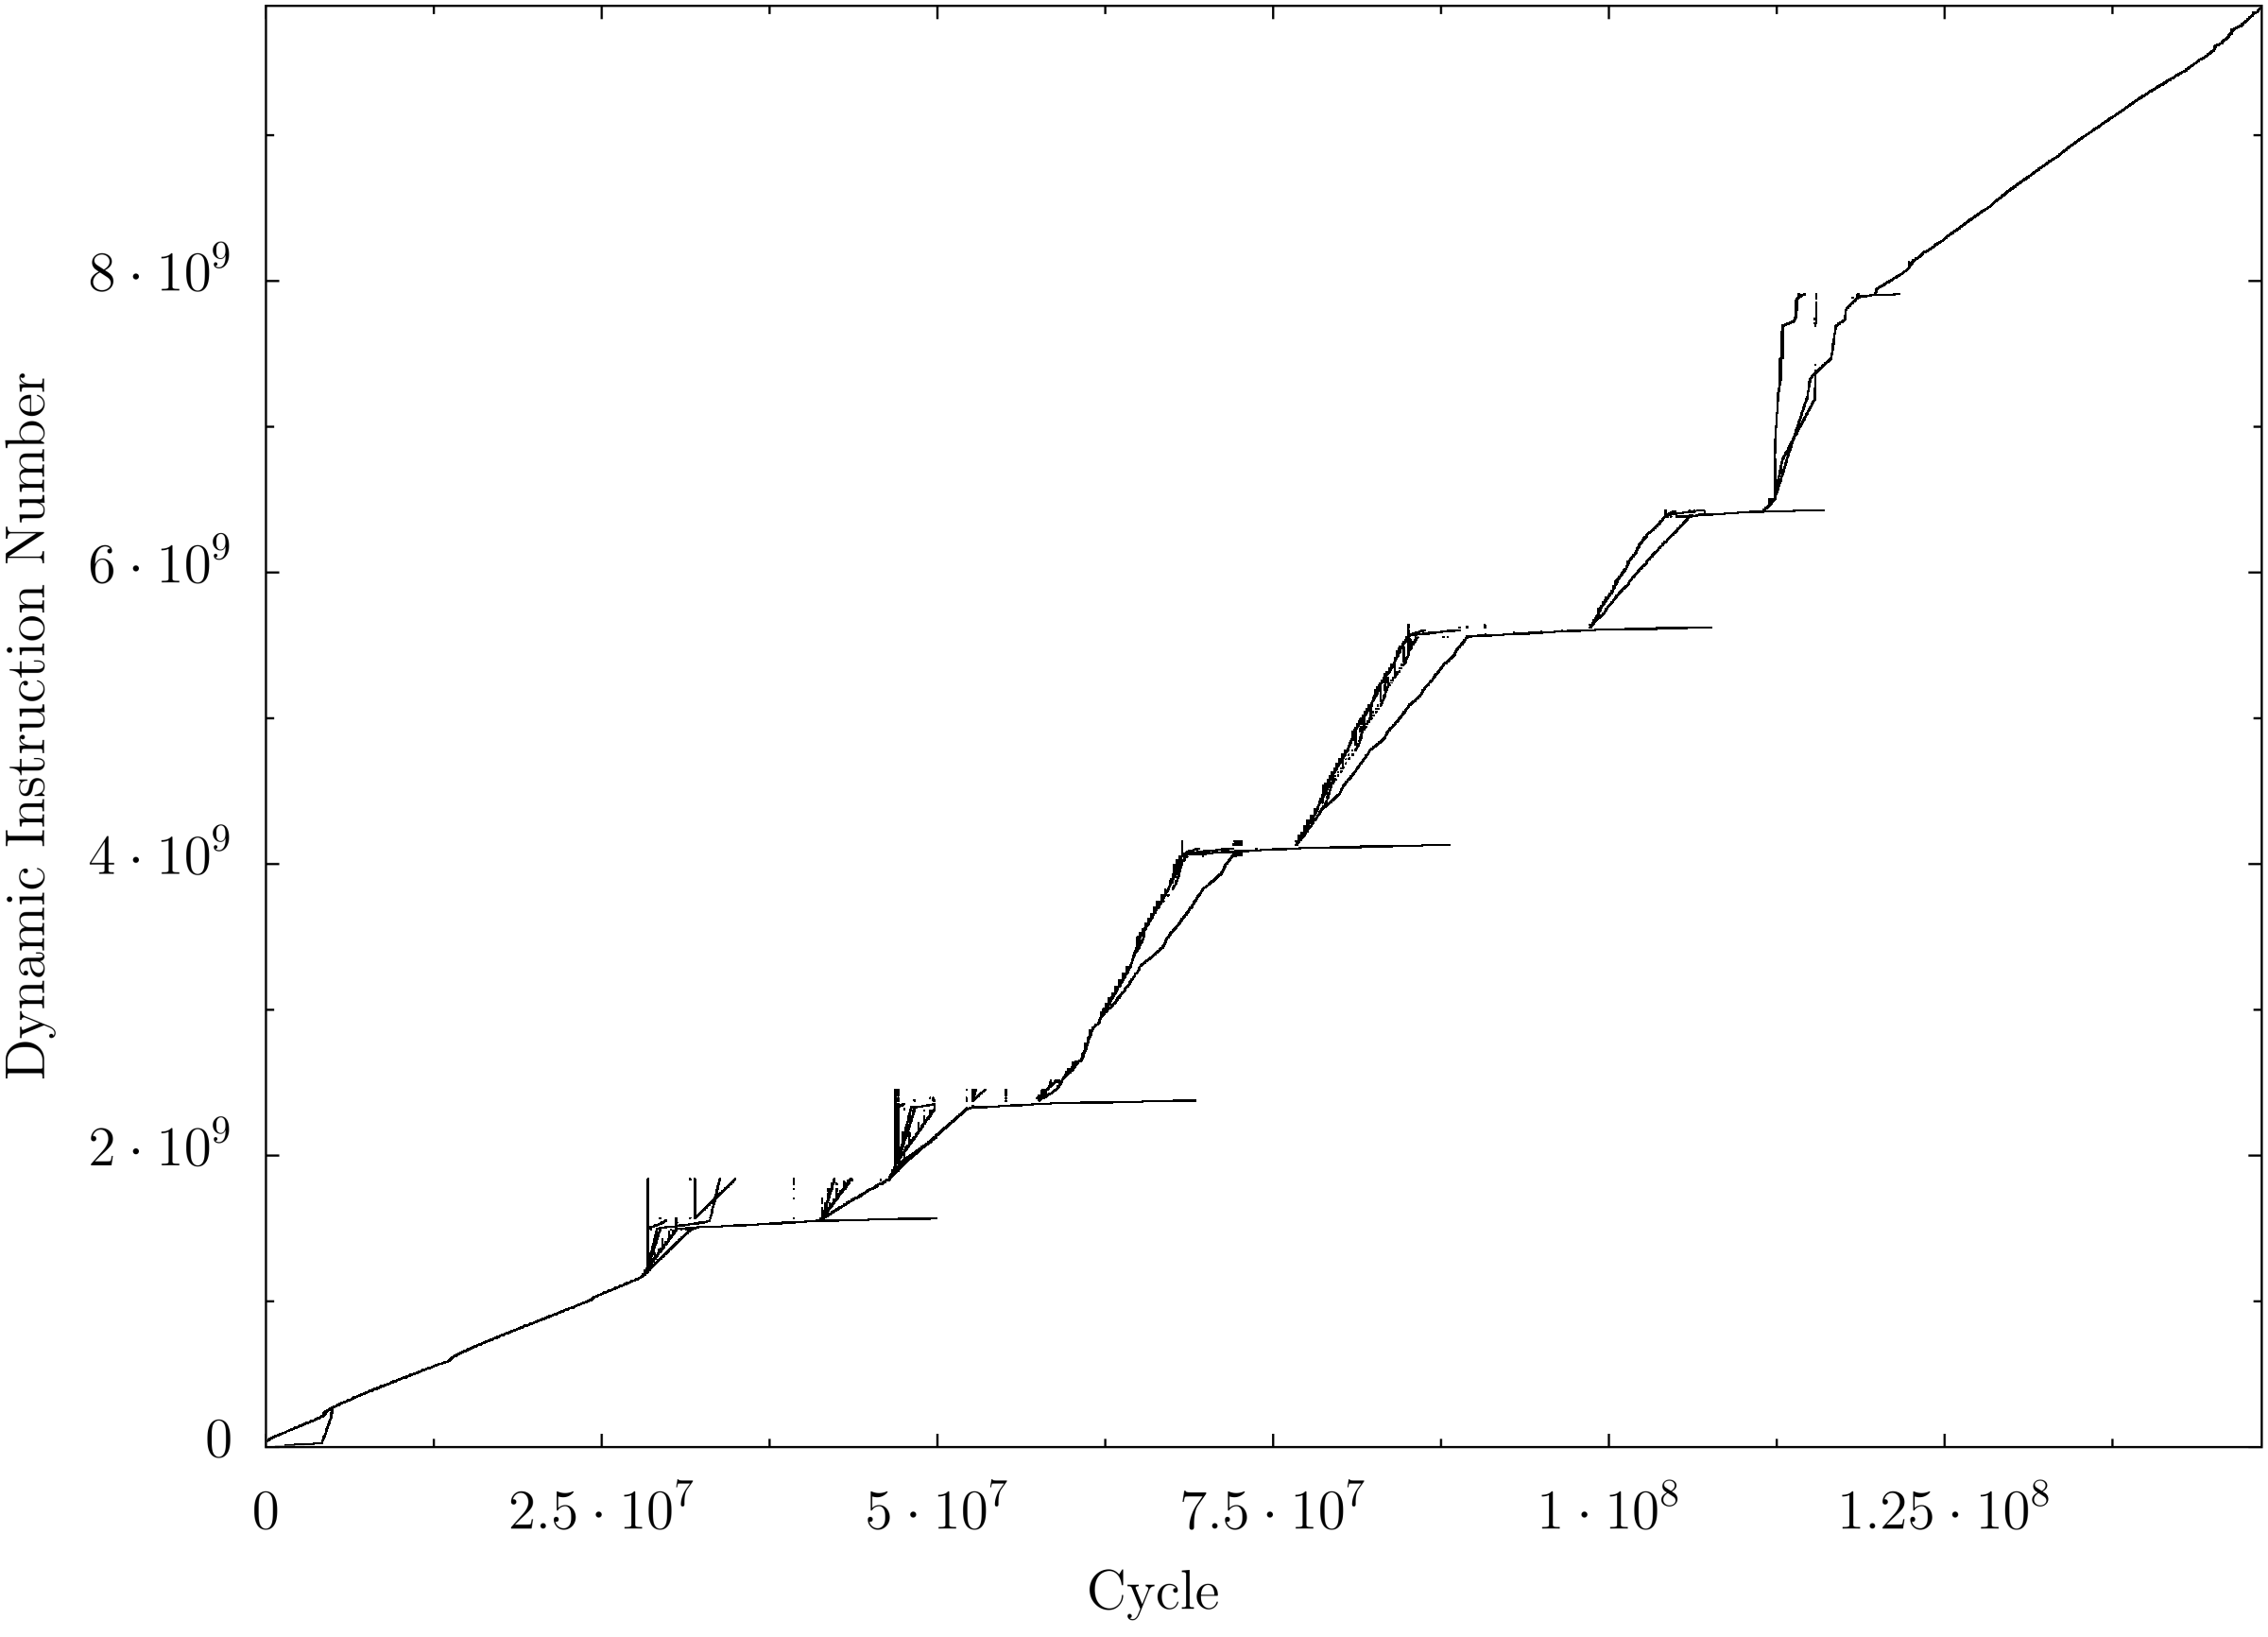
\includegraphics[width=3in]{figures/ia64_254_gap_gcc_inf_bw_din_crop2}
\end{picture}
\begin{picture}(225,155)
\put(24,19) {\framebox(68,68){}}
\put(24,87) {\framebox(68,68){Empty (1)}}
\put(92,19) {\framebox(68,68){}}
\put(92,87) {\framebox(68,68){}}

\put(24,19) {\framebox(34,34){(3.3)}}
\put(24,53) {\framebox(34,34){Empty (3.1)}}
\put(58,19) {\framebox(34,34){(3.4)}}
\put(58,53) {\framebox(34,34){Empty (3.2)}}

\put(92,19) {\framebox(34,34){(4.3)}}
\put(92,53) {\framebox(34,34){(4.1)}}
\put(126,19) {\framebox(34,34){Empty (4.4)}}
\put(126,53) {\framebox(34,34){(4.2)}}

\put(92,87) {\framebox(34,34){Empty (2.3)}}
\put(92,121) {\framebox(34,34){Empty (2.1)}}
\put(126,87) {\framebox(34,34){(2.4)}}
\put(126,121) {\framebox(34,34){Empty (2.2)}}
\end{picture}
\end{center}
\caption{Sample partial quad-tree regions superimposed a DINxRDY plot
of SPEC INT 2000 benchmark 254.gap. (Not to scale)}
\label{fig:quadtree}
\end{figure}

\begin{figure}
\begin{center}
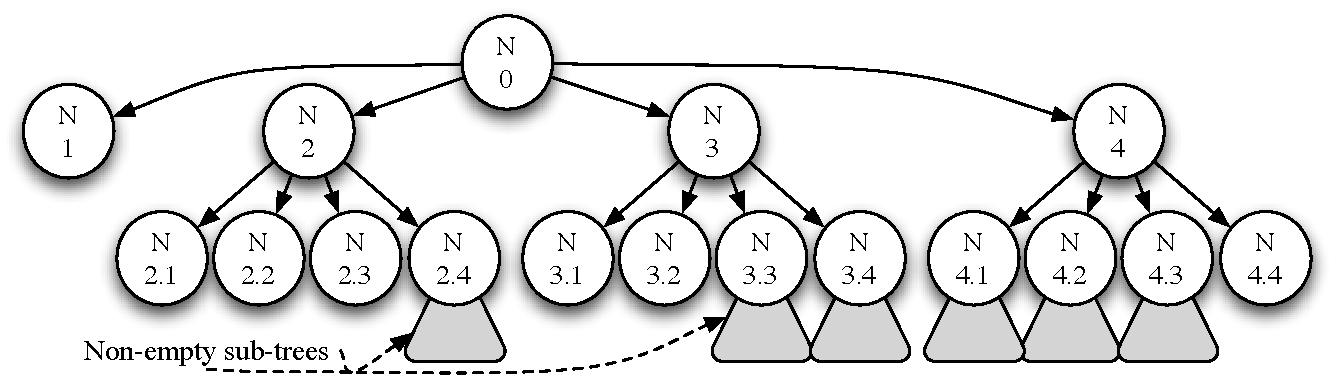
\includegraphics[width=4.5in]{figures/samplequadtreeds}
\end{center}
\caption{Sample partial quad-tree for regions in Figure~\ref{fig:quadtree}}
\label{fig:samplequadtreeds}
\end{figure}

The visualization algorithm used by ParaMeter is straightforward.
Under the variable ordering used in this work, if a BDD is traversed
like a tree, then the even levels correspond to bisecting each region
horizontally, and the odd levels correspond to bisecting each region
vertically.  Thus traversing two levels of the BDD corresponds to
traversing a single level of the corresponding quad tree.  However,
since BDDs use the \textit{S-deletion} rule to eliminate nodes, this
algorithm must account for eliminated nodes.  Since ZDDs use a
\textit{pD-deletion} rule, the algorithm for BDDs applies to
ZDDs with only a change to how missing levels in the ZDD traversal are
handled and what to do when the terminal state is reached.

Recall that the \textit{S-deletion} rule removes nodes from a BDD when
both the 1 and 0 outgoing branches lead to the same child node.  The
quad-tree graphing algorithm must detect removed BDD nodes before
graphing the extracted data.  For example, consider the indicator
function
$(\bar{X}\land\bar{Y}\land\bar{Z})\lor(X\land\bar{Y}\land\bar{Z})$.
This function represents the set of two numbers $\{000, 100\}$.  In the
BDD for this function, shown in Figure~\ref{fig:bddtrace03} the node
for $X$ was removed because it is a boolean \textit{don't care}.
Thus, the algorithm used by ParaMeter has to virtually traverse the
graph shown in Figure~\ref{fig:bddGraph} instead.  To do this,
ParaMeter detects that a variable was skipped during traversal and
then orchestrates its traversal to virtually traverse outgoing arcs
from the removed node, which is shown in grey.  If a traversal through
the BDD reveals many removed nodes, the number of new arcs grows
exponentially in the number of \textit{don't care} values, however,
ParaMeter implements a number of optimizations to terminate traversals
early, limiting the exponential explosion.

To adapt this algorithm to ZDDs we must understand how to deal with
missing nodes.  In practice, the final algorithm is simpler than that for BDDs
because the \textit{pD-reduction} rule does not have to be undone like
the \textit{S-deletion} rule.

\begin{figure}
\begin{center}
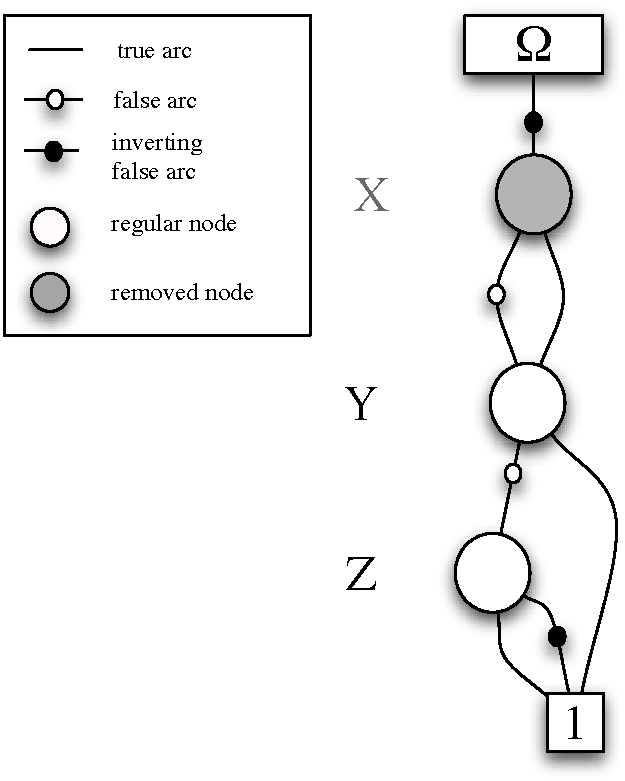
\includegraphics[height=2.5in]{figures/bddgraphEx1}
\end{center}
\caption{Graph BDD With Missing Node}
\label{fig:bddGraph}
\end{figure}

\begin{figure}
\begin{center}
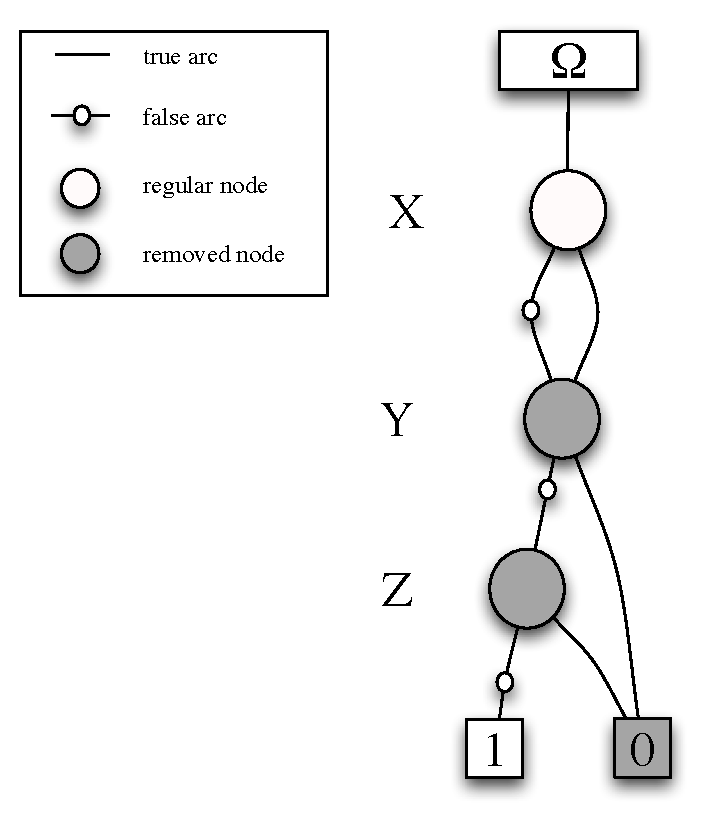
\includegraphics[height=2.5in]{figures/zddgraphEx1}
\end{center}
\caption{Graph ZDD With Missing Nodes}
\label{fig:zddGraph}
\end{figure}

In Figure~\ref{fig:zddGraph} we can see the ZDD for the function
$(\bar{X}\land\bar{Y}\land\bar{Z})\lor(X\land\bar{Y}\land\bar{Z})$
with removed nodes also highlighted in grey.  Notice that, as per the
pD-deletion rule, all of the removed nodes have \textit{then} branches
leading to the $0$ terminal case. Therefore, any time the graphing
algorithm detects a removed node, it knows that there is no need to
traverse the half of the region where the variable of the missing node
is true, and thus needs to do no work.  For the half where the
variable is false, the algorithm virtually traverses the else-edge of
the missing node, just as the BDD-based algorithm traversed both the
then and the else edges.
\begin{figure}
 \begin{center}
  \includegraphics[width=4.5in]{figures/visualizationTime}  
 \end{center}
 \caption{ZDD and BDD Visualization Time for SPEC INT 2000 benchmarks}
 \label{fig:visualTime}
\end{figure}
Accordingly, Figure~\ref{fig:visualTime} shows ZDD rendering is
slightly faster than BDDs.  Data is from a 2.8 GHz Intel
Core i7 with 12~GB of RAM running Linux.
%%%%%%%%%%%%%%%%%%%%%%%%%%%%%%%%%%%%%%%%%%%%%%%%%%%%%%%%%%%%%%%%%%%%%%%%%%%%%
\chapter{ZDD-based Dynamic Trace Slicing and Chopping}
\label{chap:zddchop}
%%%%%%%%%%%%%%%%%%%%%%%%%%%%%%%%%%%%%%%%%%%%%%%%%%%%%%%%%%%%%%%%%%%%%%%%%%%%%

The pseudo code in Figure~\ref{fig:bddslice} shows how to compute the
reverse slice of an instruction with a BDD-encoded DIN
$d$~\cite{price:06:cal}.  In this pseudo-code, $e$ is given as the
indicator function for the set of edges in the data dependence graph,
$I_d$ is given as the indicator function for the instruction with DIN
$d$, and $s$ is the indicator function for the reverse slice that is
computed~\cite{price:06:cal}.  The variables in indicator function
$I_d$ are in the vector $\mathbf{d^1}$, the variables in $s$ are also
in vector $\mathbf{d^1}$, and the variables in $e$ are
$(\mathbf{d^1},\mathbf{d^2})$.  The function $\mathrm{rename}$ takes a
function $s$ and renames the variables from set $\mathbf{d^2}$ to the
corresponding variables in set $\mathbf{d^1}$.

\begin{figure}
\begin{center}
\begin{minipage}{1.5in}
\begin{tabbing}
\hspace{1em}\=\hspace{1em}\=\hspace{1em}\=\hspace{1em}\=\\
\textbf{function} reverse\_slice\_bdd($e$,$I_d$)\\
\>$s := I_d$\\
\>$s = \mathrm{rename}(\mathbf{d^1},\mathbf{d^2},s)$\\
\>$e' := e \land s$\\
\>$s := \exists \mathbf{d^2}.e'$\\
\>\textbf{return} $s$
\end{tabbing}
\end{minipage}
\end{center}
\caption{Computing a Reverse Slice using BDDs.~\cite{price:06:cal}}
\label{fig:bddslice}
\end{figure}

Slicing depends on the use of existential quantification to remove
variables. In the pseudo code in Figure~\ref{fig:bddslice} the
$\exists$ function uses existential quantification to remove the
variables $e'$ from the dynamic instructions in $\mathbf{d^2}$.  When
using BDDs, variables that are removed are interpreted as boolean
\textit{don't care} values.  However, variables that are removed from
a ZDD are interpreted as zero values.

Thus, in order to perform operations that depend on \textit{don't
  care} values, an additional step is taken to insert \textit{don't
  care} values.  The slicing algorithm shown in
Figure~\ref{fig:zddITEslice} uses the function $\mathrm{yDC}(d)$ to
insert \textit{don't care} values in the $y$ variable positions.  This
function, given the variable positions for the tuple $(x,y)$ and an
identity function $d$, will return the ZDD dot
product\cite{mishchenko:01:sc} of the function $d$ and the universal
set of bits for tuple variable $y$.  A similar function,
$\mathrm{xDC(s)}$, is used for forward slicing.

Let $C$ and $D$ be two trace encoded ZDDs.  The unate product of two
trace ZDDs is defined as $0 \ if \ \exists x(x \in C \cup D \ and \ x' \in
C \cup D)$, otherwise $C \cup D$~\cite{hachtel:00:kap}.

\begin{figure}
\begin{center}
\begin{minipage}{1.5in}
\begin{tabbing}
\hspace{1em}\=\hspace{1em}\=\hspace{1em}\=\hspace{1em}\=\\
\textbf{function} reverse\_slice\_zdd($e$,$I_d$)\\
\>$s := I_d$\\
\>$s = \mathrm{rename}(\mathbf{d^1},\mathbf{d^2},s)$\\
\>$s = \mathrm{yDC}(s)$\\
\>$e' := e * s$\\
\>$s := \exists \mathbf{d^2}.e'$\\
\>\textbf{return} $s$
\end{tabbing}
\end{minipage}
\end{center}
\caption{Computing a Reverse Slice using ZDD Unate Product.}
\label{fig:zddUPslice}
\end{figure}

Note that the If-Then-Else (ITE) operation can be used to create a
logic conjunction.  For example, $C \wedge D$ is logically equivalent
to $if(C) \ then(D) \ else \ 0$.  If $x$ is a literal, for $\exists x
\in C \wedge \exists x \in D | $.  If $x \not \in C \vee x \not \in
D|0$.  Missing variables are treated like $0$, and not like a Boolean
\textit{don't care}.  Thus, the $ITE$, using bit vectors encoded as
ZDDs, captures the logic $and$ behavior used in slicing.

\begin{figure}
\begin{center}
\begin{minipage}{1.5in}
\begin{tabbing}
\hspace{1em}\=\hspace{1em}\=\hspace{1em}\=\hspace{1em}\=\\
\textbf{function} ITE\_slice\_zdd($e$,$I_d$)\\
\>$I_d' = \mathrm{rename}(\mathbf{d^1},\mathbf{d^2},I_d')$\\
\>$e' = \mathrm{yDC}(e)$\\
\>$s := ite(I_d',e',zero)$\\
\>$s' := \exists \mathbf{d^2}.s$\\
\>\textbf{return} $s'$
\end{tabbing}
\end{minipage}
\end{center}
\caption{Computing an Reverse Slice using ZDD ITE.}
\label{fig:zddITEslice}
\end{figure}

When ZDD functions are unate, the ZDD intersection operation
does not take the place of the logic conjunction. 

\begin{figure}
\begin{center}
\begin{minipage}{1.5in}
\begin{tabbing}
\hspace{1em}\=\hspace{1em}\=\hspace{1em}\=\hspace{1em}\=\\
\textbf{function} reverse\_slice\_zdd($e$,$I_d$)\\
\>$s := I_d$\\
\>$s = \mathrm{rename}(\mathbf{d^1},\mathbf{d^2},s)$\\
\>$s = \mathrm{yDC}(s)$\\
\>$e' := e \cap s$\\
\>$s := \exists \mathbf{d^2}.e'$\\
\>\textbf{return} $s$
\end{tabbing}
\end{minipage}
\end{center}
\caption{Computing an Reverse Slice using ZDD Intersection.}
\label{fig:zddIntersectSlice}
\end{figure}

\section{ZDD Slice Performance}
\label{sec:zddsliceperf}

It is possible for a DDG slice to iterate billions of times before
reaching a fixed point.  Therefore, even a small decrease in slice
time can be multiplied into substantial overall increase in
performance.  This section compares the slicing performance for the
\textit{ITE} and the \textit{Intersect} techniques.  The
\textit{product} slicing algorithm fails to complete in a reasonable
amount of time (one week) for these slicing tests.  In fact, a
\textit{product} based slice fails for DDGs with only 1 million nodes.

\subsection {Experimental Setup}

Each ZDD slicing technique was tested using a 2.6 GHz Xeon server with
32 GB of RAM.  Each slice starts from an initial set of 10, 100, 1000,
or 10000 randomly selected instructions from a set of 1 billion
instructions. Each slicing operation was repeated six to ten times;
the final results in Figure~\ref{fig:slicing} shows the arithmetic
mean.

\begin{figure}
  \centering
  \subfigure[10 Initial Instructions]{
    \includegraphics[width=4in]{figures/slice10}
    \label{fig:slice10}
  }
  \subfigure[100 Initial Instructions]{
    \includegraphics[width=4in]{figures/slice100}
    \label{fig:slice100}
  }
  \subfigure[1000 Initial Instructions]{
    \includegraphics[width=4in]{figures/slice1000}
    \label{fig:slice1000}
  }
  \subfigure[10000 Initial Instructions]{
    \includegraphics[width=4in]{figures/slice10000}
    \label{fig:slice10000}
  }
  \label{fig:slicing}
  \caption[Slicing times]{Slicing Times}
\end{figure}

These results show that for most operations ZDD slicing via
intersection performs better than the ITE method.  Therefore, other
analyses in this thesis that depend on a program slice will use
intersection.  The intersection technique still requires more steps
than the comparable BDD slice.  Analyses in this thesis that use
slicing would likely benefit from a unification of operations used for
ZDD slicing, similar to the work by Lhotak \textit{et. al.} with relational
operations used for points-to analysis~\cite{lhotak:08:lcpc}.

%%%%%%%%%%%%%%%%%%%%%%%%%%%%%%%%%%%%%%%%%%%%%%%%%%%%%%%%%%%%%%%%%%%%%%%%%%%%%
\chapter{Irrelevant Component Elimination}
\label{chap:deadcode}
%%%%%%%%%%%%%%%%%%%%%%%%%%%%%%%%%%%%%%%%%%%%%%%%%%%%%%%%%%%%%%%%%%%%%%%%%%%%%

Irrelevant component elimination was used in prior works for removing
components from high-level program
abstractions~\cite{corbett:icsc:2000}.  For this thesis, a component
is the dependency relation $DIN_i \rightarrow DIN_d$, which maps an
instruction $DIN_i$ to instructions, $DIN_d$, that produce a value
$DIN_i$ required for correct execution.  The $DIN_i \rightarrow DIN_d$
relation, which also forms a dynamic dependence graph, is stored in
sets of $\{DIN_i,DIN_d\}$.

Irrelevant instruction elimination removes instructions from a set
$d_1$ whose forward slice does not reach any instruction in the set
$d_2$.  Defining the members of the set $d_2$ will alter the outcome of
an analysis.  For example, din-ready analysis creates the set $d_2$ by
computing the set of instructions in the final $RDY$ position in the
set $\{DIN,RDY\}$.

The whole-trace irrelevant instruction elimination adds an additional
set to $d_2$. This set contains any dynamic instruction that produces
an output value by invoking a Linux system call.  An instruction is
considered irrelevant if:

\begin{itemize}
\item An instructions from a set $d_1$ whose forward slice does not
  reach any instruction in the set of instructions in the final $RDY$
  position in the set $\{DIN,RDY\}$.

\item An instructions from a set $d_1$ whose forward slice does not
  reach any instruction in the set of instructions that produce an
  output through a Linux system call, such as \textit{fwrite}.
\end{itemize}

It is possible for instructions removed by irrelevant instruction
elimination to be the source of useful output.  However, irrelevant
instruction captures the notion of program execution for cases when a
program first performs a series of tasks while producing output to the
user using system calls, or outputs values to the user at the end of
the program execution using some other means. A future extension to
dead-ready analysis could allowing the user to define where valuable
output takes place in the source code by using the $\{DIN,SIN\}$ edge
set.  The static instruction number contained in the $\{DIN,SIN\}$ set
can be used to lookup source code~\cite{price:08:pact}.

\begin{figure}
\begin{center}
\begin{minipage}{1.5in}
\begin{tabbing}
\hspace{1em}\=\hspace{1em}\=\hspace{1em}\=\hspace{1em}\=\\
\textbf{function} dead\_ready\_slice($e_{ddg}$,$e_{dinrdy}$,$I_d$)\\
\>$e_{d} := \mathrm{yDC}(I_{d}) \cup e$\\
\>$e_f := \mathrm{iter\_slice\_zdd}(e, e_{d},\mathrm{forward\_edge\_slice},0)$\\
\>$topReady = \mathrm{get\_tuple\_top\_y}(e_{dinrdy})$ \\
\>$I_{topready} = \mathrm{build\_tuple}(topReady)$ \\
\>$s_{rev} :=\mathrm{iter\_slice\_zdd}(I_{topready}, e_{f},\mathrm{reverse\_slice\_zdd},0)$\\
\>$s_{dead} := I_d \setminus s_{rev}$\\ 
\>$e_{notDead} := \Omega \setminus s_{dead}$\\
\>$e := e_{dinrdy} \cup e_{notdead}$\\
\>\textbf{return} $e$
\end{tabbing}
\end{minipage}
\end{center}
\caption{Irrelevant Instruction Dependency Elimination Pseudo Code}
\label{fig:deadslice}
\end{figure}

Figure~\ref{fig:deadslice} shows pseudo-code for irrelevant
instruction dependency slice algorithm.  This algorithm contains new
functions $get\_tuple\_top\_y$, $build\_tuple$, and the set $\Omega$.
The function $get\_tuple\_top\_y$ returns the value of the largest
value of the $y$ variable position, as an integer.  The function
$build\_tuple$ builds a ZDD for the identity function as
$I_{topReady}$.  $\Omega$ contains a ZDD that represents the identity
function for all possible bit combinations in our universe.  Thus, in
order to create the ZDD universal set $\Omega$, the dead-ready
computation must know the maximum number of variables that could
exist.  ParaMeter defines this number to be 128 in order to represent
two 64 bit tuple members~\cite{price:10:cgo}.

Additional results presented in this chapter compare irrelevant
instruction dependencies for programs compiled using the \textit{-O0}
and \textit{-O2} optimization settings in the \textit{gcc 4.2.4}
compiler.  Comparing an optimized binary to a binary without static
optimization presents a clearer view of the number of instructions
that are irrelevant.  Furthermore, this technique can be used to
evaluate the effectiveness of a compiler optimization.

\begin{figure}
  \centering
  \includegraphics[width=4.5in]{figures/400perlbenchDeadCodeRemoved}
  \caption{400.perlbench Instruction Dependencies Removed per Iteration}
  \label{fig:400perldc}
\end{figure}

\begin{figure}
  \centering
  \includegraphics[width=4.5in]{figures/401bzip2DeadCodeRemoved}
  \caption{401.bzip2 Instruction Dependencies Removed per Iteration}
  \label{fig:401bzipdc}
\end{figure}

\begin{figure}
  \centering
  \includegraphics[width=4.5in]{figures/403gccDeadCodeRemoved}
  \caption{403.gcc Instruction Dependencies Removed per Iteration}
  \label{fig:403gccdc}
\end{figure}

\begin{figure}
  \centering
  \includegraphics[width=4.5in]{figures/429mcfDeadCodeRemoved}
  \caption{429.mcf Instruction Dependencies Removed per Iteration}
  \label{fig:429mcfdc}
\end{figure}

\begin{figure}
  \centering
  \includegraphics[width=4.5in]{figures/445gobmkDeadCodeRemoved}
  \caption{445.gobmk Instruction Dependencies Removed per Iteration}
  \label{fig:445gobmkdc}
\end{figure}

\begin{figure}
  \centering
  \includegraphics[width=4.5in]{figures/456hmmerDeadCodeRemoved}
  \caption{456.hmmer Instruction Dependencies Removed per Iteration}
  \label{fig:456hmmerdc}
\end{figure}

\begin{figure}
  \centering
  \includegraphics[width=4.5in]{figures/458sjengDeadCodeRemoved}
  \caption{458.sjeng Instruction Dependencies Removed per Iteration}
  \label{fig:458sjengdc}
\end{figure}

\begin{figure}
  \centering
  \includegraphics[width=4.5in]{figures/471omnetppDeadCodeRemoved}
  \caption{471.omnetpp Instruction Dependencies Removed per Iteration}
  \label{fig:471omnetppdc}
\end{figure}

\begin{figure}
  \centering
  \includegraphics[width=4.5in]{figures/473astarDeadCodeRemoved}
  \caption{473.astar Instruction Dependencies Removed per Iteration}
  \label{fig:473astardc}
\end{figure}

\begin{figure}
  \centering
  \includegraphics[width=4.5in]{figures/483xalancbmkDeadCodeRemoved}
  \caption{483.xalancbmk Instruction Dependencies Removed per Iteration}
  \label{fig:483xalancbmkdc}
\end{figure}

\begin{figure}
  \centering
  \includegraphics[width=4.5in]{figures/deadCodeTotalO0}
  \caption{Total Irrelevant Instruction Dependencies Count for GCC -O0}
  \label{fig:totalDeadO0}
\end{figure}

\begin{figure}
  \centering
  \includegraphics[width=4.5in]{figures/deadCodeTotalO2}
  \caption{Total Irrelevant Instruction Dependencies Count for GCC -O2}
  \label{fig:totalDeadO2}
\end{figure}

\begin{figure}
  \centering
  \includegraphics[width=4.5in]{figures/deadCodeTotalPercentO0}
  \caption{Total Irrelevant Instruction Dependencies Percentage for GCC -O0}
  \label{fig:totalDeadPercentO2}
\end{figure}

\begin{figure}
  \centering
  \includegraphics[width=4.5in]{figures/deadCodeTotalPercentO2}
  \caption{Total Irrelevant Instruction Dependence Percentage for GCC -O2}
  \label{fig:totalDeadPercentO0}
\end{figure}

Figure ~\ref{fig:totalDeadBoth} compares the absolute number of
removed dependencies from \textit{-O0} and \textit{-O2}. 

\begin{figure}
  \centering
  \includegraphics[width=4.5in]{figures/deadCodeBothTotal}
  \caption{Total Irrelevant Instruction Dependence Diff -O0 to -O2}
  \label{fig:totalDeadDiff}
\end{figure}

Figure ~\ref{fig:totalDeadDiff} presents the difference in the
irrelevant dependence count from \textit{-O0} to \textit{-O2}. Note
that static compiler techniques are able to remove an average of
258,791,915 more instruction dependencies in the \textit{-O0} binary
trace than the \textit{-O2} trace.

\begin{figure}
  \centering
  \includegraphics[width=4.5in]{figures/deadCodeDiffTotal}
  \caption{Total Irrelevant Instruction Dependence Diff -O0 to -O2}
  \label{fig:totalDeadBoth}
\end{figure}

\section{Visualization Filtering}
\label{sec:visualfilter}

Irrelevant instruction dependence elimination uses a ZDD-based DDG
chop to find instructions that have no obvious impact on program
output.  The DDG chop can use any two arbitrary sets of instructions.

DINxRDY time plots can help identify potential parallel
tasks~\cite{price:08:pact}.  However, some programs produce DINxRDY
plots are visually crowded, and thus it can be difficult to identify
divergent dynamic decencies chains that are candidates for further
parallelization efforts.

This section chops from \textit{hot-code} to \textit{final ready time}
instructions, \textit{all instructions} to \textit{final ready time},
as well as the irrelevant instruction chop, implemented as
visualization filters in the ParaMeter DINxRDY plot. Furthermore, this
section presents a case study that applies each filter to the of the
DINxRDY plot of 254.gap from the SPEC 2000 integer benchmark.

\subsection {Experimental Setup}

The visualizations and analyses performed in the study presented in
this section were performed using a 1.0 to 1.2 GHz Opteron machine
with 17 to 36 GB of memory using the Amazon EC2~\cite{ec2:10:web}.
The traces used in this case study 1 billion dynamic instructions of
the 254.gap benchmark using the first reference input.
Figure~\ref{fig:254initial} shows the DINxRDY plot produced by
ParaMeter for 254.gap.

\begin{figure}
\begin{center}
\begin{picture}(0,0)
\includegraphics[width=3in]{images/254gap_initial}
\end{picture}
\begin{picture}(225,240)
\put(53,80){\vector(-1,0){35}}
\put(49,78){\makebox(35,3){\tiny{Region $\alpha$}}}
\put(155,80){\vector(1,0){35}}
\put(125,78){\makebox(35,3){\tiny{Region $\beta$}}}
\end{picture}
\end{center}
\caption{DINxRDY plot of SPEC CINT 2000 benchmark 254.gap}
\label{fig:254initial}
\end{figure}

Note that this figures shows two regions in the DINxRDY plot that may
correspond to program phases.  The first region, labeled $\alpha$
contains a series of instruction chains extending from the bottom-left
corner of the DINxRDY plot.  Note that these chains are regions of
potential parallel execution~\cite{price:08:pact}. The second section,
$\beta$ contains a sharp increase in the slope of the DINxRDY line
towards the right side of the plot.  The increase in slope is a result
of in increase in the number of dynamic instructions that may execute
at that same ready time.

\subsection {Ready Filter}

It is possible to only include the set of instructions located at the
final ready time for the $d_2$ set used by the chopping algorithm.
This method, called the Dead-Ready filter, performs irrelevant
instruction elimination is used to filter a part of the
$\alpha$ region of 254.gap.  The selection to be filtered is shown in
Figure~\ref{fig:254sel01}.

\begin{figure}
\begin{center}
\begin{picture}(0,0)
\includegraphics[width=3in]{images/254gap_pre01}
\end{picture}
\begin{picture}(225,240)
\put(23,122){\circle{22}}
\put(50,82){\vector(-2,3){20}}
\put(49,75){\makebox(35,3){\tiny{Selected Region $\alpha$}}}
\end{picture}
\end{center}
\caption{Selected Instructions for Dead-Ready Test $\alpha$}
\label{fig:254sel01}
\end{figure}

The filtered visualization is shown in Figure~\ref{fig:254post01}.
Note that very few instructions have a forward slice that extends to
the end of the DDG.  ParaMeter also contains functions necessary to
examine source code from a DINxRDY plot~\cite{price:08:pact}.  The
source code responsible for the region selected for this test includes
lines that produced Sum, Diff, and Product functions in the source
code file eval.c.  The results from these source code lines is then
printed and never read again, thus ending the forward chain of
dependence.

\begin{figure}
\begin{center}
\begin{picture}(0,0)
\includegraphics[width=3in]{images/254gap_post01}
\end{picture}
\begin{picture}(225,240)
\put(23,122){\circle{22}}
\put(50,82){\vector(-2,3){20}}
\put(49,75){\makebox(35,3){\tiny{Filtered Region $\alpha$}}}
\end{picture}
\end{center}
\caption{Region after Dead-Ready Test of $\alpha$}
\label{fig:254post01}
\end{figure}

The second test of dead-ready elimination involves the region in
Figure~\ref{fig:254initial} labeled $\beta$.  The selected
region of $\beta$ can be found in Figure~\ref{fig:254sel02}

\begin{figure}
\begin{center}
\begin{picture}(0,0)
\includegraphics[width=3in]{images/254gap_pre02}
\end{picture}
\begin{picture}(225,240)
\put(190,30){\circle{50}}
\put(140,80){\vector(1,-1){30}}
\put(120,85){\makebox(35,3){\tiny{Selected Region $\beta$}}}
\end{picture}
\end{center}
\caption{Selected Instructions for Dead-Ready Test $\beta$}
\label{fig:254sel02}
\end{figure}

The results of the dead-ready filter for selected region in $\beta$
show very few instructions removed, as can be seen in
Figure~\ref{fig:254post02}. Thus, almost all instructions contain a
forward slice that reaches to the last $RDY$ time.  An inspection of
the source code responsible for the instructions in $\beta$ found that
almost all instructions came from the 254.gap memory management system
in gasman.c, including the functions InitGasMan and NewBag.  These
instructions generate memory locations that are used for future
operations, and contain a long forward slice until the last $RDY$
time.

\begin{figure}
\begin{center}
\begin{picture}(0,0)
\includegraphics[width=3in]{images/254gap_post02}
\end{picture}
\begin{picture}(225,240)
\put(190,30){\circle{50}}
\put(140,80){\vector(1,-1){30}}
\put(120,85){\makebox(35,3){\tiny{Filtered Region $\beta$}}}
\end{picture}
\end{center}
\caption{Filtered for Dead-Ready Test $\beta$}
\label{fig:254post02}
\end{figure}

\subsection {Irrelevant Instruction Filter}

Irrelevant instruction dependence elimination creates a new edge set
$e_f$ using a forward slice of the DDG $e$.  Then perform a reverse
slice from the set of dynamic instructions collected at the last
iteration of the forward slice, $d_1$.  The reverse slice is performed
through the set $e$.  It is possible to find the set of instructions
whose influence dies immediately by reducing the number of forward
slice iterations to one.

The $(DIN,RDY)$ result set created by irrelevant instruction analysis is then
removed from the $(DIN,RDY)$ set used by ParaMeter for visualization.
This filter was applied to the entire plot of 1 billion instructions
from 254.gap.  The resulting plot, shown in
Figure~\ref{fig:254quickdead}, has 72140005 $(DIN,RDY)$ fewer edges
than the original plot.  However, the visualization shown in
Figure~\ref{fig:254quickdead} and the original plot
(Figure~\ref{fig:254initial}) appear almost identical.

\begin{figure}
\begin{center}
\includegraphics[width=3in]{images/254gap_quickdead}
\end{center}
\caption{254.gap Filtered with Irrelevant Component Elimination}
\label{fig:254quickdead}
\end{figure}

\subsection {Dead-Hot Filter}

Figure~\ref{fig:254hotcode} contains the DINxRDY plot for 254.gap with
hot code highlighted in red.  The Dead-Hot filtering method considers
only the top percentage of hot code as the initial starting point for
dead-ready analysis. For the case study, the hotness threshold was
initially set to 25\%, then reduced by increments of one until the
result from dead-ready elimination was greater than the empty set.

\begin{figure}
\begin{center}
\includegraphics[width=3in]{images/254gap_hotcode.png}
\end{center}
\caption{254.gap with Highlighted Hot Code}
\label{fig:254hotcode}
\end{figure}

Using dead-hot elimination as a visual filter for the entire plot of
254.gap revealed 1) The top 57\% of hot codes are eliminated through
dead-ready analysis, and 2) the top 58\% of hot codes requires days of
dead-ready analysis computation to converge.  Thus, this
implementation of dead-hot allows the user to select a smaller region
of code to begin dead-hot analysis.  The top 25\% of the hottest codes
in that region were than used in dead-hot elimination.  Dead-ready
analysis was unable to remove many instructions from region $\beta$,
thus we used that region for this section of the case study.  The
selected region can be seen in Figure~\ref{fig:254deadhotsel01}.

\begin{figure}
\begin{center}
\begin{picture}(0,0)
\includegraphics[width=3in]{images/254gap_deadhotsel.png}
\end{picture}
\begin{picture}(225,240)
\put(155,80){\vector(1,0){35}}
\put(115,78){\makebox(35,3){\tiny{Selected Region $\beta$}}}
\end{picture}\end{center}
\caption{Selected Instructions for Dead-Hot Test}
\label{fig:254deadhotsel01}
\end{figure}

The selected region of $\beta$ contained 2123492 dynamic instructions.
The top 25\% of the hot code from this region contains 1068749 dynamic
instructions.  However, Figure ~\ref{fig:254gaptop25} and
Figure~\ref{fig:254gapbottom75} show that the bottom 75\% of the hot
code is responsible for almost all of the DINxRDY visualization of
region $\beta$.

\begin{figure}
  \centering
  \subfigure[Top 25\% of Hot Code Region $\beta$]{\includegraphics[height=2.10in]{images/254gap_top25}}
  \subfigure[Bottom 75\% of Hot Code Region $\beta$]{\includegraphics[height=2.10in]{images/254gap_bottom25}}
  \caption{254.gap Region $\beta$}
  \label{fig:254gaptop25}
  \label{fig:254gapbottom75}
\end{figure}

The dead-ready analysis produced 200376 dynamic
instructions for this example.  The total time for the analysis was approximately 20
Minutes.  The final filtered image is shown in
Figure~\ref{fig:254deadhotpost01}.

\begin{figure}
\begin{center}
\begin{picture}(0,0)
\includegraphics[width=3in]{images/254gap_postdeadhot.png}
\end{picture}
\begin{picture}(225,240)
\put(155,80){\vector(1,0){35}}
\put(115,78){\makebox(35,3){\tiny{Filtered Region $\beta$}}}
\end{picture}
\end{center}
\caption{Dead-Hot Filtered Region}
\label{fig:254deadhotpost01}
\end{figure}

%%%%%%%%%%%%%%%%%%%%%%%%%%%%%%%%%%%%%%%%%%%%%%%%%%%%%%%%%%%%%%%%%%%%%%%%%%%%%
\chapter{Coarse-Grained Thread Level Parallelism}
\label{chap:tlpstudy}
%%%%%%%%%%%%%%%%%%%%%%%%%%%%%%%%%%%%%%%%%%%%%%%%%%%%%%%%%%%%%%%%%%%%%%%%%%%%%

Instruction level parallelism (ILP) limitations have forced processor
manufacturers to develop multi-core platforms with the expectation
that programs will be able to exploit thread level parallelism
(TLP). An effective, popular, and widely studied mechanism for
automatically exploiting parallelism is to dynamically and
speculatively thread groups of
instructions~\cite{steffan:00:isca,prabhu:03:ppopp,wu:2008:cdp,chen:cc:2004,vachharajani:07:pact,dou:2007:trans,wang:2009:dps,marcuello:00:ipdps,bridges:2007:micro,thies:2007:micro,raman:2010:asplos}.
Recent advances in this thread level speculation~(TLS) can parallelize
execute over 90\% of some codes~\cite{marcuello:00:ipdps}.  However,
TLS predictor accuracy limits TLS to fine-grained or loop-level
TLP~\cite{marcuello:00:ipdps,warg:2001:pact,bridges:2007:micro,thies:2007:micro,raman:2010:asplos}.

This thesis explores potential coarse grain TLP that may be
exploitable in conjunction with TLS and ILP techniques.  In
particular, the thesis examines the SPEC INT 2006 benchmark suite,
looking for parallelism with a granularity of thousands of dynamic
instructions, and is not restricted to loop-level TLP.  Because the
parallelism explored here is coarse grained, it may be able to work
synergistically with techniques designed for a smaller granularity,
such as TLS. Coarse-grained TLP is located using a dynamic trace
visualization created by the ParaMeter tool~\cite{price:08:pact}.
This technique, which is discussed in Section~\ref{sec:parameter},
generates a visualization of program execution, called a DINxRDY
(dynamic instruction number by ready time) plot.  This plot visually
shows potential coarse grain TLP as lines that overlap on the x-axis.

Potential parallel regions found within DINxRDY plots are further
analyzed to expose dependence relationships.  Inter-region dependence
conflicts, discussed in Section~\ref{sec:chop}, are found by dynamic
dependence graph (DDG)
slicing~\cite{gallager:91:se,agrawal:90:pldi,agrawal:92:thesis,korel:88:ipl}.
Slicing DDGs that contain a large number of instructions
(e.g. billions) can take weeks~\cite{agrawal:90:pldi, zhang:03:icse}.
To efficiently, and precisely, explore the dependency relationships
between two regions of code this thesis extends the DDG \textit{chop}
to use the ZDD-compressed trace format.  The dynamic
chop~\cite{gupta:2005:ase, krinke:2004:sqc} is often faster than an
intersection of a forward and reverse slice and requires no loss of
precision.

The thesis shows that on average, 7\% of instructions may be extracted
as coarse-grained parallelism, and in some cases, as much as 44\% of
instructions may be extracted as coarse-grained TLP.

\section{TLP Visualization with ParaMeter}
\label{sec:parameter}

The ParaMeter tool~\cite{price:08:pact}, used for analysis and
visualization in this thesis, uses instruction-level dynamic trace
information for program visualization.  Precise dynamic trace
information can quickly grow in size and must be compressed or
abstracted.  ParaMeter uses zero suppressed binary decision diagrams
to create a trace representation that provides compression, but is
analyzable in its compressed form.  Other tools, such as
SD3~\cite{minjang:10:micro}, use also use analyzable compressed forms,
such as stride compression or hierarchical
grammars~\cite{larus:99:pldi}, for dynamic trace representation.
Stride compressors naturally find regions of parallelism that exist
inside loops.  This thesis presents a study of thread level
parallelism that includes potential opportunities for parallelism
without knowledge program structure, including loops.

ParaMeter generates plots of $(DIN,RDY)$ as the primary form of
visualization~\cite{price:08:pact}.  Dependence chains, or DDCs, form
lines in the DINxRDY time plot.  DDCs that overlap in the DINxRDY plot
are targets for parallel thread extraction
Figure~\ref{fig:175vpr_overview} shows a sample $(DIN,RDY)$
visualization of 175.vpr used in a case study of visualization of
program parallelism~\cite{price:08:pact}.  Note the lines labeled
$\alpha$, $\beta$, and $\gamma$ overlap on the x-axis, which
represents the $RDY$ time value.  If the lines in the $(DIN,RDY)$ plot
correspond to distinct regions of code, and they overlap on the $RDY$
axis, the source code has the potential to be parallelized.  A single
iteration of a reverse dynamic program slicing was used in this work
to find the dependence relationship between $\alpha$, $\beta$, and
$\gamma$~\cite{price:08:pact}.  The regions $\alpha$ and $\beta$ were
found to be completely independent areas in the source code, and were
threaded using standard pthreads. The resulting code executed all test
benchmark inputs without error.

\begin{figure}
  \begin{center}
    \begin{picture}(0,0)
      \includegraphics[width=8.4cm]{images/175vpr01_mod2}
    \end{picture}
    \begin{picture}(230,85)
      \put(170,61){\vector(-1,-1){15.5}}
      \put(170,61){\frame{\makebox(6,6){\small{$\gamma$}}}}

      \put(108.0,32.0){\vector(1,1){10.1}}
      \put(102,25){\frame{\makebox(6,6){\small{$\beta$}}}}

      \put(170,18){\vector(-1,1){15.5}}
      \put(170,12){\frame{\makebox(6,6){\small{$\alpha$}}}}
    \end{picture}
  \end{center}
  \caption{Overview DINxRDY Plot of 175.vpr}
  \label{fig:175vpr_overview}
\end{figure}

\section{Region Selection}
\label{sec:regionsel}

The human brain has a keen ability identify patterns in
images~\cite{biederman:87:pr}. Pattern recognition is used by
ParaMeter to locate regions within DINxRDY visualizations that contain
potential thread level parallelism, such as regions shown in
Figure~\ref{fig:175vpr_overview}. The pattern that often corresponds
to a \textit{good} potential TLP region may be described informally as
follows:

\begin{enumerate}
\item The region should overlap another region on the RDY time axis
\item At a given RDY time location, the region should not extend over
  the DIN axis
\end{enumerate}

The first point reiterates the idea that two DDCs that overlap on the
READY time axis can potentially be extracted as TLP.  The second point
addresses regions that contain a large amount of ILP.  The instructions
that form this ILP in a \textit{bad} region often originates from many
static instructions from an unrelated locations in the source code, and
are difficult to compose as a thread.

The pattern may be quantified by examining the selected regions and
the static code.  Static instruction numbers, or SINs, connect the
dynamic trace information to the program source.  However, sets of
{DIN,SIN} tuples also can characterize hard-to-parallelize regions. A
\textit{good} region can be clustered into nearly contiguous strides
of static instructions. The number of resulting clusters should be
small.

The description of a \text{good} region leaves room for
interpretation.  First, the distance between static instructions
should be as close to contiguous as possible, with some margin for
variable-length instructions. Second, a cluster is often part of a
distinct section in the source code (such as a function), and a region
that encompasses multiple functions may still be parallelizable.

Clusters for this work were found using a standard k-means clustering
algorithm.  A cluster contains a set of tuples static instructions, or
SINs, and the DINs created by each SIN.  A static instruction may be
executed many times within a dynamic trace, thus the {DIN,SIN} set
from a region selected from the DINxRDY visualization. The RDY tuple
member is removed from the selected set, and the resulting DIN values
are intersected with a DINxSIN tuple set.  The clusters are then
formed from {DIN,SIN} tuples.  If a DINxRDY selection requires a large
number of clusters to meet this requirement, then the static source
code for the region would be difficult to include in a thread.  It is
important to note that this technique only requires SIN values to be
contiguous in a cluster, not all SIN values in a given region.  This
allows \textit{good} regions to contain function calls and other
forms of branching.

\begin{figure}
  \begin{center}
    \begin{picture}(0,0)
      \includegraphics[width=8.4cm]{images/175vpr_250mil_blobs2}
    \end{picture}
    \begin{picture}(230,85)
      \put(98,60){\vector(-2,-1){21}}
      \put(98,61){\frame{\makebox(7,7){\small{$\eta$}}}}
%      \put(170,61){\vector(-1,-1){15.5}}
%      \put(170,61){\frame{\makebox(6,6){\small{$\gamma$}}}}

%      \put(110,34){\vector(1,1){10.1}}
%      \put(102,25){\frame{\makebox(8,8.5){\small{$\beta$}}}}

%      \put(170,18){\vector(-1,1){15.5}}
%      \put(170,12){\frame{\makebox(6,6){\small{$\alpha$}}}}
    \end{picture}
  \end{center}
  \caption{DINxRDY for Bad Region Selection ($\eta$)}
  \label{fig:175dinrdyblobs}
\end{figure}

The regions $\alpha$, $\beta$, and $\gamma$ were found to be part of
three distinct areas in source code~\cite{price:08:pact}.
Figure~\ref{fig:175dinrdyblobs} presents an example of a selected
region, region $\eta$, that does not contain instructions that would
easily be extracted as TLP.  The region $\beta$, was identified as
easily extractable TLP in prior work~\cite{price:08:pact}, can be seen
in the DINxSIN plot shown in Figure~\ref{fig:175dinsinsel}.  Only a
tiny point, in the upper left corner of the plot for $\beta$, deviates
from the line extending across the bottom DIN axis.  A DINxSIN plot
for $\eta$, shown in~\ref{fig:175dinsinsel}, contains a number of
lines that extend over the DIN axis.  Each line may be a separate
distinguishable section in the source code.  Further, there are a
number of points that do not form a line.  Thus, composing the region
$\eta$ as a thread, for TLP, requires each instructions to be removed
from their original location in the source code and placed in this new
thread.

\begin{figure}
  \centering
  \subfigure[175.vpr Good Region Selection $\beta$]{\includegraphics[height=2.50in]{images/175vpr_dinvsrdy_250mil_cleanDDCs}}
  \subfigure[175.vpr Bad Region Selection $\eta$]{\includegraphics[height=2.50in]{images/175vpr_dinvsrdy_250mil_blobs2}}
  \caption{DINxSIN for Selected Regions}
  \label{fig:175dinsinsel}
\end{figure}

\begin{figure}
  \centering
  \subfigure[Region Clustering]{\includegraphics[width=8.7cm]{figures/selectionClusters}}
  \subfigure[Region Clustering Zoomed]{\includegraphics[width=8.7cm]{figures/selectionClustersZoom}}
  \caption{k-Means Clustering vs. Maximum {DIN,SIN} Distance}
  \label{fig:regionClusters}
\end{figure}

The regions selected from the SPEC 2006 INT benchmark suite can be
found in Appendix~\ref{appdx:spec2006selreg}.  The source code for the
selected regions can be found in
Appendix~\ref{appdx:spec2006regioncode}.  The source code in
Appendix~\ref{appdx:spec2006regioncode} has been abstracted to the
function level due to the tens of thousands of lines of code, mostly C
and C++, included in these regions.  Some regions also contained
thousands of functions.  This number was reduced by creating an
additional abstraction that truncates functions with similar letters
at the beginning of the function name.  For example, the functions
\textit{math::round} and \text{math::abs} may become \textit{math::}.
Functions that required this additional abstraction are truncated with
\textit{...}, so our example would become \textit{math::...}. Note
that this truncation was determined not by the length of the function
name, but the breadth of a trie containing the function name; for this
thesis, the breadth limit was set at twenty.

\section{ZDD Slicing}
\label{sec:slicing}

Dynamic program slicing has been used in prior work to find the source
of observed software
bugs~\cite{gallager:91:se,agrawal:90:pldi,agrawal:92:thesis}, or to
perform points-to analysis~\cite{lhotak:08:lcpc}. The BDD based slicing algorithm for ParaMeter is shown in
Figure~\ref{fig:bddslice}~\cite{price:06:cal}. The pseudo code in
Figure~\ref{fig:bddslice} shows how to compute the reverse slice of an
instruction with DIN $d$~\cite{price:06:cal}. In this pseudo-code, $e$
is the indicator function for the set of edges in the data dependence
graph, $I_d$ is the indicator function for the DIN $d$, and $s$ is the
indicator function for the reverse slice that is computed.  The
variables in $s$, as well as variables for indicator function $I_d$,
are in the vector $\mathbf{d^1}$. The variables in $e$ are
$(\mathbf{d^1},\mathbf{d^2})$.  The function $\mathrm{rename}$ takes a
function $s$ and renames the variables from set $\mathbf{d^2}$ to the
corresponding variables in set $\mathbf{d^1}$.

The algorithm in Figure~\ref{fig:bddslice}, located in
Chapter~\ref{chap:zddchop}, can be extended to return the set of
indicator functions for all variables in the reverse slice of $d$ by
iterating until a set $s_{full}$ converges.  The pseudo-code for this
function is shown in Figure~\ref{fig:bdditerslice}.

\begin{figure}
\begin{center}
\begin{minipage}{1.5in}
\begin{tabbing}
\hspace{1em}\=\hspace{1em}\=\hspace{1em}\=\hspace{1em}\=\\
\textbf{function} iter\_reverse\_slice($e$,$I_d$)\\
\>$s_{old} = 0$// Empty set\\
\>$s := I_d$\\
\>$s_{total} := s$\\
\>$while\ s_{full} \neq s_{old} $\\
\>\>$s_{old} := s_{full}$\\
\>\>$s := \mathrm{reverse\_slice\_bdd}(e,s)$\\
\>\>$s_{total} := s_{full} \cup s$\\
\>\textbf{return} $s_{full}$
\end{tabbing}
\end{minipage}
\end{center}
\caption{Computing a Reverse Slice to Convergence using BDDs.}
\label{fig:bdditerslice}
\end{figure}

Program slicing with ZDDs requires modification to the pseudo-code in
Figure~\ref{fig:bdditerslice} and Figure~\ref{fig:bddslice}. Slicing
often requires the use of existential quantification, shown with the
symbol $\exists$, to remove variables from a function represented by a
ZDD or BDD. A missing variable in the BDD structure is interpreted as
a boolean \textit{don't care} value. A variable missing from a ZDD may
be interpreted as a zero value or \textit{don't care}.  An additional
step is taken to insert \textit{don't care} values into a ZDD-based
function to perform operations that intersect with \textit{don't care}
variables.  The slicing algorithm shown in Figure~\ref{fig:zddslice}
uses the function $\mathrm{yDC}(d)$ to insert \textit{don't care}
values in the $y$ variable positions.  This function, given the
variable positions for the tuple $(x,y)$ and an identity function $d$,
will return the ZDD dot product\cite{mishchenko:01:sc} of the function
$d$ and the universal set of bits for tuple variable $y$.  A similar
function, $\mathrm{xDC(s)}$, is used for forward slicing.

\begin{figure}
\begin{center}
\begin{minipage}{1.5in}
\begin{tabbing}
\hspace{1em}\=\hspace{1em}\=\hspace{1em}\=\hspace{1em}\=\\
\textbf{function} reverse\_slice\_zdd($e$,$I_d$)\\
\>$s := I_d$\\
\>$s = \mathrm{rename}(\mathbf{d^1},\mathbf{d^2},s)$\\
\>$s = \mathrm{yDC}(s)$\\
\>$e' := e \cap s$\\
\>$s := \exists \mathbf{d^2}.e'$\\
\>\textbf{return} $s$
\end{tabbing}
\end{minipage}
\end{center}
\caption{Computing a Single Reverse Slice using ZDDs.}
\label{fig:zddslice}
\end{figure}

The pseudo-code shown in Figure~\ref{fig:zdditerslice} performs a
union of $s$ with the result of function $f$ until $s$ converges.
Note that comparison is a constant time operation with ZDDs, like
BDDs~\cite{bryant:86:ieeetc}.

\begin{figure}
\begin{center}
\begin{minipage}{1.5in}
\begin{tabbing}
\hspace{1em}\=\hspace{1em}\=\hspace{1em}\=\hspace{1em}\=\\
\textbf{function} iter\_slice\_zdd($e$,$I_d$,$f$, $n$)\\
\>$s_{old} = 0$// Empty set\\
\>$count :=0$\\
\>$s := I_d$\\
\>$s_{total} := s$\\
\>$while\ ((s_{full} \neq s_{old}) \wedge$ \\
\>\>\>\>$((n == 0) \vee (count < n))) $\\
\>\>$s_{old} := s_{full}$\\
\>\>$s := \mathrm{f}(e,s)$\\
\>\>$s_{total} := s_{full} \cup s$\\
\>\>$count := count + 1$\\
\>\textbf{return} $s_{full}$
\end{tabbing}
\end{minipage}
\end{center}
\caption{Fixed-Point Slice Computation with ZDDs.}
\label{fig:zdditerslice}
\end{figure}

Iteration of a dynamic dependence graph ($DDG$) slice until
convergence can be $O(2^n)$ for both space and computation, where $n$
is the number instructions being
sliced~\cite{agrawal:90:pldi,tip:94:cwi}.  The worst case $O(2^n)$
computation assumes each slice instruction contains at most two
subsets. ZDD-based slicing also requires $O(2^n)$ space.  However, ZDD
representation often provides adequate compression (better than
10x)~\cite{price:10:cgo}. The ZDD-based slice computation presented in
Figure~\ref{fig:zdditerslice} computes the slice for both subsets of
for a single slice iteration simultaneously. 

%% !!NOTE!!: Do I need a proof here?
%% \begin{quote}
%%   A ZDD slice is $O(N)$ where $N$ is the number of instructions in
%%   the DDG.
%% \end{quote}

%% \noindent Let $\mathbb{D}$ be a set of dynamic instruction numbers. Let $D_{i}$
%% identify a single dynamic instruction where $D_{i} \in \mathbb{D}$.

%% For any \\\\
%% \noindent Proof: by induction on $i$
%% \\\\
%% First, lets examine the command $\langle x':=x+2, \sigma \rangle \Downarrow \sigma'(x')$. 
%% \\\\
%% \noindent Base Case:
%% $$
%% \inferrule * {n \ is \ even \\ 2 \ is \ even}{\langle x':=n+2, \sigma \rangle \Downarrow \sigma'(x') \ is \ even}
%% $$

\section{ZDD Chopping}
\label{sec:chop}

Unfortunately, performing a reverse slice of 1 billion dynamic
instructions can take days; often the processes were terminated before
completion. The survey presented in this work determines the
dependence relationship of two or more sets of instructions.
Therefore, for each instruction region, we can compute the slice of
that region with respect to all other regions.  This operation is
known as a DDG \textit{chop}~\cite{gupta:2005:ase, krinke:2004:sqc}.

A ZDD chop is provided two sets of instructions $d_{1}$ and $d_{2}$ in
the form of the identity functions $I_{d1}$ and $I_{d2}$ respectively.
The set $e$ contains the edges of the DDG in the form
$(\mathbf{d^1},\mathbf{d^2})$. The tuple $(\mathbf{d^1},\mathbf{d^2})$
may labeled as $(x,y)$, in this thesis.  In ParaMeter, the set
$(\mathbf{d^1},\mathbf{d^2})$ is also called the $(DIN,DIN)$
set~\cite{price:08:pact}. The ZDD chop begins by generating the edge
set during the forward slice.  The new edge set, $e_s$, contains the
edges in the DDG $e$ that extend from the first instruction set to the
end of the DDG.  The pseudo-code for one iteration of this function is
shown in Figure~\ref{fig:forwardedgeslice}.

\begin{figure}
\begin{center}
\begin{minipage}{1.5in}
\begin{tabbing}
\hspace{1em}\=\hspace{1em}\=\hspace{1em}\=\hspace{1em}\=\\
\textbf{function} forward\_edge\_slice($e$,$e_d$)\\
\>$s := \exists \mathbf{d^2}.e_d$\\
\>$s = \mathrm{rename}(\mathbf{d^2},\mathbf{d^1},s)$\\
\>$s = \mathrm{xDC}(s)$\\
\>$e_s := e \cap s$\\
\>\textbf{return} $e_s$
\end{tabbing}
\end{minipage}
\end{center}
\caption{Computing a Single Forward Slice using ZDDs.}
\label{fig:forwardedgeslice}
\end{figure}

Figure~\ref{fig:zddchop} contains pseudo-code for producing a
ZDD-based DDG chop.  An initial edge set $e_{d1}$ is constructed by
intersecting the union of $I_{d1}$ and the \textit{don't care} for the
$y$ variable positions with the edge set $e$ that contains the entire
DDG for our trace.  The iterator function is this called on the
function $\mathrm{forward\_edge\_slice}$ to produce the full forward
slice of edge values from $I_{d1}$, which is stored in $e_f$.
Finally, the iterator function is called again using the reverse slice
function for the instruction set $I_{d2}$ using the new edge set
$e_f$.  This processes is illustrated in Figure~\ref{fig:choppic}

\begin{figure}
\begin{center}
\begin{minipage}{1.5in}
\begin{tabbing}
\hspace{1em}\=\hspace{1em}\=\hspace{1em}\=\hspace{1em}\=\\
\textbf{function} ZDD\_Chop($e$,$I_{d1}$,$I_{d2}$)\\
\>$s := I_d$\\
\>$e_{d1} := \mathrm{yDC}(I_{d1}) \cup e$\\
\>$e_f := \mathrm{iter\_slice\_zdd}(e, e_{d1},\mathrm{forward\_edge\_slice},0)$\\
\>$s :=\mathrm{iter\_slice\_zdd}(I_{d2}, e_{f},\mathrm{reverse\_slice\_zdd},0)$\\
\>\textbf{return} $s$
\end{tabbing}
\end{minipage}
\end{center}
\caption{ZDD Chop}
\label{fig:zddchop}
\end{figure}

\begin{figure}
  \centering
  \includegraphics[height=1.5in]{images/choppic}
  \caption{ZDD Chop Illustrated}
  \label{fig:choppic}
\end{figure}

\section{Potential Coarse-Grained Thread Level Parallelism in SPEC INT 2006}
\label{sec:tlpstudy}

This study explores potential coarse-grained thread level parallelism
in the SPEC 2006 INT benchmark suite.  Traces were capped at one
billion dynamic instructions.  The benchmarks 400.perlbench, 403.gcc,
445.go, and 483.xalanchbmk \textit{-O2} were traced completely. Traces
used for this survey were collected using 64-bit x86 Intel Xeon
processors.

\subsection{Fine-Grained Harmony}

The TLP located by the technique presented in this thesis should have a
minimum impact on finer-grained TLP extraction techniques. Therefore,
potential TLP detected by the techniques presented in this thesis will
likely work  with thread-level speculation or
instruction-level parallelism.

Consider the example code presented in
Figure~\ref{fig:parallelsrc}. Lets assume that the functions
$processDataA()$ and $processDataB()$ do not modify the program state
to simplify the example. Each call to $processDataA()$ and
$processDataB()$ is independent, therefore TLS could execute all
iterations of the loop in $processDataA()$.  It should also be
possible to execute all iterations of $processDataA()$ as parallel
threads with TLS.  This execution is illustrate in
Figure~\ref{fig:illistFineGrained}.

\begin{figure}
  \centering
 \includegraphics[height=2.10in]{images/fine_grained_tlp}
  \caption{Fine-Grained from Figure~\ref{fig:parallelsrc}}
  \label{fig:illistFineGrained}
\end{figure}

\begin{figure}
\begin{center}
\begin{minipage}{1.5in}
\begin{tabbing}
\hspace{1em}\=\hspace{1em}\=\hspace{1em}\=\hspace{1em}\=\\
\textbf{function} potential\_parallel\_main()\\
\>$allLines := read()$// Read Lines from File\\
\>$foreach\ line\ in\ allLines$\\
\>\>$processDataA(line)$\\
\>$foreach\ line\ in\ allLines$\\
\>\>$processDataB(line)$
\end{tabbing}
\end{minipage}
\end{center}
\caption{Potential Parallel Code Example.}
\label{fig:parallelsrc}
\end{figure}

Note that Figure~\ref{fig:parallelsrc} also contains course-grained
TLP.  For example, assume the DINxRDY visualization, discussed in
Section~\ref{sec:parameter} can determine $processDataA()$ and
$processDataB()$ do not depend on each other, but DINxRDY
visualization is unable to determine each loop iteration is
independent.  Thus, DINxRDY visualizations could locate the
coarse-grained TLP, but not the fine-grained TLP.  In
Figure~\ref{fig:illistCoarseGrained} illustrates the execution of
coarse-grained TLP from the source code in
Figure~\ref{fig:parallelsrc}.

\begin{figure}
  \centering
 \includegraphics[height=2.10in]{images/coarse_grained_tlp}
  \caption{Fine-Grained from Figure~\ref{fig:parallelsrc}}
  \label{fig:illistCoarseGrained}
\end{figure}

The course-grained parallelism and fine-grained parallelism can work
independently to locate the parallel execution seen in
Figure~\ref{fig:illistCoarseGrained} and
Figure~\ref{fig:illistFineGrained}, respectively.  The combination of
two techniques can extract greater amounts of TLP.
Figure~\ref{fig:illistCoarseFineGrained} shows the execution after
extracting coarse-grained parallelism using the DINxRDY
visualizations, and executing each thread in a system that contains
TLS.

\begin{figure}
  \centering
  \includegraphics[height=2.50in]{images/fine_coarse_grained_tlp}
  \caption{Coarse-and-Fine Grained from Figure~\ref{fig:parallelsrc}}
  \label{fig:illistCoarseFineGrained}
\end{figure}

The Figure~\ref{fig:tlptlscompare} contains the percent of
parallelized instructions found in this work and the performance
gained from a TLS system that uses perform control, data dependence,
and data value speculation~\cite{kejariwal:2007:tap}.

\begin{figure}
  \centering
  \includegraphics[width=6in]{figures/tlpPerfTLS}
  \caption{Coarse-Grained TLP and TLS~\cite{kejariwal:2007:tap}}
  \label{fig:tlptlscompare}
\end{figure}

\subsection {Compiler Influence}

A compiler optimization pass, such as loop unrolling, constant
propagation, or constant folding, can expose opportunities for
parallelism. Compiler optimization may also remove potential TLP
regions though dead-code elimination.  This thesis examines TLP
increases for programs compiled with gcc 4.2.4 using the \textit{-O0}
and \textit{-O2} flags.  The gcc documentation describes \textit{-O0}
as unoptimized code, and \textit{-O2} as ``nearly all supported
optimizations that do not involve a space-speed trade-off.''

A difference in potential coarse-grained TLP can be seen in the
\textit{-O0} and \textit{-O2} for all benchmarks.  This thesis will
look further at the output found from 401.bzip2 benchmark.  The bzip2
application is generally considered to be highly amenable to TLP
optimization through manual high-level software
changes~\cite{gilchrist:04:pdcs}.  In Figure~\ref{fig:tlpNaivePerf} we
can seen that a large amount of potential does TLP exists for in the
DINxRDY plot from both compilation settings.  However, Figure
~\ref{fig:tlpNaivePerf} does show a 12\% difference with the
\textit{-O0} and \textit{-O2} compiler settings for 401.bzip2.

The regions selected as potential TLP can be seen in
Figure~\ref{fig:401regions}.  The parallel regions in 401.bzip for
both gcc settings were traced back to source code.  Examination of the
source code responsible for TLP found that, while some parallel
instructions differed between optimization settings, all enclosing
functions were identical.  A list of the functions that contain TLP
for both \textit{-O0} and \textit{-O2} is shown in
Figure~\ref{fig:401bzip2sinFuncs}.  The \textit{-O2} compiler
optimization setting reduced the number of instructions in each
thread, thus reducing the benefit of parallel execution.

\begin{figure}
  \centering
  \subfigure[GCC -O0 DINxRDY]{\includegraphics[height=2.10in]{images/401bzip2_O0_regions}}
  \hspace{5mm}
  \subfigure[GCC -O2 DINxRDY]{\includegraphics[height=2.10in]{images/401bzip2_O2_regions}}
  \caption{401.bzip2 with Selected Regions}
  \label{fig:401regions}
\end{figure}

\begin{figure}
  \begin{centering}
    \verbatiminput{401sincode.tex}
  \end{centering}
  \caption{401.bzip2 -O0 and -O2 Functions with TLP}
  \label{fig:401bzip2sinFuncs}
\end{figure}

\subsection{Summary of Potential Coarse-Grained TLP}

Figure~\ref{fig:tlpNaivePerf} shows the percent of instructions
identified as potential coarse-grained parallelism, given optimistic
speculative execution. Optimistic speculative execution ignores all
dynamic dependencies. Figures~\ref{fig:tlpNaivePerf} and
Figure~\ref{fig:tlpInterferPerf} show the percentage of dynamic
instructions that may potentially execute in the same cycle as another
instruction.  A potential parallel instruction is only allowed to be
counted a single time. The Figure~\ref{fig:tlpNaiveParallel} shows the
maximum number of potential parallel regions that overlap on the READY
axis in the DINxRDY plot. Potential parallel instructions are allowed
to be counted twice in Figure~\ref{fig:tlpNaiveParallel}; the optimistic
algorithm would otherwise remove an entire region from the thread
count, thus artificially restricting the optimistic thread count.

It should also be noted that finding the thread counts in
Figures~\ref{fig:tlpNaiveParallel} and~\ref{fig:tlpInterferParallel} can
be difficult to calculate.  Fore example, it may be possible to delay
the execution of a potential thread to resolve dependencies, and thus
allow for a greater maximum thread count.  Therefore,
Figures~\ref{fig:tlpNaiveParallel} and~\ref{fig:tlpInterferParallel}
should be considered approximations of the true maximum thread
count.

\begin{figure}
  \centering
  \subfigure[GCC -O0 Optimizations]{\includegraphics[height=2.10in]{figures/tlpNaivePerfO0}}
  \subfigure[GCC -O2 Optimizations]{\includegraphics[height=2.10in]{figures/tlpNaivePerfO2}}
  \caption{Potential Coarse-Grained TLP}
  \label{fig:tlpNaivePerf}
\end{figure}


\begin{figure}
  \centering
  \subfigure[GCC -O0 Optimizations]{\includegraphics[height=2.10in]{figures/tlpNaiveParallelO0}}
  \subfigure[GCC -O2 Optimizations]{\includegraphics[height=2.10in]{figures/tlpNaiveParallelO2}}
  \caption{Optimistic Thread Count}
  \label{fig:tlpNaiveParallel}
\end{figure}

The ZDD-chop is used to calculate interdependent instructions that
exist in two or more selected
regions. Figure~\ref{fig:tlpInterferParallel} was calculated using
the number of overlapping selected regions on the READY time axis that
contain potential parallel instructions. The results in
Figure~\ref{fig:tlpInterferPerf} and
Figure~\ref{fig:tlpInterferParallel} remove all interdependent
instructions found in the dynamic trace, and also do not allow
duplicate parallel instructions.

\begin{figure}
  \centering
  \subfigure[GCC -O0 Optimizations]{\includegraphics[height=2.10in]{figures/tlpInterferPerfO0}}
  \subfigure[GCC -O2 Optimizations]{\includegraphics[height=2.10in]{figures/tlpInterferPerfO2}}
  \caption{Potential TLP W/0 Interdependent Instructions}
  \label{fig:tlpInterferPerf}
\end{figure}


\begin{figure}
  \centering
  \subfigure[GCC -O0 Optimizations]{\includegraphics[height=2.10in]{figures/tlpInterferParallelO0}}
  \subfigure[GCC -O2 Optimizations]{\includegraphics[height=2.10in]{figures/tlpInterferParallelO2}}
  \caption{Maximum Threads W/0 Interdependent Instructions}
  \label{fig:tlpInterferParallel}
\end{figure}

This work further explores the potential coarse-grained TLP found in
the benchmarks 445.gobmk, 400.perlbench, and 462.libquantum.  The
DINxRDY visualizations and potential coarse-grained TLP for 456.hmmer
and 471.omnetpp have properties that closely resemble 400.perlbench.
The benchmarks 401.bzip2, 464.h264ref, and 445.gobmk produce
visualizations and potential coarse-grained TLP with similar
traits. Visualizations and potential coarse-grained TLP generated by
458.sjeng and 473.astar have features that closely resemble
462.libquantum.

\subsection{Potential Coarse-Grained TLP in 400.perlbench}

Less than 1\% of the dynamic instructions in the benchmarks
400.perlbench, 456.hmmer, and 471.omnetpp were identified as potential
coarse-grained TLP.  The benchmark 400.perlbench contains two regions
with potential TLP, and each region contains two potential threads.
The Figure~\ref{fig:400perlselInDoc} shows the DINxRDY plot of
400.perlbench \textit{-O0} and \textit{-O2} with potential TLP
highlighted.  The DINxRDY plots in Figure~\ref{fig:400perlsel} show
few dynamic dependence chains that overlap on the horizontal RDY axis.

\begin{figure}
  \centering
  \includegraphics[width=8.4cm]{images/400perlillust}
  \caption{400.perlbench TLP with Synchronization}
  \label{fig:400perlillust}
\end{figure}

\begin{figure}
  \centering
  \subfigure[GCC -O0 DINxRDY]{\includegraphics[height=2.10in]{images/regions/400perlbench_test0_1000mil_syscalls_O0_regions}}
  \hspace{5mm}
  \subfigure[GCC -O2 DINxRDY]{\includegraphics[height=2.10in]{images/regions/400perlbench_test0_1000mil_syscalls_O2_regions}}
  \caption{400.perlbench with Selected Potential TLP}
  \label{fig:400perlselInDoc}
\end{figure}

Figure~\ref{fig:400perlselInDoc} corresponds to source code that
performs file I/O, lexing, parsing, and other functions in the Perl
interpreter. Each region for 400.perlbench contain threads with
similar source code.  For example, the first thread in region 1 and
region 2 contain instructions for lexing, parsing and IO
(\textit{Perl\_yylex}, \textit{Perl\_yyparse}).  The second thread in
region 1 and 2 both contain functions for the Perl-to-C
interpreter(\textit{S\_new\_xpvbm}). Thus, it may be possible for
lexing and parsing operations to work in parallel with other
instructions in the Perl interpreter, perhaps as a software
pipelines~\cite{Allan:1995rt,giacomoni:08:ppopp}. However, the two
regions from 400.perlbench likely must execute in sequence.
Therefore, 400.perlbench may contain two stages with potential
coarse-grained TLP, and synchronization between
stages. Figure~\ref{fig:400perlillust} illustrates the possible
interaction between potential coarse-grained TLP in 400.perlbench.

The Figure~\ref{fig:400perlsrcR1} and
Figure~\ref{fig:400perlsrcR2} contain an abridged source code list for
potential threads, with parallel threads grouped into regions.  For
example, Region 1 contains two threads that could potentially execute
in parallel.

\begin{figure}
  \centering
  \subfigure[Thread 1]{{\small \lstinputlisting{src/400perlbench11.txt}}}
  \subfigure[Thread 2]{{\small \lstinputlisting{src/400perlbench12.txt}}}
  \caption{400.perlbench TLP Source Code Region 1}
  \label{fig:400perlsrcR1}
\end{figure}

\begin{figure}
  \centering
  \subfigure[Thread 1]{{\small \lstinputlisting{src/400perlbench21.txt}}}
  \hspace{4mm}
  \subfigure[Thread 2]{{\small \lstinputlisting{src/400perlbench22.txt}}}
  \caption{400.perlbench TLP Source Code Region 2}
  \label{fig:400perlsrcR2}
\end{figure}

\begin{figure}
  \centering
  \subfigure[Thread 1]{{\small \lstinputlisting{src/400perlbench11_lines.txt}}}
  \hspace{4mm}
  \subfigure[Thread 2]{{\small \lstinputlisting{src/400perlbench12_lines.txt}}}
  \caption{400.perlbench TLP Source Code Lines Region 1}
  \label{fig:400perlsrcLinesR1}
\end{figure}

\begin{figure}
  \centering
  \subfigure[Thread 1]{{\tiny \lstinputlisting{src/400perlbench21_lines.txt}}}
  \hspace{4mm}
  \subfigure[Thread 2]{{\tiny \lstinputlisting{src/400perlbench22_lines.txt}}}
  \caption{400.perlbench TLP Source Code Lines Region 2}
  \label{fig:400perlsrcLinesR2}
\end{figure}

The DINxRDY visualization and source code for the benchmarks 456.hmmer
and 471.omnetpp have properties similar to 400.perlbench.

\subsection{Potential Coarse-Grained TLP in 445.gobmk}

The benchmark 445.gobmk contains the greatest percentage of potential
coarse-grained parallelism. Figures \ref{fig:tlpNaivePerf} and
\ref{fig:tlpInterferPerf} show that TLP in 445.gobmk is reduced by
29\% when inter-region instruction dependencies are removed.
Inter-region dependent instructions depend on a result from an
instruction in another region.  The DINxRDY plot for \textit{-O0} in
Figure~\ref{fig:445gobmkselInDoc} contains 123 selected dynamic dependence
chains that overlap on the horizontal RDY axis for the \textit{-O0}
binary, resulting in over 44\% of the dynamic instructions are
candidates for coarse-grained TLP.  Note that many selected regions in
\ref{fig:445gobmkselInDoc} also contain instructions stacked vertically;
instructions that extend vertically along the DIN axis can potentially
be parallelized by ILP extraction or fine-grained TLS.

\begin{figure}
  \centering
  \subfigure[GCC -O0 DINxRDY]{\includegraphics[height=2.10in]{images/regions/445gobmk_test0_1000mil_syscalls_O0_regions}}
  \hspace{5mm}
  \subfigure[GCC -O2 DINxRDY]{\includegraphics[height=2.10in]{images/regions/445gobmk_test0_1000mil_syscalls_O2_regions}}
  \caption{445.gobmk with Selected Potential TLP}
  \label{fig:445gobmkselInDoc}
\end{figure}

The source code responsible for the potential TLP shown in
Figure~\ref{fig:445gobmkselInDoc} perform a variety of functions that play
the game Go.  These include \textit{do\_trymove}, \textit{defend1},
\textit{order\_moves}, and \textit{is\_suicide}.  Each potential thread
contains similar source code, which implies multiple Go moves can be
tested at the same time.

Potential coarse-grained TLP in 445.gobmk is reduced by 29\% when
inter-region instruction dependencies are removed, which is the
largest reduction of all surveyed benchmarks.  Instructions that
depend on the result of an instruction in another parallel region
include \textit{special\_attack3}, \textit{find\_defense}, and
\textit{is\_suicide}.  These instructions, and some others, likely
require the results from a previous Go move.  The highlighted portions
of Figure~\ref{fig:445gobmkinterfer} represent instructions that do
not contain an inter-region dependency.  Note that few regions shown
in \textit{-O0} in Figure \ref{fig:445gobmkselInDoc} do not depend on a
result from an instruction in another region.

\begin{figure}
  \centering
  \includegraphics[height=2.10in]{images/445gobmk_interfer_O0.png}
  \caption{445.gobmk Inter-Region Dependencies}
  \label{fig:445gobmkinterfer}
\end{figure}

The benchmarks 401.bzip2 and 464.h264ref also contain a large
percentage of coarse-grained TLP.  The DINxRDY plots for 401.bzip2 and
464.h264ref have properties similar to 445.gobmk.

\subsection{Potential Coarse-Grained TLP in 462.libquantum}

The benchmark 462.libquantum is generally regarded as highly amenable
to manual explicit TLP extraction~\cite{glendinning:04:ppam}.
However, as shown in Figure~\ref{fig:tlptlscompare}, most TLS systems
extract only modest parallelism from
462.libquantum~\cite{kejariwal:2007:tap}.  The results from the
coarse-grained analysis performed in this work also show a modest
percentage of potential TLP from 462.libquantum.
Figure~\ref{fig:462libquantumselInDoc} contain the DINxRDY visualizations
for \textit{-O0} and \textit{-O2} gcc optimization levels.

\begin{figure}
  \centering
  \subfigure[GCC -O0 DINxRDY]{\includegraphics[height=2.10in]{images/regions/462libquantum_test0_1000mil_syscalls_O0_regions}}
  \hspace{5mm}
  \subfigure[GCC -O2 DINxRDY]{\includegraphics[height=2.10in]{images/regions/462libquantum_test0_1000mil_syscalls_O2_regions}}
  \caption{462.libquantum with Selected Potential TLP}
  \label{fig:462libquantumselInDoc}
\end{figure}

The source code responsible for the potential TLP shown in
Figure~\ref{fig:462libquantumselInDoc} perform a number of scientific
operations.  Much like the benchmark 445.gobmk, the threads in each
region of 462.libquantum are nearly identical.
Figure~\ref{fig:462libquantumsrcLinesR1} contains the source code of
the first two threads in the first region.

\begin{figure}
  \centering
  \subfigure[Thread 1]{{\small \lstinputlisting{src/462libquantum11.txt}}}
  \hspace{5mm}
  \subfigure[Thread 2]{{\small \lstinputlisting{src/462libquantum11.txt}}}
  \caption{462.libquantum TLP Source Code Lines Region 1}
  \label{fig:462libquantumsrcLinesR1}
\end{figure}

Between 1\% and 10\% of the instructions in the benchmarks 458.sjeng,
462.libquantum and 473.astar are identified as potential
coarse-grained TLP. The DINxRDY plots and source code for 458.sjeng
and 473.astar have properties similar to 462.libquantum.


%%%%%%%%%%%%%%%%%%%%%%%%%%%%%%%%%%%%%%%%%%%%%%%%%%%%%%%%%%%%%%%%%%%%%%%%%%%%%
\chapter{Future Work}
%%%%%%%%%%%%%%%%%%%%%%%%%%%%%%%%%%%%%%%%%%%%%%%%%%%%%%%%%%%%%%%%%%%%%%%%%%%%%

ZDD-compressed traces provide analyzable compression with reasonable
creation time~\cite{price:10:cgo}.  ZDD-compressed traces are highly
adaptable to new analyses.  This thesis begins to explore the use of
dynamic visualization and analysis, but leaves a framework for further
analysis and visualizations.  This section highlights ideas that for
future research.

\section{Visualization}

The visualization algorithm used in this thesis generates a simple,
two dimensional representation of program
execution~\cite{price:08:pact}.  The addition of coloring allows for
hot-code region visualization, but the overall presentation does not
provide the user with enough information to examine source code, or do
simultaneous hot-code and dependence visualization.  This image could
be extended into three dimensions and allow the user to perform
simultaneous static and dynamic program analyses.  The combination of
static and dynamic analysis has been explored by prior works with some
success~\cite{eisenbarth:01:icsm,park:93:rts,lindlan:2000:tsf}.

\section{Dynamic Dependence Chain Classification}

In addition to the standard thread-level parallelism discussed in this
thesis, it may be possible to analyze a dependence chain and find
other potential performance optimizations, such as software
pipelines~\cite{ebcioglu:87:wmm,jones:91:wmm,Allan:1995rt}.  The
ParaMeter tool can locate regions amenable to software
pipelines~\cite{price:08:pact}, but such regions are not uniquely
identified.


%%%%%%%%%%%%%%%%%%%%%%%%%%%%%%%%%%%%%%%%%%%%%%%%%%%%%%%%%%%%%%%%%%%%%%%%%%%%%
\chapter{What Just Happened?}
\label{chap:conclusion}
%%%%%%%%%%%%%%%%%%%%%%%%%%%%%%%%%%%%%%%%%%%%%%%%%%%%%%%%%%%%%%%%%%%%%%%%%%%%%

This thesis demonstrated: (1) Zero-Suppressed Binary Decision Diagrams
(ZDDs) enables many analyses to scale; (2) ZDD creation is practical
for traces of a billion instructions for a variety of benchmarks; and,
(3) ZDD-based analyses can reveal a number of performance
opportunities that exist in sequential program traces.  This chapter
restates the motivation for this work, as well as summarizes the
contributions of this dissertation.

\section{Dynamic Trace Compression}

Dynamic trace analysis has been used in prior work for performance
tuning and hardware debugging~\cite{wu:94:micro}. Unfortunately, trace
files can easily grow to terabytes in size depending on the
information collected and the duration of traced execution.  Large
dynamic trace sizes (e.g. 1 billion instructions or more) can make
analysis and visualization intractable.

Ideally, a compressed trace format should allow analyses to operate
directly on the compressed representation with complexity that is a
function of \textit{compressed} trace size.  Then, if large portions of
compressed traces fit in memory, global analyses and interactive
visualization are possible.  Larus \textit{et. al.} propose such a
technique for \textit{whole program path} analysis~\cite{larus:99:pldi}.
The technique uses the Sequitur compression method and works well for
finding sequence matches in program execution.  It does not
permit direct application of data-centric analyses (e.g., trace
slicing) that are of interest to system designers and programmers.
Recent work on stride compression techniques addresses this issue by
forming hierarchies based on accessed memory
regions~\cite{minjang:10:micro}, but is limited to analyses based on
loop-level dependence.

This thesis first explored reduced, ordered, binary decision diagram
(ROBDDs)~\cite{bryant:86:ieeetc}, originally developed for hardware
verification, as a trace representation for dynamic program analysis.
BDDs can provide compression for large sets of data whose size would
otherwise make analysis intractable. When BDDs are used for the
analysis of large program
traces~\cite{price:06:cal,price:08:pact,zhang:04:icse}, the size of
dynamic program traces can be reduced by up to 60x when encoded as a
BDD~\cite{price:06:cal}.  Further, this compressed representation can
be analyzed without decompression, with algorithmic complexity that is
a function of the compressed size~\cite{price:06:cal}.  Thus,
trace-encoded BDDs provide a solution to the dynamic trace size issue
by representing trace information in a compressed, yet analyzable,
structure.

\section{Dynamic Trace Analysis at Scale}

The SPEC 2006 INT benchmark suite, which is both large and diverse,
requires nontrivial analyses to scale gracefully.  Unfortunately,
encoding large traces as BDDs can be time consuming, requiring hours
to days to complete~\cite{price:08:msthesis}.  This, in turn, makes
tools that use BDD-based representations less practical.  Prior
applications of BDDs depend on three methods to mitigate BDD creation
time: (1) search for a variable order that allows for fast BDD
creation; (2) tune the tables and caching systems used in many BDD
packages; and, (3) encode an abstraction of the original data set,
instead of the raw data.  This thesis showed that, without any data
abstraction, ZDD-based SPEC INT 2000 benchmark traces are 25\% smaller
than BDD-based traces.  Furthermore, with the modification to a ZDD
caching structure, ZDD-based trace compression results in a creation
time that can be $9\times$ faster than BDD creation time for the same
benchmark.

\section{Dynamic Dependency Graph Slicing and Chopping}

Slicing algorithms have been able to efficiently traverse the dynamic
dependence graph (DDG) of dynamic trace data when encoded as
BDDs~\cite{price:08:pact}.  Some algorithms, such as points-to
analysis, have be adapted for ZDDs~\cite{lhotak:08:lcpc}.  However,
ZDD-based DDG slicing algorithms have yet to be explored beyond the
most straight-forward translation from BDDs~\cite{price:10:cgo}. In
Chapter~\ref{chap:zddchop}, this dissertation explored two potential
techniques for performing dynamic slicing with ZDD-encoded data sets.

The first method uses ZDD set intersection to identify dependency
relationships that should be included in the slice.  The second
technique uses the If-Then-Else (ITE) operator to identify common
dependencies.  Slices using intersection and slices using ITE were
tested on benchmarks from the SPEC 2006 integer benchmark suite.
Despite mixed results from these tests, the method based on set
intersection showed good performance over most cases.  The results
from these tests were later incorporated into other analysis
algorithms, such as dynamic dependence graph chopping used in TLP
exploration and irrelevant instruction elimination.

\section{Coarse-Grained Thread Level Parallelism}

Instruction level parallelism (ILP) limitations have forced processor
manufacturers to develop multi-core platforms with the expectation
that parallel execution can be found at the thread level. This thesis
examines the SPEC INT 2006 benchmark suite, looking for parallelism
with a granularity of thousands of dynamic instructions, and is not
restricted to loop-level thread level parallelism (TLP).
Coarse-grained TLP is located using a dynamic trace visualization
created by the ParaMeter tool~\cite{price:08:pact}.  This technique
generates a visualization of program execution, called a DINxRDY
(dynamic instruction number by ready time) plot.  This plot visually
shows potential coarse grain TLP as lines that overlap on the x-axis.

Potential parallel regions found within DINxRDY plots are further
analyzed to expose dependence relationships.  Inter-region dependence
conflicts are found by dynamic dependence graph (DDG)
slicing~\cite{gallager:91:se,agrawal:90:pldi,agrawal:92:thesis,korel:88:ipl}.
Slicing DDGs that contain a large number of instructions
(e.g. billions) can take weeks~\cite{agrawal:90:pldi, zhang:03:icse}.
To efficiently, and precisely, explore the dependency relationships
between two regions of code this thesis extends the DDG \textit{chop}
to use the ZDD-compressed trace format.  The dynamic
chop~\cite{gupta:2005:ase, krinke:2004:sqc} is often faster than an
intersection of a forward and reverse slice and requires no loss of
precision.

The thesis shows that on average, 7\% of instructions may be extracted
as coarse-grained parallelism, and in some cases, as much as 44\% of
instructions may be extracted as coarse-grained TLP.

\section{Irrelevant Instruction Elimination}

Irrelevant component elimination has been adopted in prior work to
simplify abstractions for static analysis~\cite{corbett:icsc:2000}.
This thesis uses irrelevant component elimination with ZDD-encoded
precise dynamic instruction dependencies.  ZDD-based irrelevant
instruction dependency elimination is designed to iterative irrelevant
code calculation until convergence.  However, irrelevant instruction
dependency elimination can take days to complete for traces with long
dynamic dependency chains. Empirical data presented in this thesis
shows that, for all benchmarks in SPEC 2006 INT, the irrelevant
instruction elimination algorithm reaches a steady state.  In this
state, the number of instruction dependencies removed per slice
iteration oscillates, but will not monotonically decrease until the
analysis converges.  Thus, it is possible to approximate the number of
instructions removed by iterating irrelevant instruction elimination
until oscillation is detected.

ZDD-based irrelevant instruction dependency elimination was used to
assist the study of TLP by filtering irrelevant points from program
visualizations.  Irrelevant instruction dependency elimination also
can be used for code optimization or compiler evaluation.  Chapter
~\ref{chap:deadcode} contained a survey of irrelevant code removal
from the SPEC 2006 INT benchmarks using both \textit{-O0} and
\textit{-O2} optimization levels in the \textit{gcc} compiler.

\section{Hot-Code Visualization}

In addition to the optimization analyzes presented in this thesis,
which include thread-level parallel region location and irrelevant
instruction elimination, a hot-code visualization algorithm was
created to focus optimization efforts on the most frequently executed
regions of code.

Hot-code analysis captures static instruction execution frequency and
counts the frequency of execution.  The static hot code information is
combined with a mapping from $dynamic\ instruction \ \rightarrow
\ static\ instructions$ to create a new relation from each dynamic
instruction to hot-code value.

\section{Contributions}

Traces from a variety of applications need be analyzed to demonstrate
the efficacy of DD-based dynamic trace analysis. The results in this
thesis show that ZDD-based trace compression results in 25\% smaller
representation compared to BDD-based traces.  Further, ZDDs have a
smaller working set, thus the ZDD creation package can tuned to cache
the working set of the trace-ZDD during creation.  This reduces the
number of garbage collection operations and removal of useful dead
nodes. This reduces ZDD creation by up to 9$\times$.

Hot code analysis can tell developers where to focus optimization and
parallelization efforts. In addition to the optimization analyzes
presented in this thesis, which include coarse-grained thread level
parallel region location and irrelevant instruction elimination, a
hot-code visualization algorithm was created to focus optimization
efforts on the most frequently executed regions of code.

The results from a survey of irrelevant instructions in the SPEC 2006
INT benchmark shows that over 50\% of instruction dependencies do not
produce a value or reach the end of the program trace.  It is possible
for an instruction to be relevant to program execution but not meet
the specified requirements.  Therefore, this thesis also presents
results comparing the irrelevant dependence counts from both the
\textit{-O0} and \textit{-O2} compiler settings. The irrelevant
dependency count from the \textit{-O0}, or non-optimized, compiler
setting provides a worst-case value to normalize further comparison
operations.  Furthermore, this technique can test the effectiveness of
static compiler optimizations, as well as locate potential irrelevant
instruction streams.

Finally, this thesis explores potential coarse grain TLP that may be
exploitable in conjunction with TLS and ILP techniques.  In
particular, the thesis examines the SPEC INT 2006 benchmark suite,
looking for parallelism with a granularity of thousands of dynamic
instructions, and is not restricted to loop-level TLP. The survey
presented in Chapter~\ref{chap:tlpstudy} found, on average, 7\% of
instructions may be extracted as course-grained parallelism, and for
the benchmark 445.gobmk, 44\% of instructions may be extracted as
coarse-grained TLP.

The primary contributions of this thesis include:

\begin{enumerate}
\item A ZDD-based trace compression algorithm with tuning for large
  traces, resulting in a 25\% reduction in BDD size and a $9\times$
  reduction in trace compression time.
\item A ZDD-based iterative analysis for locating irrelevant
  instruction dependencies
\item A method to quickly explore coarse-grained parallelism in serial
  applications.
\item A ZDD-based dependence graph chopping algorithm need for the
  aforementioned method.
\item A survey of coarse-grained thread level parallelism in the SPEC
  INT 2006 benchmarks that shows up to 44\% of instructions may be
  extractable as coarse grain TLP.
\end{enumerate}

%%%%%%%%%%%%%%%%%%%%%%%%%%%%%%%%%%%%%%%%%%%%%%%%%%%%%%%%%%%%%%%%%%%
%%%%%%%%%%%%%%%%%%%%%%%  Bibliography %%%%%%%%%%%%%%%%%%%%%%%%%%%%%
%%%%%%%%%%%%%%%%%%%%%%%%%%%%%%%%%%%%%%%%%%%%%%%%%%%%%%%%%%%%%%%%%%%

\bibliographystyle{plain}	% or "siam", or "alpha", or "abbrv"
				% see other styles (.bst files) in
				% $TEXHOME/texmf/bibtex/bst

% \nocite{*}		% list all refs in database, cited or not.

\bibliography{thesis}		% bib database file refs.bib

%%%%%%%%%%%%%%%%%%%%%%%%%%%%%%%%%%%%%%%%%%%%%%%%%%%%%%%%%%%%%%%%%%%
%%%%%%%%%%%%%%%%%%%%%%%%  Appendices %%%%%%%%%%%%%%%%%%%%%%%%%%%%%%
%%%%%%%%%%%%%%%%%%%%%%%%%%%%%%%%%%%%%%%%%%%%%%%%%%%%%%%%%%%%%%%%%%%

%\appendix	% don't forget this line if you have appendices!
\appendix

\chapter{ZDD Trace Data Types}
\label{appdx:tracetypes}

The $DIN_i$ is a data member of the $\{DIN_i,DIN_d\}$ tuple set.  It
represents an individual dynamic instructions.  The $DIN_d$ data member
is the set of dynamic instructions that have a true data dependency
resolved by $DIN_i$.  The members of $DIN_d$ must be scheduled to
execute after $DIN_i$ has executed.

The $SIN$ data type represents a static instruction number.  It also
is the instruction address in the original binary that was used for
trace creation.  Therefore, it is possible to find the original source
code line using a $SIN$ value.

The $RDY$ time is the earliest time at which a dynamic instruction may
be scheduled to execute on an optimal machine.  An optimal machine has
perfect branch prediction, an unlimited instruction window, an
infinite number of functional units, single cycle execution of all
instructions, and more.

A $HOT$ data member is the number of times a static instruction (or
$SIN$) was executed during trace collection.  It is equivalent to the
number of $DIN$ values that exist for a given $SIN$.

The $SYS$ data type contains system call values on a Linux version
2.6.24-28-server using the 64-bit set of system calls.
Figure~\ref{fig:tuplerel} contains all tuple types used in this
thesis, and the relation type.

\begin{figure}
  \begin{centering}
    \begin{minipage}{\hsize}
      \begin{tabular}{ l c }
        Tuple & Set Type \\
        \hline
        $\{DIN_i,DIN_d\}$ & Surjective $DIN_d \Rightarrow DIN_i$  \\
        $\{DIN,SIN\}$ &  Surjective $DIN \Rightarrow SIN$ \\       
        $\{DIN,RDY\}$ &  Bijective \\
        $\{DIN,HOT\}$ &  Surjective $DIN \Rightarrow HOT$ \\
        $\{DIN,SYS\}$ &  Surjective $DIN \Rightarrow SYS$ \\
      \end{tabular}
    \end{minipage}
  \end{centering}
  \caption{Tuple Relation Types}
  \label{fig:tuplerel}
\end{figure}

\chapter{Selected Regions from SPEC 2006} 
\label{appdx:spec2006selreg}

\begin{figure}
  \centering
  \subfigure[GCC -O0 DINxRDY]{\includegraphics[height=2.50in]{images/regions/400perlbench_test0_1000mil_syscalls_O0_regions}}
  \hspace{5mm}
  \subfigure[GCC -O2 DINxRDY]{\includegraphics[height=2.50in]{images/regions/400perlbench_test0_1000mil_syscalls_O2_regions}}
  \caption{400.perlbench with Selected Regions}
  \label{fig:400perlsel}
\end{figure}

\begin{figure}
  \centering
  \subfigure[GCC -O0 DINxRDY]{\includegraphics[height=2.50in]{images/regions/401bzip2_test0_1000mil_syscalls_O0_regions}}
  \hspace{5mm}
  \subfigure[GCC -O2 DINxRDY]{\includegraphics[height=2.50in]{images/regions/401bzip2_test0_1000mil_syscalls_O2_regions}}
  \caption{401.bzip2 with Selected Regions}
  \label{fig:401bzipsel}
\end{figure}

\begin{figure}
  \centering
  \subfigure[GCC -O0 DINxRDY]{\includegraphics[height=2.50in]{images/regions/403gcc_test0_1000mil_syscalls_O0_regions}}
  \hspace{5mm}
  \subfigure[GCC -O2 DINxRDY]{\includegraphics[height=2.50in]{images/regions/403gcc_test0_1000mil_syscalls_O2_regions}}
  \caption{403.gcc with Selected Regions}
  \label{fig:403gccsel}
\end{figure}

\begin{figure}
  \centering
  \subfigure[GCC -O0 DINxRDY]{\includegraphics[height=2.50in]{images/regions/429mcf_test0_1000mil_syscalls_O0_regions}}
  \hspace{5mm}
  \subfigure[GCC -O2 DINxRDY]{\includegraphics[height=2.50in]{images/regions/429mcf_test0_1000mil_syscalls_O2_regions}}
  \caption{429.mcf with Selected Regions}
  \label{fig:429mcfsel}
\end{figure}

\begin{figure}
  \centering
  \subfigure[GCC -O0 DINxRDY]{\includegraphics[height=2.50in]{images/regions/445gobmk_test0_1000mil_syscalls_O0_regions}}
  \hspace{5mm}
  \subfigure[GCC -O2 DINxRDY]{\includegraphics[height=2.50in]{images/regions/445gobmk_test0_1000mil_syscalls_O2_regions}}
  \caption{445.go with Selected Regions}
  \label{fig:445gobmksel}
\end{figure}

\begin{figure}
  \centering
  \subfigure[GCC -O0 DINxRDY]{\includegraphics[height=2.50in]{images/regions/456hmmer_test0_1000mil_syscalls_O0_regions}}
  \hspace{5mm}
  \subfigure[GCC -O2 DINxRDY]{\includegraphics[height=2.50in]{images/regions/456hmmer_test0_1000mil_syscalls_O2_regions}}
  \caption{456.hmmer with Selected Regions}
  \label{fig:456hmmersel}
\end{figure}

\begin{figure}
  \centering
  \subfigure[GCC -O0 DINxRDY]{\includegraphics[height=2.50in]{images/regions/458sjeng_test0_1000mil_syscalls_O0_regions}}
  \hspace{5mm}
  \subfigure[GCC -O2 DINxRDY]{\includegraphics[height=2.50in]{images/regions/458sjeng_test0_1000mil_syscalls_O2_regions}}
  \caption{458.sjeng with Selected Regions}
  \label{fig:458sjengsel}
\end{figure}

\begin{figure}
  \centering
  \subfigure[GCC -O0 DINxRDY]{\includegraphics[height=2.50in]{images/regions/462libquantum_test0_1000mil_syscalls_O0_regions}}
  \hspace{5mm}
  \subfigure[GCC -O2 DINxRDY]{\includegraphics[height=2.50in]{images/regions/462libquantum_test0_1000mil_syscalls_O2_regions}}
  \caption{462.libquantum with Selected Regions}
  \label{fig:462libquantumsel}
\end{figure}

\begin{figure}
  \centering
  \subfigure[GCC -O0 DINxRDY]{\includegraphics[height=2.50in]{images/regions/464h264ref_test0_1000mil_syscalls_O0_regions}}
  \hspace{5mm}
  \subfigure[GCC -O2 DINxRDY]{\includegraphics[height=2.50in]{images/regions/464h264ref_test0_1000mil_syscalls_O2_regions}}
  \caption{464.h264ref with Selected Regions}
  \label{fig:464h264refsel}
\end{figure}

\begin{figure}
  \centering
  \subfigure[GCC -O0 DINxRDY]{\includegraphics[height=2.50in]{images/regions/471omnetpp_test0_1000mil_syscalls_O0_regions}}
  \hspace{5mm}
  \subfigure[GCC -O2 DINxRDY]{\includegraphics[height=2.50in]{images/regions/471omnetpp_test0_1000mil_syscalls_O2_regions}}
  \caption{471.omnetpp with Selected Regions}
  \label{fig:471omnetppsel}
\end{figure}

\begin{figure}
  \centering
  \subfigure[GCC -O0 DINxRDY]{\includegraphics[height=2.50in]{images/regions/473astar_test0_1000mil_syscalls_O0_regions}}
  \hspace{5mm}
  \subfigure[GCC -O2 DINxRDY]{\includegraphics[height=2.50in]{images/regions/473astar_test0_1000mil_syscalls_O2_regions}}
  \caption{473.astar with Selected Regions}
  \label{fig:473astarsel}
\end{figure}

\begin{figure}
  \centering
  \subfigure[GCC -O0 DINxRDY]{\includegraphics[height=2.50in]{images/regions/483xalancbmk_test0_1000mil_syscalls_O0_regions}}
  \hspace{5mm}
  \subfigure[GCC -O2 DINxRDY]{\includegraphics[height=2.50in]{images/regions/483xalancbmk_test0_1000mil_syscalls_O2_regions}}
  \caption{483.xalancbmk with Selected Regions}
  \label{fig:483xalancbmksel}
\end{figure}

\chapter{Hot Code Visualizations of SPEC 2000} 
\label{appdx:hotcode2000}

\begin{figure}
  \centering
  \includegraphics[height=2.50in]{images/hotcode/164gzipRunRef1_1000mil}
  \caption{164.gzip DINxRDY with Hot Code}
  \label{fig:164gziphot}
\end{figure}

\begin{figure}
  \centering
  \includegraphics[height=2.50in]{images/hotcode/175vprRunRef1_1000mil}
  \caption{175.vpr DINxRDY with Hot Code}
  \label{fig:175vprhot}
\end{figure}

\begin{figure}
  \centering
  \includegraphics[height=2.50in]{images/hotcode/176gccRunRef1_1000mil}
  \caption{176.gcc DINxRDY with Hot Code}
  \label{fig:176gcchot}
\end{figure}

\begin{figure}
  \centering
  \includegraphics[height=2.50in]{images/hotcode/181mcfRunRef1_1000mil}
  \caption{181.mcf DINxRDY with Hot Code}
  \label{fig:181mcfhot}
\end{figure}

\begin{figure}
  \centering
  \includegraphics[height=2.50in]{images/hotcode/197parserRunRef1_1000mil}
  \caption{197.parser DINxRDY with Hot Code}
  \label{fig:197parserhot}
\end{figure}

\begin{figure}
  \centering
  \includegraphics[height=2.50in]{images/hotcode/252eonRunRef1_1000mil}
  \caption{252.eon DINxRDY with Hot Code}
  \label{fig:252eonhot}
\end{figure}

\begin{figure}
  \centering
  \includegraphics[height=2.50in]{images/hotcode/253perlbmkRunRef1_1000mil}
  \caption{253.perl DINxRDY with Hot Code}
  \label{fig:253perlhot}
\end{figure}

\begin{figure}
  \centering
  \includegraphics[height=2.50in]{images/hotcode/254gapRunRef1_1000mil}
  \caption{254.gap DINxRDY with Hot Code}
  \label{fig:254gaphot}
\end{figure}

\begin{figure}
  \centering
  \includegraphics[height=2.50in]{images/hotcode/255vortexRunRef1_1000mil}
  \caption{255.vortex DINxRDY with Hot Code}
  \label{fig:255vortexhot}
\end{figure}

\begin{figure}
  \centering
  \includegraphics[height=2.50in]{images/hotcode/256bzip2RunRef1_1000mil}
  \caption{256bzip2 DINxRDY with Hot Code}
  \label{fig:256bzip2hot}
\end{figure}

\begin{figure}
  \centering
  \includegraphics[height=2.50in]{images/hotcode/300twolfRunRef1_1000mil}
  \caption{300.twolf DINxRDY with Hot Code}
  \label{fig:300twolfhot}
\end{figure}

\chapter{Hot Code Visualizations of SPEC 2006} 
\label{appdx:hotcode2006}

\begin{figure}
  \centering
  \subfigure[GCC -O0 DINxRDY]{\includegraphics[height=2.50in]{images/hotcode/400perlbench_test0_1000mil_syscalls_O0}}
  \hspace{5mm}
  \subfigure[GCC -O2 DINxRDY]{\includegraphics[height=2.50in]{images/hotcode/400perlbench_test0_1000mil_syscalls_O2}}
  \caption{400.perlbench DINxRDY with Hot Code}
  \label{fig:400perlhot}
\end{figure}

\begin{figure}
  \centering
  \subfigure[GCC -O0 DINxRDY]{\includegraphics[height=2.50in]{images/hotcode/401bzip2_test0_1000mil_syscalls_O0}}
  \hspace{5mm}
  \subfigure[GCC -O2 DINxRDY]{\includegraphics[height=2.50in]{images/hotcode/401bzip2_test0_1000mil_syscalls_O2}}
  \caption{401.bzip2 DINxRDY with Hot Code}
  \label{fig:401bziphot}
\end{figure}

\begin{figure}
  \centering
  \subfigure[GCC -O0 DINxRDY]{\includegraphics[height=2.50in]{images/hotcode/403gcc_test0_1000mil_syscalls_O0}}
  \hspace{5mm}
  \subfigure[GCC -O2 DINxRDY]{\includegraphics[height=2.50in]{images/hotcode/403gcc_test0_1000mil_syscalls_O2}}
  \caption{403.gcc DINxRDY with Hot Code}
  \label{fig:403gcchot}
\end{figure}

\begin{figure}
  \centering
  \subfigure[GCC -O0 DINxRDY]{\includegraphics[height=2.50in]{images/hotcode/429mcf_test0_1000mil_syscalls_O0}}
  \hspace{5mm}
  \subfigure[GCC -O2 DINxRDY]{\includegraphics[height=2.50in]{images/hotcode/429mcf_test0_1000mil_syscalls_O2}}
  \caption{429.mcf DINxRDY with Hot Code}
  \label{fig:429mcfhot}
\end{figure}

\begin{figure}
  \centering
  \subfigure[GCC -O0 DINxRDY]{\includegraphics[height=2.50in]{images/hotcode/445gobmk_test0_1000mil_syscalls_O0}}
  \hspace{5mm}
  \subfigure[GCC -O2 DINxRDY]{\includegraphics[height=2.50in]{images/hotcode/445gobmk_test0_1000mil_syscalls_O2}}
  \caption{445.go DINxRDY with Hot Code}
  \label{fig:445gohot}
\end{figure}

\begin{figure}
  \centering
  \subfigure[GCC -O0 DINxRDY]{\includegraphics[height=2.50in]{images/hotcode/456hmmer_test0_1000mil_syscalls_O0}}
  \hspace{5mm}
  \subfigure[GCC -O2 DINxRDY]{\includegraphics[height=2.50in]{images/hotcode/456hmmer_test0_1000mil_syscalls_O2}}
  \caption{456.hmmer DINxRDY with Hot Code}
  \label{fig:456hmmerhot}
\end{figure}

\begin{figure}
  \centering
  \subfigure[GCC -O0 DINxRDY]{\includegraphics[height=2.50in]{images/hotcode/458sjeng_test0_1000mil_syscalls_O0}}
  \hspace{5mm}
  \subfigure[GCC -O2 DINxRDY]{\includegraphics[height=2.50in]{images/hotcode/458sjeng_test0_1000mil_syscalls_O2}}
  \caption{458.sjeng DINxRDY with Hot Code}
  \label{fig:458sjenghot}
\end{figure}

\begin{figure}
  \centering
  \subfigure[GCC -O0 DINxRDY]{\includegraphics[height=2.50in]{images/hotcode/462libquantum_test0_1000mil_syscalls_O0}}
  \hspace{5mm}
  \subfigure[GCC -O2 DINxRDY]{\includegraphics[height=2.50in]{images/hotcode/462libquantum_test0_1000mil_syscalls_O2}}
  \caption{462.libquantum DINxRDY with Hot Code}
  \label{fig:462libquantumhot}
\end{figure}

\begin{figure}
  \centering
  \subfigure[GCC -O0 DINxRDY]{\includegraphics[height=2.50in]{images/hotcode/464h264ref_test0_1000mil_syscalls_O0}}
  \hspace{5mm}
  \subfigure[GCC -O2 DINxRDY]{\includegraphics[height=2.50in]{images/hotcode/464h264ref_test0_1000mil_syscalls_O2}}
  \caption{464.h264ref DINxRDY with Hot Code}
  \label{fig:464h264refhot}
\end{figure}

\begin{figure}
  \centering
  \subfigure[GCC -O0 DINxRDY]{\includegraphics[height=2.50in]{images/hotcode/471omnetpp_test0_1000mil_syscalls_O0}}
  \hspace{5mm}
  \subfigure[GCC -O2 DINxRDY]{\includegraphics[height=2.50in]{images/hotcode/471omnetpp_test0_1000mil_syscalls_O2}}
  \caption{471.omnetpp DINxRDY with Hot Code}
  \label{fig:471omnetpphot}
\end{figure}

\begin{figure}
  \centering
  \subfigure[GCC -O0 DINxRDY]{\includegraphics[height=2.50in]{images/hotcode/473astar_test0_1000mil_syscalls_O0}}
  \hspace{5mm}
  \subfigure[GCC -O2 DINxRDY]{\includegraphics[height=2.50in]{images/hotcode/473astar_test0_1000mil_syscalls_O2}}
  \caption{473.astar DINxRDY with Hot Code}
  \label{fig:473astarhot}
\end{figure}

\begin{figure}
  \centering
  \subfigure[GCC -O0 DINxRDY]{\includegraphics[height=2.50in]{images/hotcode/483xalancbmk_test0_1000mil_syscalls_O0}}
  \hspace{5mm}
  \subfigure[GCC -O2 DINxRDY]{\includegraphics[height=2.50in]{images/hotcode/483xalancbmk_test0_1000mil_syscalls_O2}}
  \caption{483.xalancbmk DINxRDY with Hot Code}
  \label{fig:483xalancbmkhot}
\end{figure}

%%%%%%%%%%%%%%%%%%%%%%%%%%%%%%%%%%%%%%%%%%%%%%%%%%%%%%%%%%%%%%%%%%%%%%%%%%%%%
% Variable orders are brought in from an outside tex file
% because they are ugly
%%%%%%%%%%%%%%%%%%%%%%%%%%%%%%%%%%%%%%%%%%%%%%%%%%%%%%%%%%%%%%%%%%%%%%%%%%%%%

\input variable_orders.tex

\chapter{Functions from Parallel Region Selection}
\label{appdx:spec2006regioncode}

\section{400.perlbmk -O0 Functions in Selected Regions for TLP}
        {\small
          \verbatiminput{sinfuncs/400sinFuncsRawO0.tex}
        }
        
\section{400.perlbmk -O2 Functions in Selected Regions for TLP}
        {\small
          \verbatiminput{sinfuncs/400sinFuncsRawO2.tex}
        }
                
\section{401.bzip2 -O0 Functions in Selected Regions for TLP}
        {\small
          \verbatiminput{sinfuncs/401sinFuncsRawO0.tex}
        }
                
\section{401.bzip2 -O2 Functions in Selected Regions for TLP}
        {\small
          \verbatiminput{sinfuncs/401sinFuncsRawO2.tex}
        }               

\section{403.gcc -O0 Functions in Selected Regions for TLP}
        {\small
          \verbatiminput{sinfuncs/403sinFuncsRawO0.tex}          
        }

\section{403.gcc -O2 Functions in Selected Regions for TLP}
        {\small
          \verbatiminput{sinfuncs/403sinFuncsRawO2.tex}
        }

\section{445.gobmk -O0 Functions in Selected Regions for TLP}
        {\small
          \verbatiminput{sinfuncs/445sinFuncsRawO0.tex}
        }

\section{445.gobmk -O2 Functions in Selected Regions for TLP}
        {\small
          \verbatiminput{sinfuncs/445sinFuncsRawO2.tex}
        }

\section{458.sjeng -O0 Functions in Selected Regions for TLP}
        {\small
          \verbatiminput{sinfuncs/458sinFuncsRawO0.tex}
        }

\section{458.sjeng -O2 Functions in Selected Regions for TLP}
        {\small
          \verbatiminput{sinfuncs/458sinFuncsRawO2.tex}
        } 
 
\section{462.libquantum -O0 Functions in Selected Regions for TLP}
        {\small
          \verbatiminput{sinfuncs/462sinFuncsRawO0.tex}
        }

\section{462.libquantum -O2 Functions in Selected Regions for TLP}
        {\small
          \verbatiminput{sinfuncs/462sinFuncsRawO2.tex}
        }
        
\section{471.omnetpp -O2 Functions in Selected Regions for TLP}
        {\small
          \verbatiminput{sinfuncs/471sinFuncsRawO2.tex}
        }

\section{473.astar -O0 Functions in Selected Regions for TLP}
        {\small
          \verbatiminput{sinfuncs/473sinFuncsRawO0.tex}
        }

\section{473.astar -O2 Functions in Selected Regions for TLP}
        {\small
          \verbatiminput{sinfuncs/473sinFuncsRawO0.tex}
        }

\section{483.xalancbmk -O0 Functions in Selected Regions for TLP}
        {\small
          \verbatiminput{sinfuncs/483sinFuncsRawO0.tex}
        }
        
\section{483.xalancbmk -O2 Functions in Selected Regions for TLP}
        {\small
          \verbatiminput{sinfuncs/483sinFuncsRawO2.tex}
        }

%%%%%%%%%%%%%%%%%%%%%%%%%%%%%%%%%%%%%%%%%%%%%%%%%%%%%%%%%%%%%%%%%%%
%%%%%%%%%%%%%%%%%%%%%%%%   THE END   %%%%%%%%%%%%%%%%%%%%%%%%%%%%%%
%%%%%%%%%%%%%%%%%%%%%%%%%%%%%%%%%%%%%%%%%%%%%%%%%%%%%%%%%%%%%%%%%%%

\end{document}
